%----------------------------------------------------------------------------------------
% Preambulo y Configuración
%----------------------------------------------------------------------------------------

\documentclass[
    11pt,
    spanish,
    singlespacing,
    parskip,
    headsepline,
    bookmarks=true,
    unicode=true,
    pdftoolbar=true,
    pdfmenubar=true,
    pdffitwindow=false,
    colorlinks=true,
    linkcolor=blue,
    citecolor=blue,
    urlcolor=blue
]{MastersDoctoralThesis}

\usepackage[utf8]{inputenc} % Codificación de entrada UTF-8
\usepackage[T1]{fontenc}    % Codificación de salida para caracteres especiales
\usepackage{graphicx}       % Manejo de gráficos
\usepackage{eso-pic}        % Permite agregar fondos
\usepackage{hyperref}       % Manejo de hipervínculos y marcadores
\usepackage{booktabs}
\usepackage{tabularx}
\usepackage{float}
\usepackage{amsmath}
\usepackage{amssymb}
\usepackage{tikz}
\usetikzlibrary{positioning,arrows.meta,fit,shapes.multipart}

% Redefinición de caracteres problemáticos en marcadores
\hypersetup{
    pdftitle={Título del Documento},
    pdfauthor={Autor del Documento},
    pdfkeywords={Sistemas Embebidos, Internet de las Cosas, Inteligencia Artificial},
    pdfstartview={FitH},
    unicode=true,
    colorlinks=true,
    linkcolor=blue,
    citecolor=blue,
    urlcolor=blue
}

\pdfstringdefDisableCommands{%
  \def\texttt#1{#1}%
  \def\textbf#1{#1}%
  \def\textit#1{#1}%
  \def\"{\"}%
  \def\~{~}%
  \def\'{'}%
  \def\^{}%
  \def\textunderscore{\_} % Manejo del subrayado en marcadores
}


% Definir comandos requeridos por la clase
\newcommand{\degreename}{Maestría en Ciencias} % Cambia según tu título
\newcommand{\univname}{Universidad Nacional de Ejemplo} % Cambia según tu universidad
\newcommand{\keywordnames}{Palabras clave:}
%----------------------------------------------------------------------------------------
% Documento Principal
%----------------------------------------------------------------------------------------

\begin{document}

% Configuración de la portada
\posgrado{Carrera / Maestría}
\keywords{Sistemas Embebidos, Internet de las Cosas, Inteligencia Artificial}

% Incluir la portada desde un archivo separado
%----------------------------------------------------------------------------------------
% PORTADA
%----------------------------------------------------------------------------------------
\begin{titlepage}
    % Fondo completo con el PDF que incluye la barra y el logo
    \AddToShipoutPictureBG*{
\includegraphics[width=\paperwidth, height=\paperheight]{Figures/fondo.pdf}}

    % Contenido principal
    \begin{flushright}
        \setlength{\rightskip}{-2cm} % Ajusta la sangría derecha
        \vspace*{7cm} % Ajustar según la posición vertical deseada

        % Título
        {\fontfamily{phv}\bfseries\fontsize{33pt}{40pt}\selectfont
        Diseño e implementación de motor de afinidad para personalización comercial B2B en consumo masivo} \\[1.5cm]

        % Autor
        {\fontfamily{phv}\fontsize{20pt}{25pt}\selectfont
        Lic. Abril Noguera} \\[1cm]

        % Carrera o Maestría (comentar o descomentar la línea correspondiente)
        {\fontfamily{phv}\fontsize{15pt}{20pt}\selectfont
        % \textbf{Carrera de Especialización en Sistemas Embebidos}
        % \textbf{Carrera de Especialización en Internet de las Cosas} \\
        \textbf{Carrera de Especialización en Inteligencia Artificial}
        % \textbf{Maestría en Sistemas Embebidos} \\
        % \textbf{Maestría en Internet de las Cosas} \\
        % \textbf{Maestría en Inteligencia Artificial Embebida} \\
        % \textbf{Maestría en Computación de Borde} \\
        % \textbf{Maestría en Inteligencia Artificial} \\
        } \\[2cm]

        % Director
        {\fontfamily{phv}\fontsize{11pt}{15pt}\selectfont
        \textbf{Director:} Ing. Juan Pablo Rodríguez Varela (ITBA)} \\[1cm]

        % Jurados
        {\fontfamily{phv}\fontsize{11pt}{15pt}\selectfont
        \textbf{Jurados:}} \\[0.5cm]
        {\fontfamily{phv}\fontsize{11pt}{15pt}\selectfont
        Jurado 1 (pertenencia)} \\ 
        {\fontfamily{phv}\fontsize{11pt}{15pt}\selectfont
        Jurado 2 (pertenencia)} \\ 
        {\fontfamily{phv}\fontsize{11pt}{15pt}\selectfont
        Jurado 3 (pertenencia)} \\[2cm]

        % Fecha y lugar
        {\fontfamily{phv}\itshape\fontsize{10pt}{12pt}\selectfont
        Ciudad de Buenos Aires, diciembre de 2025} % Ejemplo: Ciudad de Córdoba, junio de 2025
    \end{flushright}
\end{titlepage}


% Configuración del contenido preliminar
\frontmatter % Usar numeración romana para las páginas preliminares
\pagestyle{plain} % Estilo de encabezado simple

%----------------------------------------------------------------------------------------
% Resumen
%----------------------------------------------------------------------------------------

\begin{abstract}
\addchaptertocentry{\abstractname} % Agregar resumen al índice
En la presente memoria se describe el diseño e implementación de un motor de afinidad orientado a la personalización comercial en un entorno de negocio del sector de consumo masivo. Se desarrolló un sistema de recomendación capaz de estimar la relevancia de cada producto para cada cliente a partir de datos transaccionales, señales digitales y características contextuales, con el objetivo de generar listas priorizadas de sugerencias. 

Para su desarrollo fueron fundamentales los conocimientos adquiridos en la carrera, tales como aprendizaje automático, aprendizaje profundo, validación de modelos, ingeniería de atributos y prácticas de MLOps para la trazabilidad y despliegue del sistema.
\end{abstract}

%----------------------------------------------------------------------------------------
% Agradecimientos
%----------------------------------------------------------------------------------------

\begin{acknowledgements}
\vspace{1.5cm}
Esta sección es para agradecimientos personales y es totalmente \textbf{OPCIONAL}.
\end{acknowledgements}

%----------------------------------------------------------------------------------------
% Índice
%----------------------------------------------------------------------------------------

\tableofcontents
\listoffigures
\listoftables

%----------------------------------------------------------------------------------------
% Dedicatoria
%----------------------------------------------------------------------------------------

\dedicatory{\textbf{Dedicado a... [OPCIONAL]}}

%----------------------------------------------------------------------------------------
% Capítulos
%----------------------------------------------------------------------------------------

\mainmatter % Iniciar numeración numérica para el contenido principal
\pagestyle{thesis} % Estilo de encabezado de tesis

% Incluir capítulos desde archivos separados
% Chapter 1

\chapter{Introducción general} % Main chapter title

\label{Chapter1} % For referencing the chapter elsewhere, use \ref{Chapter1} 
\label{IntroGeneral}

Este capítulo tiene como propósito contextualizar el trabajo dentro del ámbito del consumo masivo y, en particular, de los modelos de negocio entre empresas (\textit{B2B}). Se expone la relevancia que adquiere la personalización comercial en este sector y los desafíos que surgen al gestionar un portafolio amplio de productos frente a una base heterogénea de clientes. A partir de esta perspectiva se describe el problema central que motiva el desarrollo de un motor de afinidad y se señalan las limitaciones de los enfoques tradicionales de recomendación en entornos de alta variabilidad y escasez de datos.

Asimismo, se realiza una revisión introductoria de los principales sistemas de
recomendación y de sus alcances en diferentes contextos, donde se destacan las
particularidades que distinguen al escenario de negocio entre empresas. Finalmente, se presentan la motivación, la relevancia y los objetivos del trabajo, con el fin de ofrecer al lector una visión clara del problema abordado, de la importancia de su resolución y del recorrido que seguirá la memoria en los capítulos posteriores.

%----------------------------------------------------------------------------------------

% Define some commands to keep the formatting separated from the content 
\newcommand{\keyword}[1]{\textbf{#1}}
\newcommand{\tabhead}[1]{\textbf{#1}}
\newcommand{\code}[1]{\texttt{#1}}
\newcommand{\file}[1]{\texttt{\bfseries#1}}
\newcommand{\option}[1]{\texttt{\itshape#1}}
\newcommand{\grados}{$^{\circ}$}

%----------------------------------------------------------------------------------------

\section{Marco de la propuesta}

La industria del consumo masivo constituye uno de los motores más importantes de la economía, caracterizada por un volumen elevado de transacciones, la alta frecuencia de compra y la amplia variedad de productos que la conforman. La magnitud de este sector, junto con la fuerte competencia existente, obliga a las compañías a buscar permanentemente mecanismos que les permitan diferenciarse y mejorar la relación con sus clientes.

En este entorno, la relación comercial se establece entre una empresa proveedora y una red extensa de clientes minoristas que funcionan como canales de llegada al consumidor final. Estos clientes presentan una gran diversidad en cuanto a tamaño, ubicación geográfica, recursos disponibles y patrones de demanda. La heterogeneidad de la red de distribución genera que cada establecimiento tenga necesidades distintas y reaccione de manera diferente frente a la oferta de productos. Bajo estas condiciones, una estrategia comercial homogénea resulta insuficiente, ya que no logra capturar las particularidades de cada cliente ni ofrecerle productos que se ajusten de manera adecuada a su realidad.

La necesidad de personalización surge entonces como un factor estratégico central. Adaptar la oferta a las características específicas de cada cliente no solo incrementa la probabilidad de aceptación de los productos sugeridos, sino que también permite optimizar el uso del canal comercial, fortalecer la relación de largo plazo y generar un impacto positivo en la eficiencia general del negocio. Las sugerencias ajustadas al contexto trascienden la idea de recomendar lo más vendido en términos absolutos: implica comprender la dinámica particular de cada cliente y priorizar aquellos productos que, dentro de un portafolio amplio, resulten más relevantes para su operación cotidiana.

A esta diversidad se suman factores que aumentan la complejidad del sector. La estacionalidad en la demanda, la influencia de promociones y campañas comerciales, la variabilidad en las preferencias de los consumidores finales y la constante rotación de productos dentro del catálogo configuran un escenario cambiante y difícil de predecir. La incorporación de artículos nuevos en el portafolio plantea, además, el desafío de la falta de contexto e información histórica que da perspectiva para guiar las recomendaciones.

En este marco, contar con herramientas que permitan personalizar la relación con cada cliente resulta indispensable. Un sistema capaz de priorizar los productos más relevantes para cada establecimiento aporta ventajas significativas: mejora la precisión de las recomendaciones, amplía la visibilidad de productos estratégicos, optimiza la gestión de los recursos comerciales y contribuye a consolidar vínculos más sólidos con los clientes minoristas. De esta manera, las recomendaciones a medida se convierten en un pilar fundamental para la sostenibilidad y la competitividad en el sector del consumo masivo.

%----------------------------------------------------------------------------------------

\section{Definición del problema}

La empresa en la que se desarrolla este trabajo pertenece al sector del consumo masivo y opera bajo un modelo de venta directa a una red amplia y heterogénea de clientes minoristas. Esta red está compuesta por autoservicios, kioscos y comercios tradicionales distribuidos en todo el territorio nacional, lo que permite alcanzar una cobertura superior a los trescientos mil puntos de venta. La magnitud de esta operación, sumada a la diversidad de formatos y capacidades de los clientes, convierte a la personalización en una necesidad estratégica. A ello se suma la complejidad de un portafolio que incluye un gran número de marcas y presentaciones, lo que multiplica las posibles combinaciones cliente–producto y genera un desafío de gestión a gran escala.

El reto principal radica en estimar con precisión el interés que cada cliente podría tener en cada producto dentro del portafolio. Hoy en día, las decisiones comerciales se apoyan principalmente en el historial de ventas o en la popularidad general de los artículos, lo que conduce a una oferta relativamente homogénea. Este enfoque ignora las particularidades de los clientes y no captura la relevancia contextual de los productos. El problema central se expresa, entonces, en la ausencia de mecanismos que permitan calcular un nivel de afinidad entre cliente y producto capaz de reflejar con realismo el grado de interés que un artículo puede despertar en un punto de venta específico en un momento determinado.

Este desafío se ve amplificado por una serie de batallas que la empresa enfrenta de manera cotidiana en su estrategia comercial. La primera de ellas es la necesidad de pasar de un enfoque reactivo, basado en compras históricas, hacia una estrategia proactiva que permita anticipar tendencias de consumo y orientar la oferta en consecuencia. Para ello es indispensable contar con una herramienta que adapte las recomendaciones de manera dinámica y alineada con el comportamiento observado en cada cliente.

Otra dimensión crítica es la optimización de recursos. La magnitud de la red comercial hace imposible abordar a todos los clientes con la misma intensidad, por lo que resulta fundamental identificar en qué productos y clientes concentrar los esfuerzos. Un motor de afinidad que jerarquice oportunidades de mayor impacto ofrece al equipo comercial la posibilidad de planificar visitas y diseñar ofertas más focalizadas, lo que mejora la eficiencia del canal.

La constante rotación del portafolio también representa un desafío de gran magnitud. Una proporción significativa de los productos se renueva cada año, lo que obliga a dar visibilidad a artículos sin historial de ventas y, al mismo tiempo, sostener el desempeño de categorías tradicionales. Este problema de arranque en frío limita la capacidad de los enfoques tradicionales para recomendar productos nuevos o poco frecuentes, lo que retrasa su incorporación en los puntos de venta y afecta el posicionamiento de la innovación en el mercado.

De manera similar, la inserción de nuevos clientes en la red sin historial de compras constituye un reto adicional. Cada semana se incorporan comercios que aún no cuentan con registros transaccionales suficientes para perfilar sus preferencias. Estos clientes suelen recibir sugerencias genéricas o basadas en promedios de segmentos, lo que reduce el atractivo de la oferta inicial y dificulta su integración temprana al canal digital. Una solución efectiva debería ser capaz de recomendar productos relevantes aun en ausencia de historial, al aprovechar señales contextuales y patrones de clientes similares.

La estacionalidad y las promociones constituyen otro factor de complejidad. La demanda de determinados productos fluctúa de manera pronunciada según la época del año o las campañas comerciales en curso. Un producto que en un período presenta alta relevancia puede perder vigencia en el siguiente, lo que provoca que reglas estáticas de recomendación queden rápidamente obsoletas. Para sostener la efectividad en este entorno dinámico se requiere un sistema flexible y capaz de adaptarse a variaciones temporales.

En conjunto, estos factores configuran un escenario donde la falta de personalización impacta de manera directa en los resultados del negocio. Sin un mecanismo que integre de manera sistemática los datos disponibles, se generan listas de productos poco relevantes para los clientes, se desperdician oportunidades de venta cruzada y se dificulta la adopción de innovaciones. Asimismo, el equipo comercial se ve limitado por información fragmentada, lo que reduce su capacidad de diseñar acciones específicas y de extraer valor de la gran cantidad de datos generados en el canal digital.

La solución propuesta apunta a superar estas limitaciones mediante el desarrollo de un motor de afinidad que calcule de forma periódica la relevancia de cada producto para cada cliente, y que integra señales transaccionales, interacciones digitales y atributos contextuales. Este motor tiene como objetivo generar rankings personalizados que orienten las recomendaciones tanto en el canal digital como en la gestión directa del equipo comercial. De esta forma, se busca avanzar hacia una estrategia más precisa, escalable y alineada con los objetivos de negocio, lo que habilita una gestión proactiva de portafolio y mejora la relación con los clientes de la red.

%----------------------------------------------------------------------------------------

\section{Estado del arte}

El estado del arte permite ubicar este trabajo dentro de la evolución de los sistemas de recomendación. En esta sección se revisan los principales \textit{benchmarks} en entornos B2C, los aportes de la literatura en contextos B2B y un caso de implementación en Brasil, para finalmente sintetizar los aprendizajes y señalar la brecha que orienta esta propuesta.

\subsection{Referencias en sistemas de recomendación}

El campo de los sistemas de recomendación se consolidó en los últimos veinte años como una de las áreas más dinámicas dentro de la inteligencia artificial aplicada. Sus desarrollos se originaron en entornos de consumo directo al público, donde el volumen de usuarios y la abundancia de señales digitales permitieron mejorar rápidamente la precisión y escalabilidad. A lo largo de este proceso, distintos hitos se transformaron en referencias obligadas y definieron \textit{benchmarks} de la disciplina.

Uno de los puntos de inflexión fue el concurso Netflix Prize \cite{ARTICLE:NetflixPrize}, que impulsó avances en factorización matricial y consolidó métricas de ranking como \textit{recall} y \textit{precision} en el análisis de desempeño. En paralelo, Amazon desarrolló un motor de recomendaciones basado en filtrado colaborativo \textit{item-to-item}, reconocido por su capacidad de escalar en catálogos extensos y mantener robustez frente a grandes volúmenes de transacciones. MovieLens \cite{ARTICLE:MovieLens} se transformó en el dataset académico más utilizado, al servir como estándar para comparar algoritmos y validar resultados de manera consistente. Finalmente, plataformas como Spotify y YouTube llevaron la disciplina hacia modelos secuenciales y de aprendizaje profundo, capaces de personalizar en tiempo real a partir de interacciones en sesiones cortas.

Estos casos muestran cómo los sistemas de recomendación se convirtieron en el núcleo de la personalización digital y establecieron estándares en cuanto a precisión, escalabilidad y diversidad. Al mismo tiempo, reflejan un sesgo hacia contextos de  \textit{Business to Customer (B2C)}, donde las interacciones con consumidores finales son abundantes, explícitas y fácilmente trazables.

\subsection{Sistemas de recomendación en B2B}

En entornos de negocio entre empresas, la adopción de sistemas de recomendación es mucho más incipiente. La literatura identifica que, a diferencia de lo que ocurre en B2C, los procesos de compra en B2B suelen involucrar múltiples actores, ciclos de decisión más largos y una relación de largo plazo entre proveedor y cliente. Estas particularidades hacen que las soluciones desarrolladas para consumo final no se trasladen de forma directa.

El estudio presentado en \cite{ARTICLE:1} resalta el potencial de estas herramientas en B2B, al destacar que pueden reducir los costos de búsqueda, fortalecer vínculos comerciales y facilitar la introducción de productos en portafolios complejos. Sin embargo, también identifica desafíos clave: la necesidad de integrar datos dispersos de distintas fuentes, la importancia de la interpretabilidad para ganar confianza en decisiones de compra de alto valor y la dificultad de escalar modelos en contextos de menor densidad transaccional.

En síntesis, si bien existe un reconocimiento académico del valor que los sistemas de recomendación pueden aportar en B2B, las implementaciones concretas son todavía escasas y carecen de estandarización. Esto genera una brecha significativa entre el potencial identificado y la práctica real, que representa una oportunidad de innovación para sectores como el consumo masivo.

\subsection{Caso de implementación}

Un antecedente particularmente relevante proviene de la propia organización, a través de la implementación de un sistema de recomendación en Brasil dentro de la plataforma digital BEES \cite{REPORT:1}. Este desarrollo tuvo como objetivo priorizar productos para cada punto de venta a gran escala, con el fin de reemplazar procesos manuales que en el pasado se realizaban en planillas y que resultaban poco eficientes.

El algoritmo principal implementado fue un filtrado colaborativo para feedback implícito, concretado mediante factorización matricial con el método \textit{Alternating Least Squares (ALS)}. El modelo utilizó como insumos tanto el historial de compras como señales digitales generadas en la aplicación, e incluyó búsquedas, visualizaciones de productos e interacciones con el carrito de compras. De este modo, se logró reducir sustancialmente la cantidad de recomendaciones enfocándolas en productos con mayor interés para el cliente, lo que marcó un avance significativo en la capacidad de personalizar la oferta a cada punto de venta.

Los resultados demostraron la viabilidad de este tipo de soluciones en un entorno B2B real y de gran escala. Sin embargo, también dejaron en evidencia limitaciones relevantes. La dependencia casi exclusiva del historial transaccional reforzó el problema del arranque en frío, tanto para productos recién incorporados como para clientes nuevos sin registros suficientes. Además, el sistema presentó limitaciones en diversidad de recomendaciones, ya que tendía a reforzar productos populares, y careció de un componente explícito para alinear los resultados con prioridades estratégicas de negocio.

El mismo documento identifica líneas de mejora hacia el futuro, como la incorporación de modelos híbridos que integren atributos de clientes y productos, el desarrollo de algoritmos de \textit{clustering} para agrupar unidades de negocio con características similares y la inclusión de mecanismos que permitan diversificar resultados. Estas observaciones resultan especialmente valiosas para orientar el diseño de una solución adaptada al contexto argentino.

\subsection{Lecciones aprendidas}

El recorrido presentado permite extraer tres conclusiones principales. En primer lugar, los benchmarks internacionales muestran que los sistemas de recomendación son capaces de transformar industrias enteras cuando logran combinar precisión, escalabilidad y diversidad. En segundo lugar, la literatura sobre B2B reconoce la oportunidad de trasladar estos beneficios, pero también evidencia la falta de soluciones maduras que contemplen las particularidades de este tipo de relaciones comerciales. Finalmente, el caso de Brasil demuestra que es posible implementar un motor de recomendaciones en un contexto de consumo masivo B2B, pero también que persisten limitaciones en arranque en frío, diversidad y alineación con objetivos de negocio.

A modo de síntesis, la tabla \ref{tab:estado_arte} resume las ventajas y desventajas de cada uno de los enfoques revisados, e incluye la brecha identificada en el contexto argentino que motiva el desarrollo de un motor de afinidad adaptado a la realidad local. Este resumen permite enfatizar la necesidad de avanzar hacia un sistema que integre señales transaccionales y digitales, incorpore criterios estratégicos de negocio y se apoye en técnicas modernas de aprendizaje automático y profundo. El objetivo es superar las restricciones de los enfoques tradicionales y aportar un valor diferencial en la gestión comercial de la empresa en Argentina.

\begin{table}[H]
\centering
\caption[Ventajas y desventajas de enfoques en recomendación]{Ventajas y desventajas de los enfoques revisados.}
\label{tab:estado_arte}
\begin{tabularx}{\textwidth}{>{\hsize=0.5\hsize}X >{\hsize=1.25\hsize}X >{\hsize=1.25\hsize}X}
\toprule
Enfoque / Caso & Ventajas principales & Desventajas principales \\
\midrule
Benchmarks \emph{B2C} (Netflix, Amazon, etc.) &
Alta precisión y escalabilidad. Abundancia de datos y señales digitales. Estándares de evaluación consolidados. &
Contextos con abundancia de \emph{feedback} explícito/implícito, poco comparables al \emph{B2B}. No consideran objetivos de negocio específicos. \\
\midrule
Literatura \emph{B2B} &
Reconoce particularidades de clientes empresariales. Identifica beneficios en reducción de costos y fortalecimiento de relaciones. &
Pocas implementaciones reales. Escasa estandarización de métricas y \emph{datasets}. Desafíos de interpretabilidad y escalabilidad. \\
\midrule
Caso Brasil (BEES) &
Demostró viabilidad en gran escala. Integró compras e interacciones digitales. Mejora clara frente a procesos manuales. &
Dependencia fuerte del historial transaccional (arranque en frío). Limitaciones en diversidad y alineación con objetivos estratégicos. \\
\midrule
Brecha en Argentina &
Oportunidad de adaptar aprendizajes globales y regionales. Potencial de integrar señales contextuales y digitales. Aplicación de técnicas modernas de aprendizaje automático y profundo. &
Falta de solución probada en el contexto local. Mayor heterogeneidad y escala que en otros países. \\
\bottomrule
\end{tabularx}
\end{table}

%----------------------------------------------------------------------------------------

\section{Motivación}

La definición del problema mostró que la empresa enfrenta limitaciones para identificar con precisión qué productos resultan más relevantes para cada cliente en cada momento, debido a factores como la rotación del portafolio, la estacionalidad de la demanda y la incorporación de nuevos clientes sin historial. El estado del arte, por su parte, evidencia que si bien existen avances notables en sistemas de recomendación y casos aplicados en entornos B2C, aún persiste una brecha en cuanto a soluciones robustas y adaptadas a escenarios B2B de consumo masivo.

La motivación de este trabajo surge de esa intersección: un problema claramente identificado en la operación local y un campo de conocimiento que ofrece enfoques valiosos pero todavía insuficientes para resolverlo en toda su complejidad. El diferencial de esta propuesta reside en integrar múltiples fuentes de información, transaccionales, digitales y contextuales, dentro de un motor de afinidad diseñado específicamente para el mercado argentino. Además, el trabajo incorpora la orientación explícita a objetivos de negocio y el uso de prácticas modernas de aprendizaje automático, aprendizaje profundo y MLOps, con el fin de garantizar escalabilidad, trazabilidad y alineación estratégica.

En este sentido, el trabajo no busca reproducir soluciones existentes, sino avanzar hacia un sistema que combine la rigurosidad técnica con la aplicabilidad práctica en un contexto desafiante, y que aporte un valor diferencial tanto en la gestión comercial de la empresa como en la evolución del conocimiento sobre sistemas de recomendación en consumo masivo B2B.


%----------------------------------------------------------------------------------------

\section{Objetivos y alcance}

El propósito general de este trabajo es desarrollar un motor de afinidad que permita generar recomendaciones personalizadas de productos para cada cliente de la red de la empresa. El sistema se plantea como una herramienta capaz de integrar información transaccional, señales digitales y atributos contextuales con el fin de optimizar la gestión comercial, mejorar la efectividad de las sugerencias y facilitar la adopción de categorías estratégicas.

A partir de este objetivo general se desprenden metas específicas que orientan el desarrollo. En primer lugar, se busca analizar en detalle las fuentes de datos disponibles y transformarlas en insumos útiles para el modelado. Sobre esta base, se plantea la construcción de variables que reflejen el comportamiento de compra, las características de los productos y el contexto de cada cliente. Un segundo objetivo es implementar y comparar distintos enfoques de modelado, desde métodos de referencia hasta técnicas de factorización, modelos híbridos y arquitecturas profundas, con el objetivo de evaluar su desempeño con métricas de ranking como \textit{recall@K, MAP@K}, cobertura y diversidad. De manera complementaria, se incluye la necesidad de diseñar estrategias que permitan afrontar el arranque en frío, tanto de productos recién incorporados al portafolio como de clientes nuevos sin historial de compras. Finalmente, se busca establecer un pipeline de entrenamiento y despliegue con prácticas de MLOps que garantice trazabilidad, reproducibilidad y escalabilidad del sistema.

El alcance del trabajo se limita a la construcción y evaluación de un prototipo funcional en un entorno controlado con datos reales de la empresa. Esto implica el análisis y preparación de la información, el desarrollo de modelos de recomendación y la evaluación de su desempeño a través de métricas definidas, e incluye escenarios de robustez frente a la incorporación de productos y clientes nuevos. También, se contempla el diseño conceptual de la integración del motor con el canal digital y el apoyo al trabajo del equipo comercial.


%----------------------------------------------------------------------------------------
% \section{Aprendiendo \LaTeX{}}

% \LaTeX{} no es \textsc{WYSIWYG} (What You See is What You Get), a diferencia de los procesadores de texto como Microsoft Word o Pages de Apple o incluso LibreOffice en el mundo open-source. En lugar de ello, un documento escrito para \LaTeX{} es en realidad un archivo de texto simple o llano que \emph{no contiene formato} . Nosotros le decimos a \LaTeX{} cómo deseamos que se aplique el formato en el documento final escribiendo comandos simples entre el texto, por ejemplo, si quiero usar texto en itálicas para dar énfasis, escribo \verb|\it{texto}| y pongo el texto que quiero en itálicas entre medio de las llaves. Esto significa que \LaTeX{} es un lenguaje del tipo \enquote{mark-up}, muy parecido a HTML.

% \subsection{Una introducción (no tan corta) a \LaTeX{}}

% Si sos nuevo en \LaTeX{}, hay un muy buen libro electrónico - disponible gratuitamente en Internet como un archivo PDF - llamado, \enquote{A (not so short) Introduction to \LaTeX{}}. El título del libro es generalmente acortado a simplemente \emph{lshort}. Puede descargar la versión más reciente en inglés (ya que se actualiza de vez en cuando) desde aquí:
% \url{http://www.ctan.org/tex-archive/info/lshort/english/lshort.pdf}

% Se puede encontrar la versión en español en la lista en esta página: \url{http://www.ctan.org/tex-archive/info/lshort/}

% \subsubsection{Una subsubsección}

% Acá tiene un ejemplo de una ``subsubsección'' que es el cuarto nivel de ordenamiento del texto, después de capítulo, sección y subsección.  Como se puede ver, las subsubsecciones no van numeradas en el cuerpo del documento ni en el índice.  El formato está definido por la plantilla y no debe ser modificado.

% \subsection{Guía matemática rápida para \LaTeX{}}

% Si estás escribiendo un documento con mucho contenido matemático, entonces es posible que desees leer el documento de la AMS (American Mathematical Society) llamado, \enquote{A Short Math Guide for \LaTeX{}}. Se puede encontrar en línea en el siguiente link: \url{http://www.ams.org/tex/amslatex.html} en la sección \enquote{Additional Documentation} hacia la parte inferior de la página.


% %----------------------------------------------------------------------------------------

% \section{Utilizando esta plantilla}

% Si estás familiarizado con \LaTeX{}, entonces podés explorar la estructura de directorios de esta plantilla y proceder a personalizarla agregando tu información en el bloque \emph{INFORMACIÓN DE LA PORTADA} en el archivo \file{memoria.tex}.  

% Se puede continuar luego modificando el resto de los archivos siguiendo los lineamientos que se describen en la sección \ref{sec:FillingFile} en la página \pageref{sec:FillingFile}.

% Debés asegurarte de leer el capítulo \ref{Chapter2} acerca de las convenciones utilizadas para las Memoria de los Trabajos Finales de la \degreename.

% Si sos nuevo en \LaTeX{}, se recomienda que continúes leyendo el documento ya que contiene información básica para aprovechar el potencial de esta herramienta.


% %----------------------------------------------------------------------------------------

% \section{Qué incluye esta plantilla}

% \subsection{Carpetas}

% Esta plantilla se distribuye como una único archivo .zip que se puede descomprimir en varios archivos y carpetas. Asimismo, se puede consultar el repositorio git para obtener la última versión de los archivos, \url{https://github.com/patriciobos/Plantilla-CESE.git}. Los nombres de las carpetas son, o pretender ser, auto-explicativos.

% \keyword{Appendices} -- Esta es la carpeta donde se deben poner los apéndices. Cada apéndice debe ir en su propio archivo \file{.tex}. Se incluye un ejemplo y una plantilla en la carpeta.

% \keyword{Chapters} -- Esta es la carpeta donde se deben poner los capítulos de la memoria. Cada capítulo debe ir un su propio archivo \file{.tex} por separado.  Se ofrece por defecto, la siguiente estructura de capítulos y se recomienda su utilización dentro de lo posible:

% \begin{itemize}
% \item Capítulo 1: Introducción general	
% \item Capítulo 2: Introducción específica
% \item Capítulo 3: Diseño e implementación
% \item Capítulo 4: Ensayos y resultados
% \item Capítulo 5: Conclusiones

% \end{itemize}

% Esta estructura de capítulos es la que se recomienda para las memorias de la especialización.

% \keyword{Figures} -- Esta carpeta contiene todas las figuras de la memoria.  Estas son las versiones finales de las imágenes que van a ser incluidas en la memoria.  Pueden ser imágenes en formato \textit{raster}\footnote{\url{https://en.wikipedia.org/wiki/Raster_graphics}} como \file{.png}, \file{.jpg} o en formato vectoriales\footnote{\url{https://en.wikipedia.org/wiki/Vector_graphics}} como \file{.pdf}, \file{.ps}.  Se debe notar que utilizar imágenes vectoriales disminuye notablemente el peso del documento final y acelera el tiempo de compilación por lo que es recomendable su utilización siempre que sea posible.

% \subsection{Archivos}

% También están incluidos varios archivos, la mayoría de ellos son de texto plano y se puede ver su contenido en un editor de texto. Después de la compilación inicial, se verá que más archivos auxiliares son creados por \ LaTeX{} o BibTeX, pero son de uso interno y no es necesario hacer nada en particular con ellos.  Toda la información necesaria para compilar el documento se encuentra en los archivos \file{.tex}, \file{.bib}, \file{.cls} y en las imágenes de la carpeta Figures.

% \keyword{referencias.bib} - este es un archivo importante que contiene toda la información de referencias bibliográficas que se utilizarán para las citas en la memoria en conjunto con BibTeX. Usted puede escribir las entradas bibliográficas en forma manual, aunque existen también programas de gestión de referencias que facilitan la creación y gestión de las referencias y permiten exportarlas en formato BibTeX.  También hay disponibles sitios web como \url{books.google.com} que permiten obtener toda la información necesaria para una cita en formato BibTeX. Ver sección \ref{sec:biblio}

% \keyword{MastersDoctoralThesis.cls} -- este es un archivo importante. Es el archivos con la clase que le informa a \LaTeX{} cómo debe dar formato a la memoria. El usuario de la plantilla no debería necesitar modificar nada de este archivo.

% \keyword{memoria.pdf} -- esta es su memoria con una tipografía bellamente compuesta (en formato de archivo PDF) creado por \LaTeX{}. Se distribuye con la plantilla y después de compilar por primera vez sin hacer ningún cambio se debería obtener una versión idéntica a este documento.

% \keyword{memoria.tex} -- este es un archivo importante. Este es el archivo que tiene que compilar \LaTeX{} para producir la memoria como un archivo PDF. Contiene un marco de trabajo y estructuras que le indican a \LaTeX{} cómo diagramar la memoria.  Está altamente comentado para que se pueda entender qué es lo que realiza cada línea de código y por qué está incluida en ese lugar.  En este archivo se debe completar la información personalizada de las primeras sección según se indica en la sección \ref{sec:FillingFile}.

% Archivos que \emph{no} forman parte de la distribución de la plantilla pero que son generados por \LaTeX{} como archivos auxiliares necesarios para la producción de la memoria.pdf son:

% \keyword{memoria.aux} -- este es un archivo auxiliar generado por \LaTeX{}, si se borra \LaTeX{} simplemente lo regenera cuando se compila el archivo principal \file{memoria.tex}.

% \keyword{memoria.bbl} -- este es un archivo auxiliar generado por BibTeX, si se borra BibTeX simplemente lo regenera cuando se compila el archivo principal \file{memoria.tex}. Mientras que el archivo \file{.bib} contiene todas las referencias que hay, este archivo \file{.bbl} contine sólo las referencias que han sido citadas y se utiliza para la construcción de la bibiografía.

% \keyword{memoria.blg} -- este es un archivo auxiliar generado por BibTeX, si se borra BibTeX simplemente lo regenera cuando se compila el archivo principal \file{memoria.tex}.

% \keyword{memoria.lof} -- este es un archivo auxiliar generado por \LaTeX{}, si se borra \LaTeX{} simplemente lo regenera cuando se compila el archivo principal \file{memoria.tex}.  Le indica a \LaTeX{} cómo construir la sección \emph{Lista de Figuras}.
 
% \keyword{memoria.log} --  este es un archivo auxiliar generado por \LaTeX{}, si se borra \LaTeX{} simplemente lo regenera cuando se compila el archivo principal \file{memoria.tex}. Contiene mensajes de \LaTeX{}. Si se reciben errores o advertencias durante la compilación, se guardan en este archivo \file{.log}.

% \keyword{memoria.lot} -- este es un archivo auxiliar generado por \LaTeX{}, si se borra \LaTeX{} simplemente lo regenera cuando se compila el archivo principal \file{memoria.tex}.  Le indica a \LaTeX{} cómo construir la sección \emph{Lista de Tablas}.

% \keyword{memoria.out} -- este es un archivo auxiliar generado por \LaTeX{}, si se borra \LaTeX{} simplemente lo regenera cuando se compila el archivo principal \file{memoria.tex}.

% De esta larga lista de archivos, sólo aquellos con la extensión \file{.bib}, \file{.cls} y \file{.tex} son importantes.  Los otros archivos auxiliares pueden ser ignorados o borrados ya que \LaTeX{} y BibTeX los regenerarán durante la compilación.

% %----------------------------------------------------------------------------------------

% \section{Entorno de trabajo}

% Ante de comenzar a editar la plantilla debemos tener un editor \LaTeX{} instalado en nuestra computadora.  En forma análoga a lo que sucede en lenguaje C, que se puede crear y editar código con casi cualquier editor, existen ciertos entornos de trabajo que nos pueden simplificar mucho la tarea.  En este sentido, se recomienda, sobre todo para los principiantes en \LaTeX{} la utilización de TexMaker, un programa gratuito y multi-plantaforma que está disponible tanto para windows como para sistemas GNU/linux.

% La versión más reciente de TexMaker es la 4.5 y se puede descargar del siguiente link: \url{http://www.xm1math.net/texmaker/download.html}. Se puede consultar el manual de usuario en el siguiente link: \url{http://www.xm1math.net/texmaker/doc.html}.
 

% \subsection{Paquetes adicionales}

% Si bien durante el proceso de instalación de TexMaker, o cualquier otro editor que se haya elegido, se instalarán en el sistema los paquetes básicos necesarios para trabajar con \LaTeX{}, la plantilla de los trabajos de Especialización y Maestría requieren de paquete adicionales.

% Se indican a continuación los comandos que se deben introducir en la consola de Ubuntu (ctrl + alt + t) para instalarlos:

% \begin{lstlisting}[language=bash]
%   $ sudo apt install texlive-lang-spanish texlive-science 
%   $ sudo apt install texlive-bibtex-extra biber
%   $ sudo apt install texlive texlive-fonts-recommended
%   $ sudo apt install texlive-latex-extra
% \end{lstlisting}


% \subsection{Configurando TexMaker}
% \label{subsec:configurando}



% Una vez instalado el programa y los paquetes adicionales se debe abrir el archivo memoria.tex con el editor para ver una pantalla similar a la que se puede apreciar en la figura \ref{fig:texmaker}. 
% Una vez instalado el programa y los paquetes adicionales se debe abrir el archivo memoria.tex con el editor para ver una pantalla similar a la que se puede apreciar en la figura \ref{fig:texmaker}. 
% Una vez instalado el programa y los paquetes adicionales se debe abrir el archivo memoria.tex con el editor para ver una pantalla similar a la que se puede apreciar en la figura \ref{fig:texmaker}. 
% Una vez instalado el programa y los paquetes adicionales se debe abrir el archivo memoria.tex con el editor para ver una pantalla similar a la que se puede apreciar en la figura \ref{fig:texmaker}. 

% \vspace{1cm}

% \begin{figure}[htbp]
% 	\centering
% 	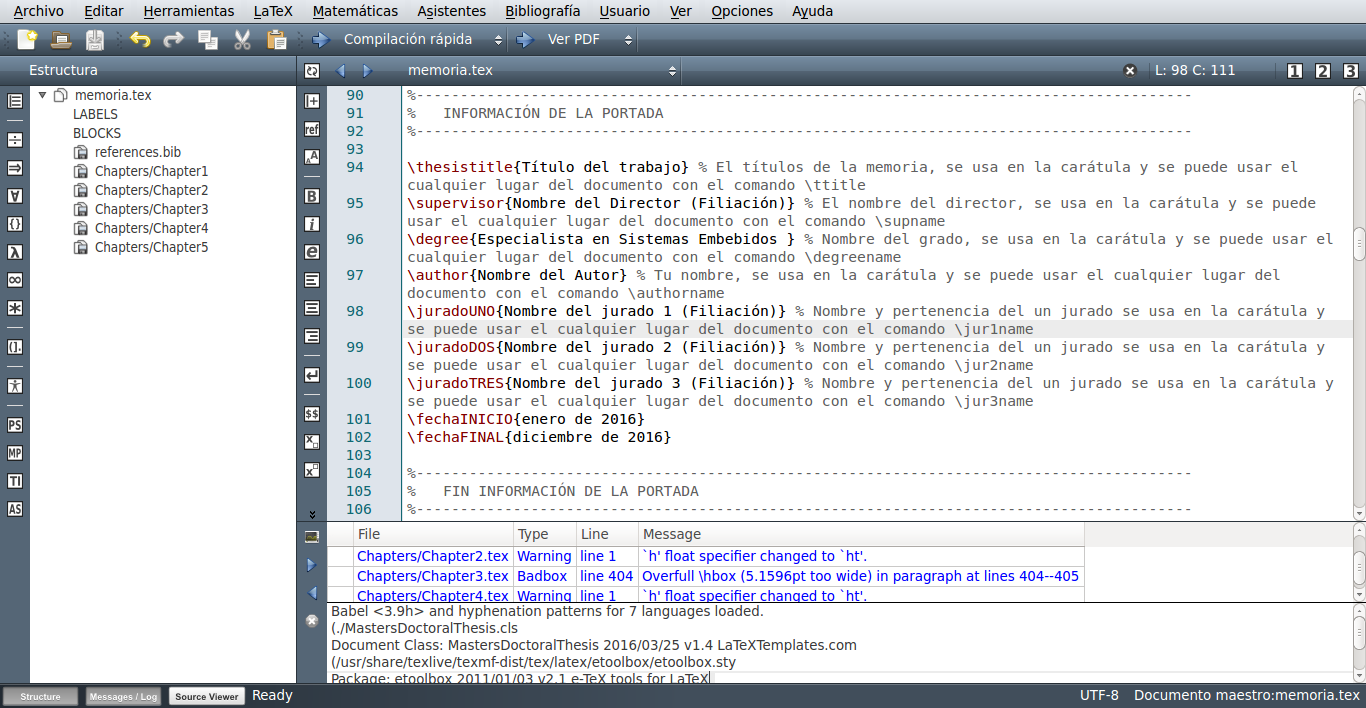
\includegraphics[width=.5\textwidth]{./Figures/texmaker.png}
% 	\caption{Entorno de trabajo de texMaker.}
% 	\label{fig:texmaker}
% \end{figure}

% \vspace{1cm}

% Notar que existe una vista llamada Estructura a la izquierda de la interfaz que nos permite abrir desde dentro del programa los archivos individuales de los capítulos.  A la derecha se encuentra una vista con el archivo propiamente dicho para su edición. Hacia la parte inferior se encuentra una vista del log con información de los resultados de la compilación.  En esta última vista pueden aparecen advertencias o \textit{warning}, que normalmente pueden ser ignorados, y los errores que se indican en color rojo y deben resolverse para que se genere el PDF de salida.

% Recordar que el archivo que se debe compilar con PDFLaTeX es \file{memoria.tex}, si se tratara de compilar alguno de los capítulos saldría un error.  Para salvar la molestia de tener que cambiar de archivo para compilar cada vez que se realice una modificación en un capítulo, se puede definir el archivo \file{memoria.tex} como ``documento maestro'' yendo al menú opciones -> ``definir documento actual como documento maestro'', lo que permite compilar con PDFLaTeX memoria.tex directamente desde cualquier archivo que se esté modificando . Se muestra esta opción en la figura \ref{fig:docMaestro}.

% \begin{figure}[h]
% 	\centering
% 	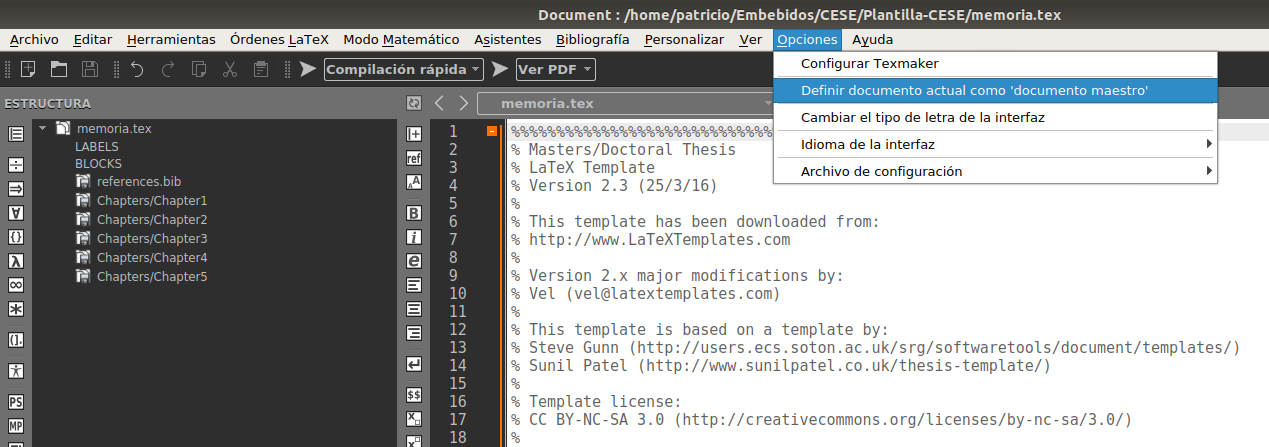
\includegraphics[width=\textwidth]{./Figures/docMaestro.png}
% 	\caption{Definir memoria.tex como documento maestro.}
% 	\label{fig:docMaestro}
% \end{figure}

% En el menú herramientas se encuentran las opciones de compilación.  Para producir un archivo PDF a partir de un archivo .tex se debe ejecutar PDFLaTeX (el shortcut es F6). Para incorporar nueva bibliografía se debe utilizar la opción BibTeX del mismo menú herramientas (el shortcut es F11).

% Notar que para actualizar las tablas de contenidos se debe ejecutar PDFLaTeX dos veces.  Esto se debe a que es necesario actualizar algunos archivos auxiliares antes de obtener el resultado final.  En forma similar, para actualizar las referencias bibliográficas se debe ejecutar primero PDFLaTeX, después BibTeX y finalmente PDFLaTeX dos veces por idénticos motivos.

% \section{Personalizando la plantilla, el archivo \file{memoria.tex}}
% \label{sec:FillingFile}

% Para personalizar la plantilla se debe incorporar la información propia en los distintos archivos \file{.tex}. 

% Primero abrir \file{memoria.tex} con TexMaker (o el editor de su preferencia). Se debe ubicar dentro del archivo el bloque de código titulado \emph{INFORMACIÓN DE LA PORTADA} donde se deben incorporar los primeros datos personales con los que se construirá automáticamente la portada.


% %----------------------------------------------------------------------------------------

% \section{El código del archivo \file{memoria.tex} explicado}

% El archivo \file{memoria.tex} contiene la estructura del documento y es el archivo de mayor jerarquía de la memoria.  Podría ser equiparable a la función \emph{main()} de un programa en C, o mejor dicho al archivo fuente .c donde se encuentra definida la función main().

% La estructura básica de cualquier documento de \LaTeX{} comienza con la definición de clase del documento, es seguida por un preámbulo donde se pueden agregar funcionalidades con el uso de \texttt{paquetes} (equiparables a bibliotecas de C), y finalmente, termina con el cuerpo del documento, donde irá el contenido de la memoria.

% \lstset{%
%   basicstyle=\small\ttfamily,
%   language=[LaTeX]{TeX}
% }

% \begin{lstlisting}
% \documentclass{article}  <- Definicion de clase
% \usepackage{listings}	 <- Preambulo

% \begin{document}	 <- Comienzo del contenido propio 
% 	Hello world!
% \end{document}
% \end{lstlisting}


% El archivo \file{memoria.tex} se encuentra densamente comentado para explicar qué páginas, secciones y elementos de formato está creando el código \LaTeX{} en cada línea. El código está dividido en bloques con nombres en mayúsculas para que resulte evidente qué es lo que hace esa porción de código en particular. Inicialmente puede parecer que hay mucho código \LaTeX{}, pero es principalmente código para dar formato a la memoria por lo que no requiere intervención del usuario de la plantilla.  Sí se deben personalizar con su información los bloques indicados como:

% \begin{itemize}
% 	\item Informacion de la memoria
% 	\item Resumen
% 	\item Agradecimientos
% 	\item Dedicatoria
% \end{itemize}

% El índice de contenidos, las listas de figura de tablas se generan en forma automática y no requieren intervención ni edición manual por parte del usuario de la plantilla. 

% En la parte final del documento se encuentran los capítulos y los apéndices.  Por defecto se incluyen los 5 capítulos propuestos que se encuentran en la carpeta /Chapters. Cada capítulo se debe escribir en un archivo .tex separado y se debe poner en la carpeta \emph{Chapters} con el nombre \file{Chapter1}, \file{Chapter2}, etc\ldots El código para incluir capítulos desde archivos externos se muestra a continuación.

% \begin{verbatim}
% 	% Chapter 1

\chapter{Introducción general} % Main chapter title

\label{Chapter1} % For referencing the chapter elsewhere, use \ref{Chapter1} 
\label{IntroGeneral}

Este capítulo tiene como propósito contextualizar el trabajo dentro del ámbito del consumo masivo y, en particular, de los modelos de negocio entre empresas (\textit{B2B}). Se expone la relevancia que adquiere la personalización comercial en este sector y los desafíos que surgen al gestionar un portafolio amplio de productos frente a una base heterogénea de clientes. A partir de esta perspectiva se describe el problema central que motiva el desarrollo de un motor de afinidad y se señalan las limitaciones de los enfoques tradicionales de recomendación en entornos de alta variabilidad y escasez de datos.

Asimismo, se realiza una revisión introductoria de los principales sistemas de
recomendación y de sus alcances en diferentes contextos, donde se destacan las
particularidades que distinguen al escenario de negocio entre empresas. Finalmente, se presentan la motivación, la relevancia y los objetivos del trabajo, con el fin de ofrecer al lector una visión clara del problema abordado, de la importancia de su resolución y del recorrido que seguirá la memoria en los capítulos posteriores.

%----------------------------------------------------------------------------------------

% Define some commands to keep the formatting separated from the content 
\newcommand{\keyword}[1]{\textbf{#1}}
\newcommand{\tabhead}[1]{\textbf{#1}}
\newcommand{\code}[1]{\texttt{#1}}
\newcommand{\file}[1]{\texttt{\bfseries#1}}
\newcommand{\option}[1]{\texttt{\itshape#1}}
\newcommand{\grados}{$^{\circ}$}

%----------------------------------------------------------------------------------------

\section{Marco de la propuesta}

La industria del consumo masivo constituye uno de los motores más importantes de la economía, caracterizada por un volumen elevado de transacciones, la alta frecuencia de compra y la amplia variedad de productos que la conforman. La magnitud de este sector, junto con la fuerte competencia existente, obliga a las compañías a buscar permanentemente mecanismos que les permitan diferenciarse y mejorar la relación con sus clientes.

En este entorno, la relación comercial se establece entre una empresa proveedora y una red extensa de clientes minoristas que funcionan como canales de llegada al consumidor final. Estos clientes presentan una gran diversidad en cuanto a tamaño, ubicación geográfica, recursos disponibles y patrones de demanda. La heterogeneidad de la red de distribución genera que cada establecimiento tenga necesidades distintas y reaccione de manera diferente frente a la oferta de productos. Bajo estas condiciones, una estrategia comercial homogénea resulta insuficiente, ya que no logra capturar las particularidades de cada cliente ni ofrecerle productos que se ajusten de manera adecuada a su realidad.

La necesidad de personalización surge entonces como un factor estratégico central. Adaptar la oferta a las características específicas de cada cliente no solo incrementa la probabilidad de aceptación de los productos sugeridos, sino que también permite optimizar el uso del canal comercial, fortalecer la relación de largo plazo y generar un impacto positivo en la eficiencia general del negocio. Las sugerencias ajustadas al contexto trascienden la idea de recomendar lo más vendido en términos absolutos: implica comprender la dinámica particular de cada cliente y priorizar aquellos productos que, dentro de un portafolio amplio, resulten más relevantes para su operación cotidiana.

A esta diversidad se suman factores que aumentan la complejidad del sector. La estacionalidad en la demanda, la influencia de promociones y campañas comerciales, la variabilidad en las preferencias de los consumidores finales y la constante rotación de productos dentro del catálogo configuran un escenario cambiante y difícil de predecir. La incorporación de artículos nuevos en el portafolio plantea, además, el desafío de la falta de contexto e información histórica que da perspectiva para guiar las recomendaciones.

En este marco, contar con herramientas que permitan personalizar la relación con cada cliente resulta indispensable. Un sistema capaz de priorizar los productos más relevantes para cada establecimiento aporta ventajas significativas: mejora la precisión de las recomendaciones, amplía la visibilidad de productos estratégicos, optimiza la gestión de los recursos comerciales y contribuye a consolidar vínculos más sólidos con los clientes minoristas. De esta manera, las recomendaciones a medida se convierten en un pilar fundamental para la sostenibilidad y la competitividad en el sector del consumo masivo.

%----------------------------------------------------------------------------------------

\section{Definición del problema}

La empresa en la que se desarrolla este trabajo pertenece al sector del consumo masivo y opera bajo un modelo de venta directa a una red amplia y heterogénea de clientes minoristas. Esta red está compuesta por autoservicios, kioscos y comercios tradicionales distribuidos en todo el territorio nacional, lo que permite alcanzar una cobertura superior a los trescientos mil puntos de venta. La magnitud de esta operación, sumada a la diversidad de formatos y capacidades de los clientes, convierte a la personalización en una necesidad estratégica. A ello se suma la complejidad de un portafolio que incluye un gran número de marcas y presentaciones, lo que multiplica las posibles combinaciones cliente–producto y genera un desafío de gestión a gran escala.

El reto principal radica en estimar con precisión el interés que cada cliente podría tener en cada producto dentro del portafolio. Hoy en día, las decisiones comerciales se apoyan principalmente en el historial de ventas o en la popularidad general de los artículos, lo que conduce a una oferta relativamente homogénea. Este enfoque ignora las particularidades de los clientes y no captura la relevancia contextual de los productos. El problema central se expresa, entonces, en la ausencia de mecanismos que permitan calcular un nivel de afinidad entre cliente y producto capaz de reflejar con realismo el grado de interés que un artículo puede despertar en un punto de venta específico en un momento determinado.

Este desafío se ve amplificado por una serie de batallas que la empresa enfrenta de manera cotidiana en su estrategia comercial. La primera de ellas es la necesidad de pasar de un enfoque reactivo, basado en compras históricas, hacia una estrategia proactiva que permita anticipar tendencias de consumo y orientar la oferta en consecuencia. Para ello es indispensable contar con una herramienta que adapte las recomendaciones de manera dinámica y alineada con el comportamiento observado en cada cliente.

Otra dimensión crítica es la optimización de recursos. La magnitud de la red comercial hace imposible abordar a todos los clientes con la misma intensidad, por lo que resulta fundamental identificar en qué productos y clientes concentrar los esfuerzos. Un motor de afinidad que jerarquice oportunidades de mayor impacto ofrece al equipo comercial la posibilidad de planificar visitas y diseñar ofertas más focalizadas, lo que mejora la eficiencia del canal.

La constante rotación del portafolio también representa un desafío de gran magnitud. Una proporción significativa de los productos se renueva cada año, lo que obliga a dar visibilidad a artículos sin historial de ventas y, al mismo tiempo, sostener el desempeño de categorías tradicionales. Este problema de arranque en frío limita la capacidad de los enfoques tradicionales para recomendar productos nuevos o poco frecuentes, lo que retrasa su incorporación en los puntos de venta y afecta el posicionamiento de la innovación en el mercado.

De manera similar, la inserción de nuevos clientes en la red sin historial de compras constituye un reto adicional. Cada semana se incorporan comercios que aún no cuentan con registros transaccionales suficientes para perfilar sus preferencias. Estos clientes suelen recibir sugerencias genéricas o basadas en promedios de segmentos, lo que reduce el atractivo de la oferta inicial y dificulta su integración temprana al canal digital. Una solución efectiva debería ser capaz de recomendar productos relevantes aun en ausencia de historial, al aprovechar señales contextuales y patrones de clientes similares.

La estacionalidad y las promociones constituyen otro factor de complejidad. La demanda de determinados productos fluctúa de manera pronunciada según la época del año o las campañas comerciales en curso. Un producto que en un período presenta alta relevancia puede perder vigencia en el siguiente, lo que provoca que reglas estáticas de recomendación queden rápidamente obsoletas. Para sostener la efectividad en este entorno dinámico se requiere un sistema flexible y capaz de adaptarse a variaciones temporales.

En conjunto, estos factores configuran un escenario donde la falta de personalización impacta de manera directa en los resultados del negocio. Sin un mecanismo que integre de manera sistemática los datos disponibles, se generan listas de productos poco relevantes para los clientes, se desperdician oportunidades de venta cruzada y se dificulta la adopción de innovaciones. Asimismo, el equipo comercial se ve limitado por información fragmentada, lo que reduce su capacidad de diseñar acciones específicas y de extraer valor de la gran cantidad de datos generados en el canal digital.

La solución propuesta apunta a superar estas limitaciones mediante el desarrollo de un motor de afinidad que calcule de forma periódica la relevancia de cada producto para cada cliente, y que integra señales transaccionales, interacciones digitales y atributos contextuales. Este motor tiene como objetivo generar rankings personalizados que orienten las recomendaciones tanto en el canal digital como en la gestión directa del equipo comercial. De esta forma, se busca avanzar hacia una estrategia más precisa, escalable y alineada con los objetivos de negocio, lo que habilita una gestión proactiva de portafolio y mejora la relación con los clientes de la red.

%----------------------------------------------------------------------------------------

\section{Estado del arte}

El estado del arte permite ubicar este trabajo dentro de la evolución de los sistemas de recomendación. En esta sección se revisan los principales \textit{benchmarks} en entornos B2C, los aportes de la literatura en contextos B2B y un caso de implementación en Brasil, para finalmente sintetizar los aprendizajes y señalar la brecha que orienta esta propuesta.

\subsection{Referencias en sistemas de recomendación}

El campo de los sistemas de recomendación se consolidó en los últimos veinte años como una de las áreas más dinámicas dentro de la inteligencia artificial aplicada. Sus desarrollos se originaron en entornos de consumo directo al público, donde el volumen de usuarios y la abundancia de señales digitales permitieron mejorar rápidamente la precisión y escalabilidad. A lo largo de este proceso, distintos hitos se transformaron en referencias obligadas y definieron \textit{benchmarks} de la disciplina.

Uno de los puntos de inflexión fue el concurso Netflix Prize \cite{ARTICLE:NetflixPrize}, que impulsó avances en factorización matricial y consolidó métricas de ranking como \textit{recall} y \textit{precision} en el análisis de desempeño. En paralelo, Amazon desarrolló un motor de recomendaciones basado en filtrado colaborativo \textit{item-to-item}, reconocido por su capacidad de escalar en catálogos extensos y mantener robustez frente a grandes volúmenes de transacciones. MovieLens \cite{ARTICLE:MovieLens} se transformó en el dataset académico más utilizado, al servir como estándar para comparar algoritmos y validar resultados de manera consistente. Finalmente, plataformas como Spotify y YouTube llevaron la disciplina hacia modelos secuenciales y de aprendizaje profundo, capaces de personalizar en tiempo real a partir de interacciones en sesiones cortas.

Estos casos muestran cómo los sistemas de recomendación se convirtieron en el núcleo de la personalización digital y establecieron estándares en cuanto a precisión, escalabilidad y diversidad. Al mismo tiempo, reflejan un sesgo hacia contextos de  \textit{Business to Customer (B2C)}, donde las interacciones con consumidores finales son abundantes, explícitas y fácilmente trazables.

\subsection{Sistemas de recomendación en B2B}

En entornos de negocio entre empresas, la adopción de sistemas de recomendación es mucho más incipiente. La literatura identifica que, a diferencia de lo que ocurre en B2C, los procesos de compra en B2B suelen involucrar múltiples actores, ciclos de decisión más largos y una relación de largo plazo entre proveedor y cliente. Estas particularidades hacen que las soluciones desarrolladas para consumo final no se trasladen de forma directa.

El estudio presentado en \cite{ARTICLE:1} resalta el potencial de estas herramientas en B2B, al destacar que pueden reducir los costos de búsqueda, fortalecer vínculos comerciales y facilitar la introducción de productos en portafolios complejos. Sin embargo, también identifica desafíos clave: la necesidad de integrar datos dispersos de distintas fuentes, la importancia de la interpretabilidad para ganar confianza en decisiones de compra de alto valor y la dificultad de escalar modelos en contextos de menor densidad transaccional.

En síntesis, si bien existe un reconocimiento académico del valor que los sistemas de recomendación pueden aportar en B2B, las implementaciones concretas son todavía escasas y carecen de estandarización. Esto genera una brecha significativa entre el potencial identificado y la práctica real, que representa una oportunidad de innovación para sectores como el consumo masivo.

\subsection{Caso de implementación}

Un antecedente particularmente relevante proviene de la propia organización, a través de la implementación de un sistema de recomendación en Brasil dentro de la plataforma digital BEES \cite{REPORT:1}. Este desarrollo tuvo como objetivo priorizar productos para cada punto de venta a gran escala, con el fin de reemplazar procesos manuales que en el pasado se realizaban en planillas y que resultaban poco eficientes.

El algoritmo principal implementado fue un filtrado colaborativo para feedback implícito, concretado mediante factorización matricial con el método \textit{Alternating Least Squares (ALS)}. El modelo utilizó como insumos tanto el historial de compras como señales digitales generadas en la aplicación, e incluyó búsquedas, visualizaciones de productos e interacciones con el carrito de compras. De este modo, se logró reducir sustancialmente la cantidad de recomendaciones enfocándolas en productos con mayor interés para el cliente, lo que marcó un avance significativo en la capacidad de personalizar la oferta a cada punto de venta.

Los resultados demostraron la viabilidad de este tipo de soluciones en un entorno B2B real y de gran escala. Sin embargo, también dejaron en evidencia limitaciones relevantes. La dependencia casi exclusiva del historial transaccional reforzó el problema del arranque en frío, tanto para productos recién incorporados como para clientes nuevos sin registros suficientes. Además, el sistema presentó limitaciones en diversidad de recomendaciones, ya que tendía a reforzar productos populares, y careció de un componente explícito para alinear los resultados con prioridades estratégicas de negocio.

El mismo documento identifica líneas de mejora hacia el futuro, como la incorporación de modelos híbridos que integren atributos de clientes y productos, el desarrollo de algoritmos de \textit{clustering} para agrupar unidades de negocio con características similares y la inclusión de mecanismos que permitan diversificar resultados. Estas observaciones resultan especialmente valiosas para orientar el diseño de una solución adaptada al contexto argentino.

\subsection{Lecciones aprendidas}

El recorrido presentado permite extraer tres conclusiones principales. En primer lugar, los benchmarks internacionales muestran que los sistemas de recomendación son capaces de transformar industrias enteras cuando logran combinar precisión, escalabilidad y diversidad. En segundo lugar, la literatura sobre B2B reconoce la oportunidad de trasladar estos beneficios, pero también evidencia la falta de soluciones maduras que contemplen las particularidades de este tipo de relaciones comerciales. Finalmente, el caso de Brasil demuestra que es posible implementar un motor de recomendaciones en un contexto de consumo masivo B2B, pero también que persisten limitaciones en arranque en frío, diversidad y alineación con objetivos de negocio.

A modo de síntesis, la tabla \ref{tab:estado_arte} resume las ventajas y desventajas de cada uno de los enfoques revisados, e incluye la brecha identificada en el contexto argentino que motiva el desarrollo de un motor de afinidad adaptado a la realidad local. Este resumen permite enfatizar la necesidad de avanzar hacia un sistema que integre señales transaccionales y digitales, incorpore criterios estratégicos de negocio y se apoye en técnicas modernas de aprendizaje automático y profundo. El objetivo es superar las restricciones de los enfoques tradicionales y aportar un valor diferencial en la gestión comercial de la empresa en Argentina.

\begin{table}[H]
\centering
\caption[Ventajas y desventajas de enfoques en recomendación]{Ventajas y desventajas de los enfoques revisados.}
\label{tab:estado_arte}
\begin{tabularx}{\textwidth}{>{\hsize=0.5\hsize}X >{\hsize=1.25\hsize}X >{\hsize=1.25\hsize}X}
\toprule
Enfoque / Caso & Ventajas principales & Desventajas principales \\
\midrule
Benchmarks \emph{B2C} (Netflix, Amazon, etc.) &
Alta precisión y escalabilidad. Abundancia de datos y señales digitales. Estándares de evaluación consolidados. &
Contextos con abundancia de \emph{feedback} explícito/implícito, poco comparables al \emph{B2B}. No consideran objetivos de negocio específicos. \\
\midrule
Literatura \emph{B2B} &
Reconoce particularidades de clientes empresariales. Identifica beneficios en reducción de costos y fortalecimiento de relaciones. &
Pocas implementaciones reales. Escasa estandarización de métricas y \emph{datasets}. Desafíos de interpretabilidad y escalabilidad. \\
\midrule
Caso Brasil (BEES) &
Demostró viabilidad en gran escala. Integró compras e interacciones digitales. Mejora clara frente a procesos manuales. &
Dependencia fuerte del historial transaccional (arranque en frío). Limitaciones en diversidad y alineación con objetivos estratégicos. \\
\midrule
Brecha en Argentina &
Oportunidad de adaptar aprendizajes globales y regionales. Potencial de integrar señales contextuales y digitales. Aplicación de técnicas modernas de aprendizaje automático y profundo. &
Falta de solución probada en el contexto local. Mayor heterogeneidad y escala que en otros países. \\
\bottomrule
\end{tabularx}
\end{table}

%----------------------------------------------------------------------------------------

\section{Motivación}

La definición del problema mostró que la empresa enfrenta limitaciones para identificar con precisión qué productos resultan más relevantes para cada cliente en cada momento, debido a factores como la rotación del portafolio, la estacionalidad de la demanda y la incorporación de nuevos clientes sin historial. El estado del arte, por su parte, evidencia que si bien existen avances notables en sistemas de recomendación y casos aplicados en entornos B2C, aún persiste una brecha en cuanto a soluciones robustas y adaptadas a escenarios B2B de consumo masivo.

La motivación de este trabajo surge de esa intersección: un problema claramente identificado en la operación local y un campo de conocimiento que ofrece enfoques valiosos pero todavía insuficientes para resolverlo en toda su complejidad. El diferencial de esta propuesta reside en integrar múltiples fuentes de información, transaccionales, digitales y contextuales, dentro de un motor de afinidad diseñado específicamente para el mercado argentino. Además, el trabajo incorpora la orientación explícita a objetivos de negocio y el uso de prácticas modernas de aprendizaje automático, aprendizaje profundo y MLOps, con el fin de garantizar escalabilidad, trazabilidad y alineación estratégica.

En este sentido, el trabajo no busca reproducir soluciones existentes, sino avanzar hacia un sistema que combine la rigurosidad técnica con la aplicabilidad práctica en un contexto desafiante, y que aporte un valor diferencial tanto en la gestión comercial de la empresa como en la evolución del conocimiento sobre sistemas de recomendación en consumo masivo B2B.


%----------------------------------------------------------------------------------------

\section{Objetivos y alcance}

El propósito general de este trabajo es desarrollar un motor de afinidad que permita generar recomendaciones personalizadas de productos para cada cliente de la red de la empresa. El sistema se plantea como una herramienta capaz de integrar información transaccional, señales digitales y atributos contextuales con el fin de optimizar la gestión comercial, mejorar la efectividad de las sugerencias y facilitar la adopción de categorías estratégicas.

A partir de este objetivo general se desprenden metas específicas que orientan el desarrollo. En primer lugar, se busca analizar en detalle las fuentes de datos disponibles y transformarlas en insumos útiles para el modelado. Sobre esta base, se plantea la construcción de variables que reflejen el comportamiento de compra, las características de los productos y el contexto de cada cliente. Un segundo objetivo es implementar y comparar distintos enfoques de modelado, desde métodos de referencia hasta técnicas de factorización, modelos híbridos y arquitecturas profundas, con el objetivo de evaluar su desempeño con métricas de ranking como \textit{recall@K, MAP@K}, cobertura y diversidad. De manera complementaria, se incluye la necesidad de diseñar estrategias que permitan afrontar el arranque en frío, tanto de productos recién incorporados al portafolio como de clientes nuevos sin historial de compras. Finalmente, se busca establecer un pipeline de entrenamiento y despliegue con prácticas de MLOps que garantice trazabilidad, reproducibilidad y escalabilidad del sistema.

El alcance del trabajo se limita a la construcción y evaluación de un prototipo funcional en un entorno controlado con datos reales de la empresa. Esto implica el análisis y preparación de la información, el desarrollo de modelos de recomendación y la evaluación de su desempeño a través de métricas definidas, e incluye escenarios de robustez frente a la incorporación de productos y clientes nuevos. También, se contempla el diseño conceptual de la integración del motor con el canal digital y el apoyo al trabajo del equipo comercial.


%----------------------------------------------------------------------------------------
% \section{Aprendiendo \LaTeX{}}

% \LaTeX{} no es \textsc{WYSIWYG} (What You See is What You Get), a diferencia de los procesadores de texto como Microsoft Word o Pages de Apple o incluso LibreOffice en el mundo open-source. En lugar de ello, un documento escrito para \LaTeX{} es en realidad un archivo de texto simple o llano que \emph{no contiene formato} . Nosotros le decimos a \LaTeX{} cómo deseamos que se aplique el formato en el documento final escribiendo comandos simples entre el texto, por ejemplo, si quiero usar texto en itálicas para dar énfasis, escribo \verb|\it{texto}| y pongo el texto que quiero en itálicas entre medio de las llaves. Esto significa que \LaTeX{} es un lenguaje del tipo \enquote{mark-up}, muy parecido a HTML.

% \subsection{Una introducción (no tan corta) a \LaTeX{}}

% Si sos nuevo en \LaTeX{}, hay un muy buen libro electrónico - disponible gratuitamente en Internet como un archivo PDF - llamado, \enquote{A (not so short) Introduction to \LaTeX{}}. El título del libro es generalmente acortado a simplemente \emph{lshort}. Puede descargar la versión más reciente en inglés (ya que se actualiza de vez en cuando) desde aquí:
% \url{http://www.ctan.org/tex-archive/info/lshort/english/lshort.pdf}

% Se puede encontrar la versión en español en la lista en esta página: \url{http://www.ctan.org/tex-archive/info/lshort/}

% \subsubsection{Una subsubsección}

% Acá tiene un ejemplo de una ``subsubsección'' que es el cuarto nivel de ordenamiento del texto, después de capítulo, sección y subsección.  Como se puede ver, las subsubsecciones no van numeradas en el cuerpo del documento ni en el índice.  El formato está definido por la plantilla y no debe ser modificado.

% \subsection{Guía matemática rápida para \LaTeX{}}

% Si estás escribiendo un documento con mucho contenido matemático, entonces es posible que desees leer el documento de la AMS (American Mathematical Society) llamado, \enquote{A Short Math Guide for \LaTeX{}}. Se puede encontrar en línea en el siguiente link: \url{http://www.ams.org/tex/amslatex.html} en la sección \enquote{Additional Documentation} hacia la parte inferior de la página.


% %----------------------------------------------------------------------------------------

% \section{Utilizando esta plantilla}

% Si estás familiarizado con \LaTeX{}, entonces podés explorar la estructura de directorios de esta plantilla y proceder a personalizarla agregando tu información en el bloque \emph{INFORMACIÓN DE LA PORTADA} en el archivo \file{memoria.tex}.  

% Se puede continuar luego modificando el resto de los archivos siguiendo los lineamientos que se describen en la sección \ref{sec:FillingFile} en la página \pageref{sec:FillingFile}.

% Debés asegurarte de leer el capítulo \ref{Chapter2} acerca de las convenciones utilizadas para las Memoria de los Trabajos Finales de la \degreename.

% Si sos nuevo en \LaTeX{}, se recomienda que continúes leyendo el documento ya que contiene información básica para aprovechar el potencial de esta herramienta.


% %----------------------------------------------------------------------------------------

% \section{Qué incluye esta plantilla}

% \subsection{Carpetas}

% Esta plantilla se distribuye como una único archivo .zip que se puede descomprimir en varios archivos y carpetas. Asimismo, se puede consultar el repositorio git para obtener la última versión de los archivos, \url{https://github.com/patriciobos/Plantilla-CESE.git}. Los nombres de las carpetas son, o pretender ser, auto-explicativos.

% \keyword{Appendices} -- Esta es la carpeta donde se deben poner los apéndices. Cada apéndice debe ir en su propio archivo \file{.tex}. Se incluye un ejemplo y una plantilla en la carpeta.

% \keyword{Chapters} -- Esta es la carpeta donde se deben poner los capítulos de la memoria. Cada capítulo debe ir un su propio archivo \file{.tex} por separado.  Se ofrece por defecto, la siguiente estructura de capítulos y se recomienda su utilización dentro de lo posible:

% \begin{itemize}
% \item Capítulo 1: Introducción general	
% \item Capítulo 2: Introducción específica
% \item Capítulo 3: Diseño e implementación
% \item Capítulo 4: Ensayos y resultados
% \item Capítulo 5: Conclusiones

% \end{itemize}

% Esta estructura de capítulos es la que se recomienda para las memorias de la especialización.

% \keyword{Figures} -- Esta carpeta contiene todas las figuras de la memoria.  Estas son las versiones finales de las imágenes que van a ser incluidas en la memoria.  Pueden ser imágenes en formato \textit{raster}\footnote{\url{https://en.wikipedia.org/wiki/Raster_graphics}} como \file{.png}, \file{.jpg} o en formato vectoriales\footnote{\url{https://en.wikipedia.org/wiki/Vector_graphics}} como \file{.pdf}, \file{.ps}.  Se debe notar que utilizar imágenes vectoriales disminuye notablemente el peso del documento final y acelera el tiempo de compilación por lo que es recomendable su utilización siempre que sea posible.

% \subsection{Archivos}

% También están incluidos varios archivos, la mayoría de ellos son de texto plano y se puede ver su contenido en un editor de texto. Después de la compilación inicial, se verá que más archivos auxiliares son creados por \ LaTeX{} o BibTeX, pero son de uso interno y no es necesario hacer nada en particular con ellos.  Toda la información necesaria para compilar el documento se encuentra en los archivos \file{.tex}, \file{.bib}, \file{.cls} y en las imágenes de la carpeta Figures.

% \keyword{referencias.bib} - este es un archivo importante que contiene toda la información de referencias bibliográficas que se utilizarán para las citas en la memoria en conjunto con BibTeX. Usted puede escribir las entradas bibliográficas en forma manual, aunque existen también programas de gestión de referencias que facilitan la creación y gestión de las referencias y permiten exportarlas en formato BibTeX.  También hay disponibles sitios web como \url{books.google.com} que permiten obtener toda la información necesaria para una cita en formato BibTeX. Ver sección \ref{sec:biblio}

% \keyword{MastersDoctoralThesis.cls} -- este es un archivo importante. Es el archivos con la clase que le informa a \LaTeX{} cómo debe dar formato a la memoria. El usuario de la plantilla no debería necesitar modificar nada de este archivo.

% \keyword{memoria.pdf} -- esta es su memoria con una tipografía bellamente compuesta (en formato de archivo PDF) creado por \LaTeX{}. Se distribuye con la plantilla y después de compilar por primera vez sin hacer ningún cambio se debería obtener una versión idéntica a este documento.

% \keyword{memoria.tex} -- este es un archivo importante. Este es el archivo que tiene que compilar \LaTeX{} para producir la memoria como un archivo PDF. Contiene un marco de trabajo y estructuras que le indican a \LaTeX{} cómo diagramar la memoria.  Está altamente comentado para que se pueda entender qué es lo que realiza cada línea de código y por qué está incluida en ese lugar.  En este archivo se debe completar la información personalizada de las primeras sección según se indica en la sección \ref{sec:FillingFile}.

% Archivos que \emph{no} forman parte de la distribución de la plantilla pero que son generados por \LaTeX{} como archivos auxiliares necesarios para la producción de la memoria.pdf son:

% \keyword{memoria.aux} -- este es un archivo auxiliar generado por \LaTeX{}, si se borra \LaTeX{} simplemente lo regenera cuando se compila el archivo principal \file{memoria.tex}.

% \keyword{memoria.bbl} -- este es un archivo auxiliar generado por BibTeX, si se borra BibTeX simplemente lo regenera cuando se compila el archivo principal \file{memoria.tex}. Mientras que el archivo \file{.bib} contiene todas las referencias que hay, este archivo \file{.bbl} contine sólo las referencias que han sido citadas y se utiliza para la construcción de la bibiografía.

% \keyword{memoria.blg} -- este es un archivo auxiliar generado por BibTeX, si se borra BibTeX simplemente lo regenera cuando se compila el archivo principal \file{memoria.tex}.

% \keyword{memoria.lof} -- este es un archivo auxiliar generado por \LaTeX{}, si se borra \LaTeX{} simplemente lo regenera cuando se compila el archivo principal \file{memoria.tex}.  Le indica a \LaTeX{} cómo construir la sección \emph{Lista de Figuras}.
 
% \keyword{memoria.log} --  este es un archivo auxiliar generado por \LaTeX{}, si se borra \LaTeX{} simplemente lo regenera cuando se compila el archivo principal \file{memoria.tex}. Contiene mensajes de \LaTeX{}. Si se reciben errores o advertencias durante la compilación, se guardan en este archivo \file{.log}.

% \keyword{memoria.lot} -- este es un archivo auxiliar generado por \LaTeX{}, si se borra \LaTeX{} simplemente lo regenera cuando se compila el archivo principal \file{memoria.tex}.  Le indica a \LaTeX{} cómo construir la sección \emph{Lista de Tablas}.

% \keyword{memoria.out} -- este es un archivo auxiliar generado por \LaTeX{}, si se borra \LaTeX{} simplemente lo regenera cuando se compila el archivo principal \file{memoria.tex}.

% De esta larga lista de archivos, sólo aquellos con la extensión \file{.bib}, \file{.cls} y \file{.tex} son importantes.  Los otros archivos auxiliares pueden ser ignorados o borrados ya que \LaTeX{} y BibTeX los regenerarán durante la compilación.

% %----------------------------------------------------------------------------------------

% \section{Entorno de trabajo}

% Ante de comenzar a editar la plantilla debemos tener un editor \LaTeX{} instalado en nuestra computadora.  En forma análoga a lo que sucede en lenguaje C, que se puede crear y editar código con casi cualquier editor, existen ciertos entornos de trabajo que nos pueden simplificar mucho la tarea.  En este sentido, se recomienda, sobre todo para los principiantes en \LaTeX{} la utilización de TexMaker, un programa gratuito y multi-plantaforma que está disponible tanto para windows como para sistemas GNU/linux.

% La versión más reciente de TexMaker es la 4.5 y se puede descargar del siguiente link: \url{http://www.xm1math.net/texmaker/download.html}. Se puede consultar el manual de usuario en el siguiente link: \url{http://www.xm1math.net/texmaker/doc.html}.
 

% \subsection{Paquetes adicionales}

% Si bien durante el proceso de instalación de TexMaker, o cualquier otro editor que se haya elegido, se instalarán en el sistema los paquetes básicos necesarios para trabajar con \LaTeX{}, la plantilla de los trabajos de Especialización y Maestría requieren de paquete adicionales.

% Se indican a continuación los comandos que se deben introducir en la consola de Ubuntu (ctrl + alt + t) para instalarlos:

% \begin{lstlisting}[language=bash]
%   $ sudo apt install texlive-lang-spanish texlive-science 
%   $ sudo apt install texlive-bibtex-extra biber
%   $ sudo apt install texlive texlive-fonts-recommended
%   $ sudo apt install texlive-latex-extra
% \end{lstlisting}


% \subsection{Configurando TexMaker}
% \label{subsec:configurando}



% Una vez instalado el programa y los paquetes adicionales se debe abrir el archivo memoria.tex con el editor para ver una pantalla similar a la que se puede apreciar en la figura \ref{fig:texmaker}. 
% Una vez instalado el programa y los paquetes adicionales se debe abrir el archivo memoria.tex con el editor para ver una pantalla similar a la que se puede apreciar en la figura \ref{fig:texmaker}. 
% Una vez instalado el programa y los paquetes adicionales se debe abrir el archivo memoria.tex con el editor para ver una pantalla similar a la que se puede apreciar en la figura \ref{fig:texmaker}. 
% Una vez instalado el programa y los paquetes adicionales se debe abrir el archivo memoria.tex con el editor para ver una pantalla similar a la que se puede apreciar en la figura \ref{fig:texmaker}. 

% \vspace{1cm}

% \begin{figure}[htbp]
% 	\centering
% 	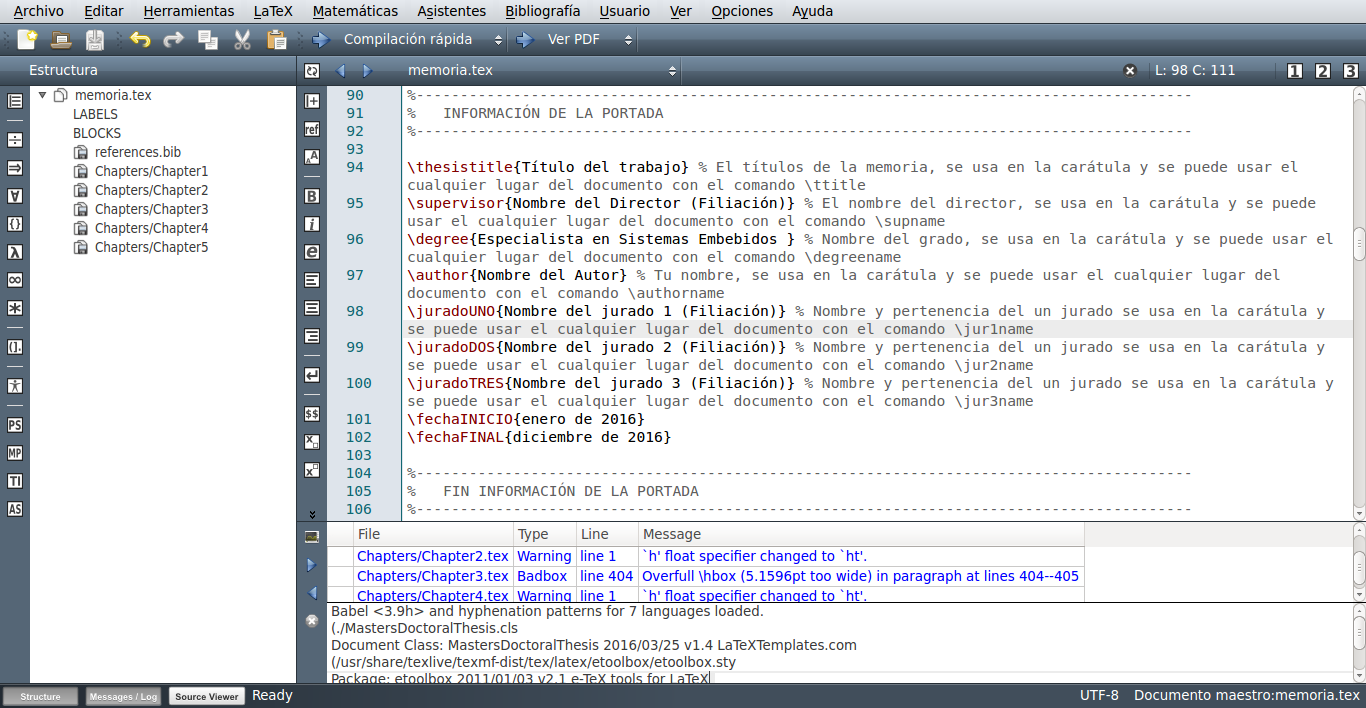
\includegraphics[width=.5\textwidth]{./Figures/texmaker.png}
% 	\caption{Entorno de trabajo de texMaker.}
% 	\label{fig:texmaker}
% \end{figure}

% \vspace{1cm}

% Notar que existe una vista llamada Estructura a la izquierda de la interfaz que nos permite abrir desde dentro del programa los archivos individuales de los capítulos.  A la derecha se encuentra una vista con el archivo propiamente dicho para su edición. Hacia la parte inferior se encuentra una vista del log con información de los resultados de la compilación.  En esta última vista pueden aparecen advertencias o \textit{warning}, que normalmente pueden ser ignorados, y los errores que se indican en color rojo y deben resolverse para que se genere el PDF de salida.

% Recordar que el archivo que se debe compilar con PDFLaTeX es \file{memoria.tex}, si se tratara de compilar alguno de los capítulos saldría un error.  Para salvar la molestia de tener que cambiar de archivo para compilar cada vez que se realice una modificación en un capítulo, se puede definir el archivo \file{memoria.tex} como ``documento maestro'' yendo al menú opciones -> ``definir documento actual como documento maestro'', lo que permite compilar con PDFLaTeX memoria.tex directamente desde cualquier archivo que se esté modificando . Se muestra esta opción en la figura \ref{fig:docMaestro}.

% \begin{figure}[h]
% 	\centering
% 	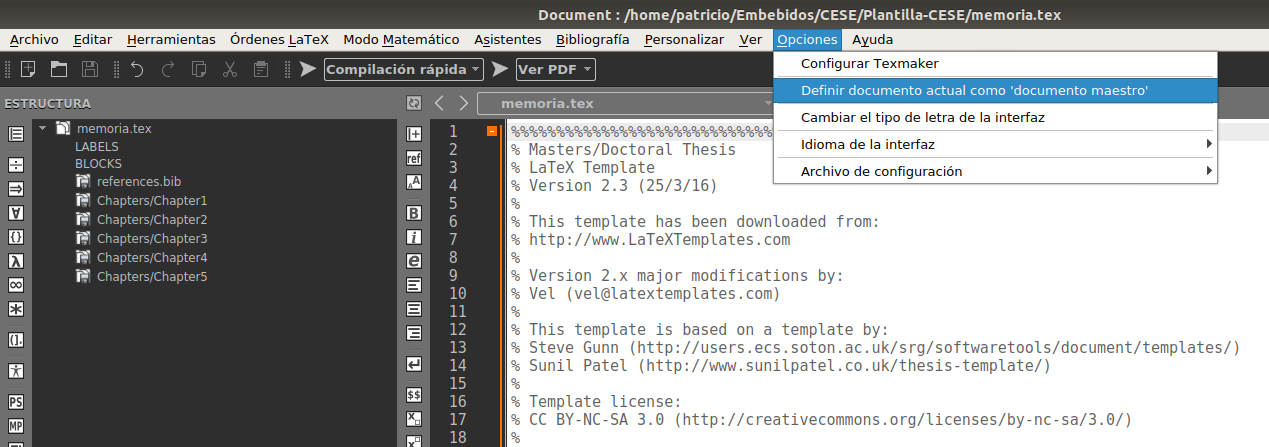
\includegraphics[width=\textwidth]{./Figures/docMaestro.png}
% 	\caption{Definir memoria.tex como documento maestro.}
% 	\label{fig:docMaestro}
% \end{figure}

% En el menú herramientas se encuentran las opciones de compilación.  Para producir un archivo PDF a partir de un archivo .tex se debe ejecutar PDFLaTeX (el shortcut es F6). Para incorporar nueva bibliografía se debe utilizar la opción BibTeX del mismo menú herramientas (el shortcut es F11).

% Notar que para actualizar las tablas de contenidos se debe ejecutar PDFLaTeX dos veces.  Esto se debe a que es necesario actualizar algunos archivos auxiliares antes de obtener el resultado final.  En forma similar, para actualizar las referencias bibliográficas se debe ejecutar primero PDFLaTeX, después BibTeX y finalmente PDFLaTeX dos veces por idénticos motivos.

% \section{Personalizando la plantilla, el archivo \file{memoria.tex}}
% \label{sec:FillingFile}

% Para personalizar la plantilla se debe incorporar la información propia en los distintos archivos \file{.tex}. 

% Primero abrir \file{memoria.tex} con TexMaker (o el editor de su preferencia). Se debe ubicar dentro del archivo el bloque de código titulado \emph{INFORMACIÓN DE LA PORTADA} donde se deben incorporar los primeros datos personales con los que se construirá automáticamente la portada.


% %----------------------------------------------------------------------------------------

% \section{El código del archivo \file{memoria.tex} explicado}

% El archivo \file{memoria.tex} contiene la estructura del documento y es el archivo de mayor jerarquía de la memoria.  Podría ser equiparable a la función \emph{main()} de un programa en C, o mejor dicho al archivo fuente .c donde se encuentra definida la función main().

% La estructura básica de cualquier documento de \LaTeX{} comienza con la definición de clase del documento, es seguida por un preámbulo donde se pueden agregar funcionalidades con el uso de \texttt{paquetes} (equiparables a bibliotecas de C), y finalmente, termina con el cuerpo del documento, donde irá el contenido de la memoria.

% \lstset{%
%   basicstyle=\small\ttfamily,
%   language=[LaTeX]{TeX}
% }

% \begin{lstlisting}
% \documentclass{article}  <- Definicion de clase
% \usepackage{listings}	 <- Preambulo

% \begin{document}	 <- Comienzo del contenido propio 
% 	Hello world!
% \end{document}
% \end{lstlisting}


% El archivo \file{memoria.tex} se encuentra densamente comentado para explicar qué páginas, secciones y elementos de formato está creando el código \LaTeX{} en cada línea. El código está dividido en bloques con nombres en mayúsculas para que resulte evidente qué es lo que hace esa porción de código en particular. Inicialmente puede parecer que hay mucho código \LaTeX{}, pero es principalmente código para dar formato a la memoria por lo que no requiere intervención del usuario de la plantilla.  Sí se deben personalizar con su información los bloques indicados como:

% \begin{itemize}
% 	\item Informacion de la memoria
% 	\item Resumen
% 	\item Agradecimientos
% 	\item Dedicatoria
% \end{itemize}

% El índice de contenidos, las listas de figura de tablas se generan en forma automática y no requieren intervención ni edición manual por parte del usuario de la plantilla. 

% En la parte final del documento se encuentran los capítulos y los apéndices.  Por defecto se incluyen los 5 capítulos propuestos que se encuentran en la carpeta /Chapters. Cada capítulo se debe escribir en un archivo .tex separado y se debe poner en la carpeta \emph{Chapters} con el nombre \file{Chapter1}, \file{Chapter2}, etc\ldots El código para incluir capítulos desde archivos externos se muestra a continuación.

% \begin{verbatim}
% 	% Chapter 1

\chapter{Introducción general} % Main chapter title

\label{Chapter1} % For referencing the chapter elsewhere, use \ref{Chapter1} 
\label{IntroGeneral}

Este capítulo tiene como propósito contextualizar el trabajo dentro del ámbito del consumo masivo y, en particular, de los modelos de negocio entre empresas (\textit{B2B}). Se expone la relevancia que adquiere la personalización comercial en este sector y los desafíos que surgen al gestionar un portafolio amplio de productos frente a una base heterogénea de clientes. A partir de esta perspectiva se describe el problema central que motiva el desarrollo de un motor de afinidad y se señalan las limitaciones de los enfoques tradicionales de recomendación en entornos de alta variabilidad y escasez de datos.

Asimismo, se realiza una revisión introductoria de los principales sistemas de
recomendación y de sus alcances en diferentes contextos, donde se destacan las
particularidades que distinguen al escenario de negocio entre empresas. Finalmente, se presentan la motivación, la relevancia y los objetivos del trabajo, con el fin de ofrecer al lector una visión clara del problema abordado, de la importancia de su resolución y del recorrido que seguirá la memoria en los capítulos posteriores.

%----------------------------------------------------------------------------------------

% Define some commands to keep the formatting separated from the content 
\newcommand{\keyword}[1]{\textbf{#1}}
\newcommand{\tabhead}[1]{\textbf{#1}}
\newcommand{\code}[1]{\texttt{#1}}
\newcommand{\file}[1]{\texttt{\bfseries#1}}
\newcommand{\option}[1]{\texttt{\itshape#1}}
\newcommand{\grados}{$^{\circ}$}

%----------------------------------------------------------------------------------------

\section{Marco de la propuesta}

La industria del consumo masivo constituye uno de los motores más importantes de la economía, caracterizada por un volumen elevado de transacciones, la alta frecuencia de compra y la amplia variedad de productos que la conforman. La magnitud de este sector, junto con la fuerte competencia existente, obliga a las compañías a buscar permanentemente mecanismos que les permitan diferenciarse y mejorar la relación con sus clientes.

En este entorno, la relación comercial se establece entre una empresa proveedora y una red extensa de clientes minoristas que funcionan como canales de llegada al consumidor final. Estos clientes presentan una gran diversidad en cuanto a tamaño, ubicación geográfica, recursos disponibles y patrones de demanda. La heterogeneidad de la red de distribución genera que cada establecimiento tenga necesidades distintas y reaccione de manera diferente frente a la oferta de productos. Bajo estas condiciones, una estrategia comercial homogénea resulta insuficiente, ya que no logra capturar las particularidades de cada cliente ni ofrecerle productos que se ajusten de manera adecuada a su realidad.

La necesidad de personalización surge entonces como un factor estratégico central. Adaptar la oferta a las características específicas de cada cliente no solo incrementa la probabilidad de aceptación de los productos sugeridos, sino que también permite optimizar el uso del canal comercial, fortalecer la relación de largo plazo y generar un impacto positivo en la eficiencia general del negocio. Las sugerencias ajustadas al contexto trascienden la idea de recomendar lo más vendido en términos absolutos: implica comprender la dinámica particular de cada cliente y priorizar aquellos productos que, dentro de un portafolio amplio, resulten más relevantes para su operación cotidiana.

A esta diversidad se suman factores que aumentan la complejidad del sector. La estacionalidad en la demanda, la influencia de promociones y campañas comerciales, la variabilidad en las preferencias de los consumidores finales y la constante rotación de productos dentro del catálogo configuran un escenario cambiante y difícil de predecir. La incorporación de artículos nuevos en el portafolio plantea, además, el desafío de la falta de contexto e información histórica que da perspectiva para guiar las recomendaciones.

En este marco, contar con herramientas que permitan personalizar la relación con cada cliente resulta indispensable. Un sistema capaz de priorizar los productos más relevantes para cada establecimiento aporta ventajas significativas: mejora la precisión de las recomendaciones, amplía la visibilidad de productos estratégicos, optimiza la gestión de los recursos comerciales y contribuye a consolidar vínculos más sólidos con los clientes minoristas. De esta manera, las recomendaciones a medida se convierten en un pilar fundamental para la sostenibilidad y la competitividad en el sector del consumo masivo.

%----------------------------------------------------------------------------------------

\section{Definición del problema}

La empresa en la que se desarrolla este trabajo pertenece al sector del consumo masivo y opera bajo un modelo de venta directa a una red amplia y heterogénea de clientes minoristas. Esta red está compuesta por autoservicios, kioscos y comercios tradicionales distribuidos en todo el territorio nacional, lo que permite alcanzar una cobertura superior a los trescientos mil puntos de venta. La magnitud de esta operación, sumada a la diversidad de formatos y capacidades de los clientes, convierte a la personalización en una necesidad estratégica. A ello se suma la complejidad de un portafolio que incluye un gran número de marcas y presentaciones, lo que multiplica las posibles combinaciones cliente–producto y genera un desafío de gestión a gran escala.

El reto principal radica en estimar con precisión el interés que cada cliente podría tener en cada producto dentro del portafolio. Hoy en día, las decisiones comerciales se apoyan principalmente en el historial de ventas o en la popularidad general de los artículos, lo que conduce a una oferta relativamente homogénea. Este enfoque ignora las particularidades de los clientes y no captura la relevancia contextual de los productos. El problema central se expresa, entonces, en la ausencia de mecanismos que permitan calcular un nivel de afinidad entre cliente y producto capaz de reflejar con realismo el grado de interés que un artículo puede despertar en un punto de venta específico en un momento determinado.

Este desafío se ve amplificado por una serie de batallas que la empresa enfrenta de manera cotidiana en su estrategia comercial. La primera de ellas es la necesidad de pasar de un enfoque reactivo, basado en compras históricas, hacia una estrategia proactiva que permita anticipar tendencias de consumo y orientar la oferta en consecuencia. Para ello es indispensable contar con una herramienta que adapte las recomendaciones de manera dinámica y alineada con el comportamiento observado en cada cliente.

Otra dimensión crítica es la optimización de recursos. La magnitud de la red comercial hace imposible abordar a todos los clientes con la misma intensidad, por lo que resulta fundamental identificar en qué productos y clientes concentrar los esfuerzos. Un motor de afinidad que jerarquice oportunidades de mayor impacto ofrece al equipo comercial la posibilidad de planificar visitas y diseñar ofertas más focalizadas, lo que mejora la eficiencia del canal.

La constante rotación del portafolio también representa un desafío de gran magnitud. Una proporción significativa de los productos se renueva cada año, lo que obliga a dar visibilidad a artículos sin historial de ventas y, al mismo tiempo, sostener el desempeño de categorías tradicionales. Este problema de arranque en frío limita la capacidad de los enfoques tradicionales para recomendar productos nuevos o poco frecuentes, lo que retrasa su incorporación en los puntos de venta y afecta el posicionamiento de la innovación en el mercado.

De manera similar, la inserción de nuevos clientes en la red sin historial de compras constituye un reto adicional. Cada semana se incorporan comercios que aún no cuentan con registros transaccionales suficientes para perfilar sus preferencias. Estos clientes suelen recibir sugerencias genéricas o basadas en promedios de segmentos, lo que reduce el atractivo de la oferta inicial y dificulta su integración temprana al canal digital. Una solución efectiva debería ser capaz de recomendar productos relevantes aun en ausencia de historial, al aprovechar señales contextuales y patrones de clientes similares.

La estacionalidad y las promociones constituyen otro factor de complejidad. La demanda de determinados productos fluctúa de manera pronunciada según la época del año o las campañas comerciales en curso. Un producto que en un período presenta alta relevancia puede perder vigencia en el siguiente, lo que provoca que reglas estáticas de recomendación queden rápidamente obsoletas. Para sostener la efectividad en este entorno dinámico se requiere un sistema flexible y capaz de adaptarse a variaciones temporales.

En conjunto, estos factores configuran un escenario donde la falta de personalización impacta de manera directa en los resultados del negocio. Sin un mecanismo que integre de manera sistemática los datos disponibles, se generan listas de productos poco relevantes para los clientes, se desperdician oportunidades de venta cruzada y se dificulta la adopción de innovaciones. Asimismo, el equipo comercial se ve limitado por información fragmentada, lo que reduce su capacidad de diseñar acciones específicas y de extraer valor de la gran cantidad de datos generados en el canal digital.

La solución propuesta apunta a superar estas limitaciones mediante el desarrollo de un motor de afinidad que calcule de forma periódica la relevancia de cada producto para cada cliente, y que integra señales transaccionales, interacciones digitales y atributos contextuales. Este motor tiene como objetivo generar rankings personalizados que orienten las recomendaciones tanto en el canal digital como en la gestión directa del equipo comercial. De esta forma, se busca avanzar hacia una estrategia más precisa, escalable y alineada con los objetivos de negocio, lo que habilita una gestión proactiva de portafolio y mejora la relación con los clientes de la red.

%----------------------------------------------------------------------------------------

\section{Estado del arte}

El estado del arte permite ubicar este trabajo dentro de la evolución de los sistemas de recomendación. En esta sección se revisan los principales \textit{benchmarks} en entornos B2C, los aportes de la literatura en contextos B2B y un caso de implementación en Brasil, para finalmente sintetizar los aprendizajes y señalar la brecha que orienta esta propuesta.

\subsection{Referencias en sistemas de recomendación}

El campo de los sistemas de recomendación se consolidó en los últimos veinte años como una de las áreas más dinámicas dentro de la inteligencia artificial aplicada. Sus desarrollos se originaron en entornos de consumo directo al público, donde el volumen de usuarios y la abundancia de señales digitales permitieron mejorar rápidamente la precisión y escalabilidad. A lo largo de este proceso, distintos hitos se transformaron en referencias obligadas y definieron \textit{benchmarks} de la disciplina.

Uno de los puntos de inflexión fue el concurso Netflix Prize \cite{ARTICLE:NetflixPrize}, que impulsó avances en factorización matricial y consolidó métricas de ranking como \textit{recall} y \textit{precision} en el análisis de desempeño. En paralelo, Amazon desarrolló un motor de recomendaciones basado en filtrado colaborativo \textit{item-to-item}, reconocido por su capacidad de escalar en catálogos extensos y mantener robustez frente a grandes volúmenes de transacciones. MovieLens \cite{ARTICLE:MovieLens} se transformó en el dataset académico más utilizado, al servir como estándar para comparar algoritmos y validar resultados de manera consistente. Finalmente, plataformas como Spotify y YouTube llevaron la disciplina hacia modelos secuenciales y de aprendizaje profundo, capaces de personalizar en tiempo real a partir de interacciones en sesiones cortas.

Estos casos muestran cómo los sistemas de recomendación se convirtieron en el núcleo de la personalización digital y establecieron estándares en cuanto a precisión, escalabilidad y diversidad. Al mismo tiempo, reflejan un sesgo hacia contextos de  \textit{Business to Customer (B2C)}, donde las interacciones con consumidores finales son abundantes, explícitas y fácilmente trazables.

\subsection{Sistemas de recomendación en B2B}

En entornos de negocio entre empresas, la adopción de sistemas de recomendación es mucho más incipiente. La literatura identifica que, a diferencia de lo que ocurre en B2C, los procesos de compra en B2B suelen involucrar múltiples actores, ciclos de decisión más largos y una relación de largo plazo entre proveedor y cliente. Estas particularidades hacen que las soluciones desarrolladas para consumo final no se trasladen de forma directa.

El estudio presentado en \cite{ARTICLE:1} resalta el potencial de estas herramientas en B2B, al destacar que pueden reducir los costos de búsqueda, fortalecer vínculos comerciales y facilitar la introducción de productos en portafolios complejos. Sin embargo, también identifica desafíos clave: la necesidad de integrar datos dispersos de distintas fuentes, la importancia de la interpretabilidad para ganar confianza en decisiones de compra de alto valor y la dificultad de escalar modelos en contextos de menor densidad transaccional.

En síntesis, si bien existe un reconocimiento académico del valor que los sistemas de recomendación pueden aportar en B2B, las implementaciones concretas son todavía escasas y carecen de estandarización. Esto genera una brecha significativa entre el potencial identificado y la práctica real, que representa una oportunidad de innovación para sectores como el consumo masivo.

\subsection{Caso de implementación}

Un antecedente particularmente relevante proviene de la propia organización, a través de la implementación de un sistema de recomendación en Brasil dentro de la plataforma digital BEES \cite{REPORT:1}. Este desarrollo tuvo como objetivo priorizar productos para cada punto de venta a gran escala, con el fin de reemplazar procesos manuales que en el pasado se realizaban en planillas y que resultaban poco eficientes.

El algoritmo principal implementado fue un filtrado colaborativo para feedback implícito, concretado mediante factorización matricial con el método \textit{Alternating Least Squares (ALS)}. El modelo utilizó como insumos tanto el historial de compras como señales digitales generadas en la aplicación, e incluyó búsquedas, visualizaciones de productos e interacciones con el carrito de compras. De este modo, se logró reducir sustancialmente la cantidad de recomendaciones enfocándolas en productos con mayor interés para el cliente, lo que marcó un avance significativo en la capacidad de personalizar la oferta a cada punto de venta.

Los resultados demostraron la viabilidad de este tipo de soluciones en un entorno B2B real y de gran escala. Sin embargo, también dejaron en evidencia limitaciones relevantes. La dependencia casi exclusiva del historial transaccional reforzó el problema del arranque en frío, tanto para productos recién incorporados como para clientes nuevos sin registros suficientes. Además, el sistema presentó limitaciones en diversidad de recomendaciones, ya que tendía a reforzar productos populares, y careció de un componente explícito para alinear los resultados con prioridades estratégicas de negocio.

El mismo documento identifica líneas de mejora hacia el futuro, como la incorporación de modelos híbridos que integren atributos de clientes y productos, el desarrollo de algoritmos de \textit{clustering} para agrupar unidades de negocio con características similares y la inclusión de mecanismos que permitan diversificar resultados. Estas observaciones resultan especialmente valiosas para orientar el diseño de una solución adaptada al contexto argentino.

\subsection{Lecciones aprendidas}

El recorrido presentado permite extraer tres conclusiones principales. En primer lugar, los benchmarks internacionales muestran que los sistemas de recomendación son capaces de transformar industrias enteras cuando logran combinar precisión, escalabilidad y diversidad. En segundo lugar, la literatura sobre B2B reconoce la oportunidad de trasladar estos beneficios, pero también evidencia la falta de soluciones maduras que contemplen las particularidades de este tipo de relaciones comerciales. Finalmente, el caso de Brasil demuestra que es posible implementar un motor de recomendaciones en un contexto de consumo masivo B2B, pero también que persisten limitaciones en arranque en frío, diversidad y alineación con objetivos de negocio.

A modo de síntesis, la tabla \ref{tab:estado_arte} resume las ventajas y desventajas de cada uno de los enfoques revisados, e incluye la brecha identificada en el contexto argentino que motiva el desarrollo de un motor de afinidad adaptado a la realidad local. Este resumen permite enfatizar la necesidad de avanzar hacia un sistema que integre señales transaccionales y digitales, incorpore criterios estratégicos de negocio y se apoye en técnicas modernas de aprendizaje automático y profundo. El objetivo es superar las restricciones de los enfoques tradicionales y aportar un valor diferencial en la gestión comercial de la empresa en Argentina.

\begin{table}[H]
\centering
\caption[Ventajas y desventajas de enfoques en recomendación]{Ventajas y desventajas de los enfoques revisados.}
\label{tab:estado_arte}
\begin{tabularx}{\textwidth}{>{\hsize=0.5\hsize}X >{\hsize=1.25\hsize}X >{\hsize=1.25\hsize}X}
\toprule
Enfoque / Caso & Ventajas principales & Desventajas principales \\
\midrule
Benchmarks \emph{B2C} (Netflix, Amazon, etc.) &
Alta precisión y escalabilidad. Abundancia de datos y señales digitales. Estándares de evaluación consolidados. &
Contextos con abundancia de \emph{feedback} explícito/implícito, poco comparables al \emph{B2B}. No consideran objetivos de negocio específicos. \\
\midrule
Literatura \emph{B2B} &
Reconoce particularidades de clientes empresariales. Identifica beneficios en reducción de costos y fortalecimiento de relaciones. &
Pocas implementaciones reales. Escasa estandarización de métricas y \emph{datasets}. Desafíos de interpretabilidad y escalabilidad. \\
\midrule
Caso Brasil (BEES) &
Demostró viabilidad en gran escala. Integró compras e interacciones digitales. Mejora clara frente a procesos manuales. &
Dependencia fuerte del historial transaccional (arranque en frío). Limitaciones en diversidad y alineación con objetivos estratégicos. \\
\midrule
Brecha en Argentina &
Oportunidad de adaptar aprendizajes globales y regionales. Potencial de integrar señales contextuales y digitales. Aplicación de técnicas modernas de aprendizaje automático y profundo. &
Falta de solución probada en el contexto local. Mayor heterogeneidad y escala que en otros países. \\
\bottomrule
\end{tabularx}
\end{table}

%----------------------------------------------------------------------------------------

\section{Motivación}

La definición del problema mostró que la empresa enfrenta limitaciones para identificar con precisión qué productos resultan más relevantes para cada cliente en cada momento, debido a factores como la rotación del portafolio, la estacionalidad de la demanda y la incorporación de nuevos clientes sin historial. El estado del arte, por su parte, evidencia que si bien existen avances notables en sistemas de recomendación y casos aplicados en entornos B2C, aún persiste una brecha en cuanto a soluciones robustas y adaptadas a escenarios B2B de consumo masivo.

La motivación de este trabajo surge de esa intersección: un problema claramente identificado en la operación local y un campo de conocimiento que ofrece enfoques valiosos pero todavía insuficientes para resolverlo en toda su complejidad. El diferencial de esta propuesta reside en integrar múltiples fuentes de información, transaccionales, digitales y contextuales, dentro de un motor de afinidad diseñado específicamente para el mercado argentino. Además, el trabajo incorpora la orientación explícita a objetivos de negocio y el uso de prácticas modernas de aprendizaje automático, aprendizaje profundo y MLOps, con el fin de garantizar escalabilidad, trazabilidad y alineación estratégica.

En este sentido, el trabajo no busca reproducir soluciones existentes, sino avanzar hacia un sistema que combine la rigurosidad técnica con la aplicabilidad práctica en un contexto desafiante, y que aporte un valor diferencial tanto en la gestión comercial de la empresa como en la evolución del conocimiento sobre sistemas de recomendación en consumo masivo B2B.


%----------------------------------------------------------------------------------------

\section{Objetivos y alcance}

El propósito general de este trabajo es desarrollar un motor de afinidad que permita generar recomendaciones personalizadas de productos para cada cliente de la red de la empresa. El sistema se plantea como una herramienta capaz de integrar información transaccional, señales digitales y atributos contextuales con el fin de optimizar la gestión comercial, mejorar la efectividad de las sugerencias y facilitar la adopción de categorías estratégicas.

A partir de este objetivo general se desprenden metas específicas que orientan el desarrollo. En primer lugar, se busca analizar en detalle las fuentes de datos disponibles y transformarlas en insumos útiles para el modelado. Sobre esta base, se plantea la construcción de variables que reflejen el comportamiento de compra, las características de los productos y el contexto de cada cliente. Un segundo objetivo es implementar y comparar distintos enfoques de modelado, desde métodos de referencia hasta técnicas de factorización, modelos híbridos y arquitecturas profundas, con el objetivo de evaluar su desempeño con métricas de ranking como \textit{recall@K, MAP@K}, cobertura y diversidad. De manera complementaria, se incluye la necesidad de diseñar estrategias que permitan afrontar el arranque en frío, tanto de productos recién incorporados al portafolio como de clientes nuevos sin historial de compras. Finalmente, se busca establecer un pipeline de entrenamiento y despliegue con prácticas de MLOps que garantice trazabilidad, reproducibilidad y escalabilidad del sistema.

El alcance del trabajo se limita a la construcción y evaluación de un prototipo funcional en un entorno controlado con datos reales de la empresa. Esto implica el análisis y preparación de la información, el desarrollo de modelos de recomendación y la evaluación de su desempeño a través de métricas definidas, e incluye escenarios de robustez frente a la incorporación de productos y clientes nuevos. También, se contempla el diseño conceptual de la integración del motor con el canal digital y el apoyo al trabajo del equipo comercial.


%----------------------------------------------------------------------------------------
% \section{Aprendiendo \LaTeX{}}

% \LaTeX{} no es \textsc{WYSIWYG} (What You See is What You Get), a diferencia de los procesadores de texto como Microsoft Word o Pages de Apple o incluso LibreOffice en el mundo open-source. En lugar de ello, un documento escrito para \LaTeX{} es en realidad un archivo de texto simple o llano que \emph{no contiene formato} . Nosotros le decimos a \LaTeX{} cómo deseamos que se aplique el formato en el documento final escribiendo comandos simples entre el texto, por ejemplo, si quiero usar texto en itálicas para dar énfasis, escribo \verb|\it{texto}| y pongo el texto que quiero en itálicas entre medio de las llaves. Esto significa que \LaTeX{} es un lenguaje del tipo \enquote{mark-up}, muy parecido a HTML.

% \subsection{Una introducción (no tan corta) a \LaTeX{}}

% Si sos nuevo en \LaTeX{}, hay un muy buen libro electrónico - disponible gratuitamente en Internet como un archivo PDF - llamado, \enquote{A (not so short) Introduction to \LaTeX{}}. El título del libro es generalmente acortado a simplemente \emph{lshort}. Puede descargar la versión más reciente en inglés (ya que se actualiza de vez en cuando) desde aquí:
% \url{http://www.ctan.org/tex-archive/info/lshort/english/lshort.pdf}

% Se puede encontrar la versión en español en la lista en esta página: \url{http://www.ctan.org/tex-archive/info/lshort/}

% \subsubsection{Una subsubsección}

% Acá tiene un ejemplo de una ``subsubsección'' que es el cuarto nivel de ordenamiento del texto, después de capítulo, sección y subsección.  Como se puede ver, las subsubsecciones no van numeradas en el cuerpo del documento ni en el índice.  El formato está definido por la plantilla y no debe ser modificado.

% \subsection{Guía matemática rápida para \LaTeX{}}

% Si estás escribiendo un documento con mucho contenido matemático, entonces es posible que desees leer el documento de la AMS (American Mathematical Society) llamado, \enquote{A Short Math Guide for \LaTeX{}}. Se puede encontrar en línea en el siguiente link: \url{http://www.ams.org/tex/amslatex.html} en la sección \enquote{Additional Documentation} hacia la parte inferior de la página.


% %----------------------------------------------------------------------------------------

% \section{Utilizando esta plantilla}

% Si estás familiarizado con \LaTeX{}, entonces podés explorar la estructura de directorios de esta plantilla y proceder a personalizarla agregando tu información en el bloque \emph{INFORMACIÓN DE LA PORTADA} en el archivo \file{memoria.tex}.  

% Se puede continuar luego modificando el resto de los archivos siguiendo los lineamientos que se describen en la sección \ref{sec:FillingFile} en la página \pageref{sec:FillingFile}.

% Debés asegurarte de leer el capítulo \ref{Chapter2} acerca de las convenciones utilizadas para las Memoria de los Trabajos Finales de la \degreename.

% Si sos nuevo en \LaTeX{}, se recomienda que continúes leyendo el documento ya que contiene información básica para aprovechar el potencial de esta herramienta.


% %----------------------------------------------------------------------------------------

% \section{Qué incluye esta plantilla}

% \subsection{Carpetas}

% Esta plantilla se distribuye como una único archivo .zip que se puede descomprimir en varios archivos y carpetas. Asimismo, se puede consultar el repositorio git para obtener la última versión de los archivos, \url{https://github.com/patriciobos/Plantilla-CESE.git}. Los nombres de las carpetas son, o pretender ser, auto-explicativos.

% \keyword{Appendices} -- Esta es la carpeta donde se deben poner los apéndices. Cada apéndice debe ir en su propio archivo \file{.tex}. Se incluye un ejemplo y una plantilla en la carpeta.

% \keyword{Chapters} -- Esta es la carpeta donde se deben poner los capítulos de la memoria. Cada capítulo debe ir un su propio archivo \file{.tex} por separado.  Se ofrece por defecto, la siguiente estructura de capítulos y se recomienda su utilización dentro de lo posible:

% \begin{itemize}
% \item Capítulo 1: Introducción general	
% \item Capítulo 2: Introducción específica
% \item Capítulo 3: Diseño e implementación
% \item Capítulo 4: Ensayos y resultados
% \item Capítulo 5: Conclusiones

% \end{itemize}

% Esta estructura de capítulos es la que se recomienda para las memorias de la especialización.

% \keyword{Figures} -- Esta carpeta contiene todas las figuras de la memoria.  Estas son las versiones finales de las imágenes que van a ser incluidas en la memoria.  Pueden ser imágenes en formato \textit{raster}\footnote{\url{https://en.wikipedia.org/wiki/Raster_graphics}} como \file{.png}, \file{.jpg} o en formato vectoriales\footnote{\url{https://en.wikipedia.org/wiki/Vector_graphics}} como \file{.pdf}, \file{.ps}.  Se debe notar que utilizar imágenes vectoriales disminuye notablemente el peso del documento final y acelera el tiempo de compilación por lo que es recomendable su utilización siempre que sea posible.

% \subsection{Archivos}

% También están incluidos varios archivos, la mayoría de ellos son de texto plano y se puede ver su contenido en un editor de texto. Después de la compilación inicial, se verá que más archivos auxiliares son creados por \ LaTeX{} o BibTeX, pero son de uso interno y no es necesario hacer nada en particular con ellos.  Toda la información necesaria para compilar el documento se encuentra en los archivos \file{.tex}, \file{.bib}, \file{.cls} y en las imágenes de la carpeta Figures.

% \keyword{referencias.bib} - este es un archivo importante que contiene toda la información de referencias bibliográficas que se utilizarán para las citas en la memoria en conjunto con BibTeX. Usted puede escribir las entradas bibliográficas en forma manual, aunque existen también programas de gestión de referencias que facilitan la creación y gestión de las referencias y permiten exportarlas en formato BibTeX.  También hay disponibles sitios web como \url{books.google.com} que permiten obtener toda la información necesaria para una cita en formato BibTeX. Ver sección \ref{sec:biblio}

% \keyword{MastersDoctoralThesis.cls} -- este es un archivo importante. Es el archivos con la clase que le informa a \LaTeX{} cómo debe dar formato a la memoria. El usuario de la plantilla no debería necesitar modificar nada de este archivo.

% \keyword{memoria.pdf} -- esta es su memoria con una tipografía bellamente compuesta (en formato de archivo PDF) creado por \LaTeX{}. Se distribuye con la plantilla y después de compilar por primera vez sin hacer ningún cambio se debería obtener una versión idéntica a este documento.

% \keyword{memoria.tex} -- este es un archivo importante. Este es el archivo que tiene que compilar \LaTeX{} para producir la memoria como un archivo PDF. Contiene un marco de trabajo y estructuras que le indican a \LaTeX{} cómo diagramar la memoria.  Está altamente comentado para que se pueda entender qué es lo que realiza cada línea de código y por qué está incluida en ese lugar.  En este archivo se debe completar la información personalizada de las primeras sección según se indica en la sección \ref{sec:FillingFile}.

% Archivos que \emph{no} forman parte de la distribución de la plantilla pero que son generados por \LaTeX{} como archivos auxiliares necesarios para la producción de la memoria.pdf son:

% \keyword{memoria.aux} -- este es un archivo auxiliar generado por \LaTeX{}, si se borra \LaTeX{} simplemente lo regenera cuando se compila el archivo principal \file{memoria.tex}.

% \keyword{memoria.bbl} -- este es un archivo auxiliar generado por BibTeX, si se borra BibTeX simplemente lo regenera cuando se compila el archivo principal \file{memoria.tex}. Mientras que el archivo \file{.bib} contiene todas las referencias que hay, este archivo \file{.bbl} contine sólo las referencias que han sido citadas y se utiliza para la construcción de la bibiografía.

% \keyword{memoria.blg} -- este es un archivo auxiliar generado por BibTeX, si se borra BibTeX simplemente lo regenera cuando se compila el archivo principal \file{memoria.tex}.

% \keyword{memoria.lof} -- este es un archivo auxiliar generado por \LaTeX{}, si se borra \LaTeX{} simplemente lo regenera cuando se compila el archivo principal \file{memoria.tex}.  Le indica a \LaTeX{} cómo construir la sección \emph{Lista de Figuras}.
 
% \keyword{memoria.log} --  este es un archivo auxiliar generado por \LaTeX{}, si se borra \LaTeX{} simplemente lo regenera cuando se compila el archivo principal \file{memoria.tex}. Contiene mensajes de \LaTeX{}. Si se reciben errores o advertencias durante la compilación, se guardan en este archivo \file{.log}.

% \keyword{memoria.lot} -- este es un archivo auxiliar generado por \LaTeX{}, si se borra \LaTeX{} simplemente lo regenera cuando se compila el archivo principal \file{memoria.tex}.  Le indica a \LaTeX{} cómo construir la sección \emph{Lista de Tablas}.

% \keyword{memoria.out} -- este es un archivo auxiliar generado por \LaTeX{}, si se borra \LaTeX{} simplemente lo regenera cuando se compila el archivo principal \file{memoria.tex}.

% De esta larga lista de archivos, sólo aquellos con la extensión \file{.bib}, \file{.cls} y \file{.tex} son importantes.  Los otros archivos auxiliares pueden ser ignorados o borrados ya que \LaTeX{} y BibTeX los regenerarán durante la compilación.

% %----------------------------------------------------------------------------------------

% \section{Entorno de trabajo}

% Ante de comenzar a editar la plantilla debemos tener un editor \LaTeX{} instalado en nuestra computadora.  En forma análoga a lo que sucede en lenguaje C, que se puede crear y editar código con casi cualquier editor, existen ciertos entornos de trabajo que nos pueden simplificar mucho la tarea.  En este sentido, se recomienda, sobre todo para los principiantes en \LaTeX{} la utilización de TexMaker, un programa gratuito y multi-plantaforma que está disponible tanto para windows como para sistemas GNU/linux.

% La versión más reciente de TexMaker es la 4.5 y se puede descargar del siguiente link: \url{http://www.xm1math.net/texmaker/download.html}. Se puede consultar el manual de usuario en el siguiente link: \url{http://www.xm1math.net/texmaker/doc.html}.
 

% \subsection{Paquetes adicionales}

% Si bien durante el proceso de instalación de TexMaker, o cualquier otro editor que se haya elegido, se instalarán en el sistema los paquetes básicos necesarios para trabajar con \LaTeX{}, la plantilla de los trabajos de Especialización y Maestría requieren de paquete adicionales.

% Se indican a continuación los comandos que se deben introducir en la consola de Ubuntu (ctrl + alt + t) para instalarlos:

% \begin{lstlisting}[language=bash]
%   $ sudo apt install texlive-lang-spanish texlive-science 
%   $ sudo apt install texlive-bibtex-extra biber
%   $ sudo apt install texlive texlive-fonts-recommended
%   $ sudo apt install texlive-latex-extra
% \end{lstlisting}


% \subsection{Configurando TexMaker}
% \label{subsec:configurando}



% Una vez instalado el programa y los paquetes adicionales se debe abrir el archivo memoria.tex con el editor para ver una pantalla similar a la que se puede apreciar en la figura \ref{fig:texmaker}. 
% Una vez instalado el programa y los paquetes adicionales se debe abrir el archivo memoria.tex con el editor para ver una pantalla similar a la que se puede apreciar en la figura \ref{fig:texmaker}. 
% Una vez instalado el programa y los paquetes adicionales se debe abrir el archivo memoria.tex con el editor para ver una pantalla similar a la que se puede apreciar en la figura \ref{fig:texmaker}. 
% Una vez instalado el programa y los paquetes adicionales se debe abrir el archivo memoria.tex con el editor para ver una pantalla similar a la que se puede apreciar en la figura \ref{fig:texmaker}. 

% \vspace{1cm}

% \begin{figure}[htbp]
% 	\centering
% 	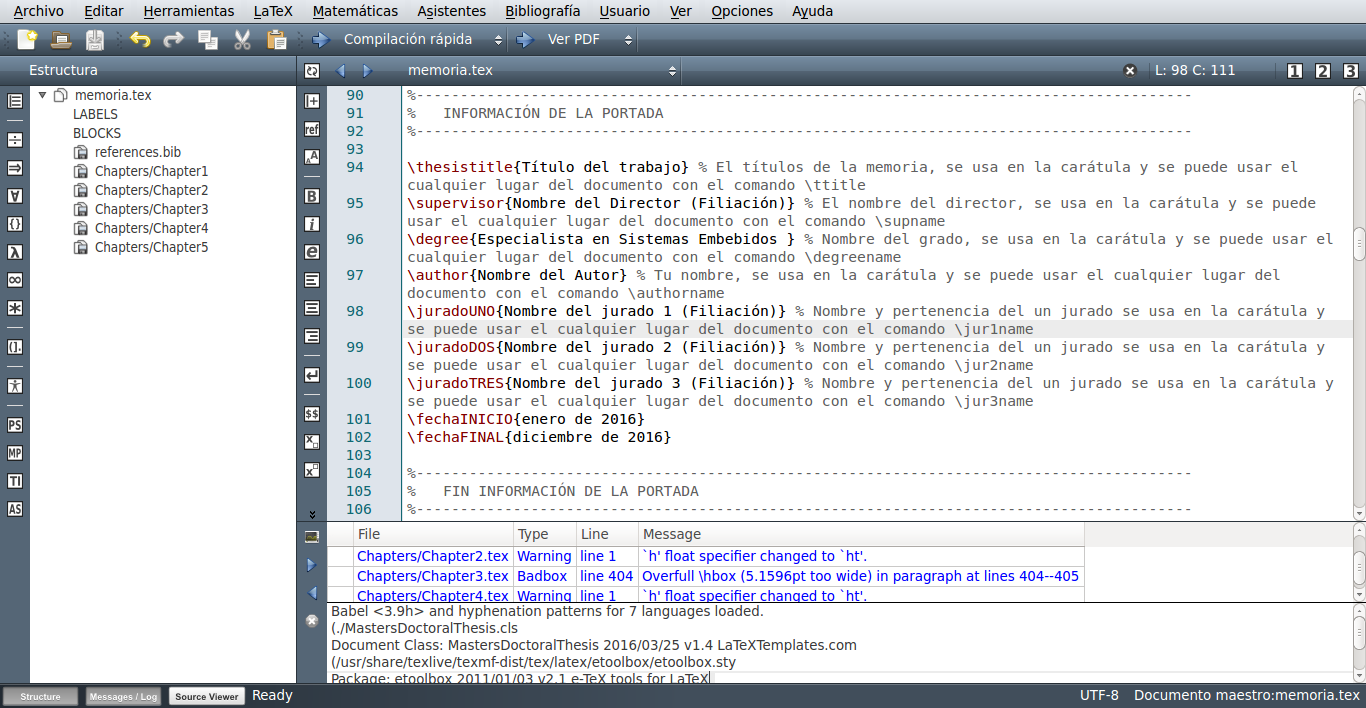
\includegraphics[width=.5\textwidth]{./Figures/texmaker.png}
% 	\caption{Entorno de trabajo de texMaker.}
% 	\label{fig:texmaker}
% \end{figure}

% \vspace{1cm}

% Notar que existe una vista llamada Estructura a la izquierda de la interfaz que nos permite abrir desde dentro del programa los archivos individuales de los capítulos.  A la derecha se encuentra una vista con el archivo propiamente dicho para su edición. Hacia la parte inferior se encuentra una vista del log con información de los resultados de la compilación.  En esta última vista pueden aparecen advertencias o \textit{warning}, que normalmente pueden ser ignorados, y los errores que se indican en color rojo y deben resolverse para que se genere el PDF de salida.

% Recordar que el archivo que se debe compilar con PDFLaTeX es \file{memoria.tex}, si se tratara de compilar alguno de los capítulos saldría un error.  Para salvar la molestia de tener que cambiar de archivo para compilar cada vez que se realice una modificación en un capítulo, se puede definir el archivo \file{memoria.tex} como ``documento maestro'' yendo al menú opciones -> ``definir documento actual como documento maestro'', lo que permite compilar con PDFLaTeX memoria.tex directamente desde cualquier archivo que se esté modificando . Se muestra esta opción en la figura \ref{fig:docMaestro}.

% \begin{figure}[h]
% 	\centering
% 	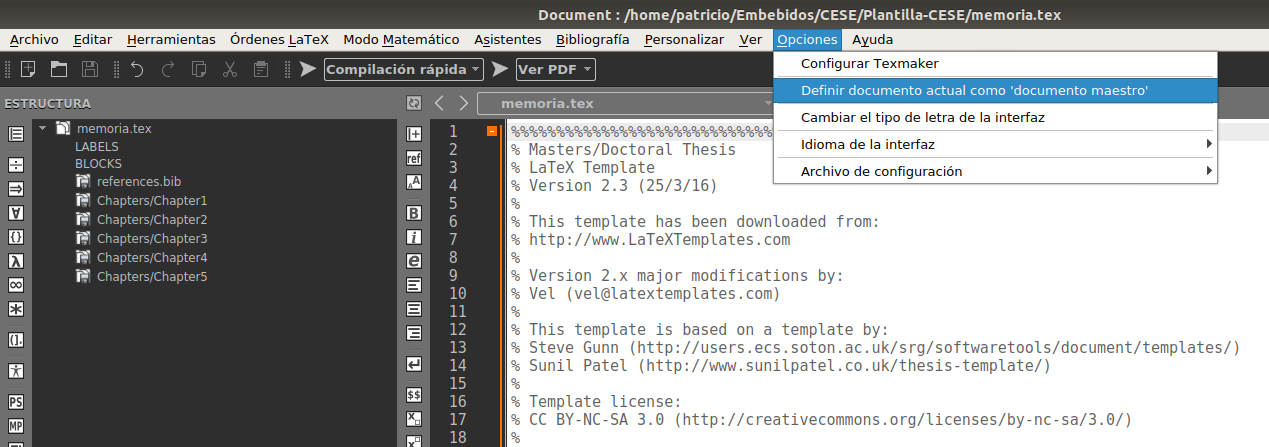
\includegraphics[width=\textwidth]{./Figures/docMaestro.png}
% 	\caption{Definir memoria.tex como documento maestro.}
% 	\label{fig:docMaestro}
% \end{figure}

% En el menú herramientas se encuentran las opciones de compilación.  Para producir un archivo PDF a partir de un archivo .tex se debe ejecutar PDFLaTeX (el shortcut es F6). Para incorporar nueva bibliografía se debe utilizar la opción BibTeX del mismo menú herramientas (el shortcut es F11).

% Notar que para actualizar las tablas de contenidos se debe ejecutar PDFLaTeX dos veces.  Esto se debe a que es necesario actualizar algunos archivos auxiliares antes de obtener el resultado final.  En forma similar, para actualizar las referencias bibliográficas se debe ejecutar primero PDFLaTeX, después BibTeX y finalmente PDFLaTeX dos veces por idénticos motivos.

% \section{Personalizando la plantilla, el archivo \file{memoria.tex}}
% \label{sec:FillingFile}

% Para personalizar la plantilla se debe incorporar la información propia en los distintos archivos \file{.tex}. 

% Primero abrir \file{memoria.tex} con TexMaker (o el editor de su preferencia). Se debe ubicar dentro del archivo el bloque de código titulado \emph{INFORMACIÓN DE LA PORTADA} donde se deben incorporar los primeros datos personales con los que se construirá automáticamente la portada.


% %----------------------------------------------------------------------------------------

% \section{El código del archivo \file{memoria.tex} explicado}

% El archivo \file{memoria.tex} contiene la estructura del documento y es el archivo de mayor jerarquía de la memoria.  Podría ser equiparable a la función \emph{main()} de un programa en C, o mejor dicho al archivo fuente .c donde se encuentra definida la función main().

% La estructura básica de cualquier documento de \LaTeX{} comienza con la definición de clase del documento, es seguida por un preámbulo donde se pueden agregar funcionalidades con el uso de \texttt{paquetes} (equiparables a bibliotecas de C), y finalmente, termina con el cuerpo del documento, donde irá el contenido de la memoria.

% \lstset{%
%   basicstyle=\small\ttfamily,
%   language=[LaTeX]{TeX}
% }

% \begin{lstlisting}
% \documentclass{article}  <- Definicion de clase
% \usepackage{listings}	 <- Preambulo

% \begin{document}	 <- Comienzo del contenido propio 
% 	Hello world!
% \end{document}
% \end{lstlisting}


% El archivo \file{memoria.tex} se encuentra densamente comentado para explicar qué páginas, secciones y elementos de formato está creando el código \LaTeX{} en cada línea. El código está dividido en bloques con nombres en mayúsculas para que resulte evidente qué es lo que hace esa porción de código en particular. Inicialmente puede parecer que hay mucho código \LaTeX{}, pero es principalmente código para dar formato a la memoria por lo que no requiere intervención del usuario de la plantilla.  Sí se deben personalizar con su información los bloques indicados como:

% \begin{itemize}
% 	\item Informacion de la memoria
% 	\item Resumen
% 	\item Agradecimientos
% 	\item Dedicatoria
% \end{itemize}

% El índice de contenidos, las listas de figura de tablas se generan en forma automática y no requieren intervención ni edición manual por parte del usuario de la plantilla. 

% En la parte final del documento se encuentran los capítulos y los apéndices.  Por defecto se incluyen los 5 capítulos propuestos que se encuentran en la carpeta /Chapters. Cada capítulo se debe escribir en un archivo .tex separado y se debe poner en la carpeta \emph{Chapters} con el nombre \file{Chapter1}, \file{Chapter2}, etc\ldots El código para incluir capítulos desde archivos externos se muestra a continuación.

% \begin{verbatim}
% 	\include{Chapters/Chapter1}
% 	\include{Chapters/Chapter2} 
% 	\include{Chapters/Chapter3}
% 	\include{Chapters/Chapter4} 
% 	\include{Chapters/Chapter5} 
% \end{verbatim}

% Los apéndices también deben escribirse en archivos .tex separados, que se deben ubicar dentro de la carpeta \emph{Appendices}. Los apéndices vienen comentados por defecto con el caracter \code{\%} y para incluirlos simplemente se debe eliminar dicho caracter.

% Finalmente, se encuentra el código para incluir la bibliografía en el documento final.  Este código tampoco debe modificarse. La metodología para trabajar las referencias bibliográficas se desarrolla en la sección \ref{sec:biblio}.
% %----------------------------------------------------------------------------------------

% \section{Bibliografía}
% \label{sec:biblio}

% Las opciones de formato de la bibliografía se controlan a través del paquete de latex \option{biblatex} que se incluye en la memoria en el archivo memoria.tex.  Estas opciones determinan cómo se generan las citas bibliográficas en el cuerpo del documento y cómo se genera la bibliografía al final de la memoria.

% En el preámbulo se puede encontrar el código que incluye el paquete biblatex, que no requiere ninguna modificación del usuario de la plantilla, y que contiene las siguientes opciones:

% \begin{lstlisting}
% \usepackage[backend=bibtex,
% 	natbib=true, 
% 	style=numeric, 
% 	sorting=none]
% {biblatex}
% \end{lstlisting}

% En el archivo \file{reference.bib} se encuentran las referencias bibliográficas que se pueden citar en el documento.  Para incorporar una nueva cita al documento lo primero es agregarla en este archivo con todos los campos necesario.  Todas las entradas bibliográficas comienzan con $@$ y una palabra que define el formato de la entrada.  Para cada formato existen campos obligatorios que deben completarse. No importa el orden en que las entradas estén definidas en el archivo .bib.  Tampoco es importante el orden en que estén definidos los campos de una entrada bibliográfica. A continuación se muestran algunos ejemplos:

% \begin{lstlisting}
% @ARTICLE{ARTICLE:1,
%     AUTHOR="John Doe",
%     TITLE="Title",
%     JOURNAL="Journal",
%     YEAR="2017",
% }
% \end{lstlisting}


% \begin{lstlisting}
% @BOOK{BOOK:1,
%     AUTHOR="John Doe",
%     TITLE="The Book without Title",
%     PUBLISHER="Dummy Publisher",
%     YEAR="2100",
% }
% \end{lstlisting}


% \begin{lstlisting}
% @INBOOK{BOOK:2,
%     AUTHOR="John Doe",
%     TITLE="The Book without Title",
%     PUBLISHER="Dummy Publisher",
%     YEAR="2100",
%     PAGES="100-200",
% }
% \end{lstlisting}


% \begin{lstlisting}
% @MISC{WEBSITE:1,
%     HOWPUBLISHED = "\url{http://example.com}",
%     AUTHOR = "Intel",
%     TITLE = "Example Website",
%     MONTH = "12",
%     YEAR = "1988",
%     URLDATE = {2012-11-26}
% }
% \end{lstlisting}

% Se debe notar que los nombres \emph{ARTICLE:1}, \emph{BOOK:1}, \emph{BOOK:2} y \emph{WEBSITE:1} son nombres de fantasía que le sirve al autor del documento para identificar la entrada. En este sentido, se podrían reemplazar por cualquier otro nombre.  Tampoco es necesario poner : seguido de un número, en los ejemplos sólo se incluye como un posible estilo para identificar las entradas.

% La entradas se citan en el documento con el comando: 

% \begin{verbatim}
% \citep{nombre_de_la_entrada}
% \end{verbatim}

% Y cuando se usan, se muestran así: \citep{ARTICLE:1}, \citep{BOOK:1}, \citep{BOOK:2}, \citep{WEBSITE:1}.  Notar cómo se conforma la sección Bibliografía al final del documento.

% Finalmente y como se mencionó en la subsección \ref{subsec:configurando}, para actualizar las referencias bibliográficas tanto en la sección bibliografía como las citas en el cuerpo del documento, se deben ejecutar las herramientas de compilación PDFLaTeX, BibTeX, PDFLaTeX, PDFLaTeX, en ese orden.  Este procedimiento debería resolver cualquier mensaje "Citation xxxxx on page x undefined".

% 	\chapter{Introducción específica} 

\label{Chapter2}

Este capítulo presenta los conceptos y componentes centrales que sustentan el trabajo. Se introducen los sistemas de recomendación y sus enfoques principales, se describen las fuentes de información empleadas y se detallan las plataformas y herramientas utilizadas para el procesamiento de datos, el modelado y la gestión de experimentos, que conforman la base tecnológica de la solución propuesta.
%----------------------------------------------------------------------------------------

\section{Sistemas de recomendación}

Los sistemas de recomendación constituyen una de las aplicaciones más extendidas de la inteligencia artificial \cite{BOOK:Ricci2015,ARTICLE:Adomavicius2005}, con un papel central en la reducción de la sobrecarga de información y en la optimización de decisiones de consumo. Su finalidad es generar sugerencias personalizadas que se ajusten a las características de cada cliente, lo que incrementa la relevancia de los productos ofrecidos y mejora la experiencia general de interacción con la empresa.

\subsection{Funcionamiento de los sistemas de recomendación}

El eje central del enfoque consiste en identificar relaciones de similitud entre productos, clientes o interacciones \cite{BOOK:Ricci2015}. Estas relaciones pueden establecerse desde diferentes perspectivas. En primer lugar, es posible medir la similitud entre productos, lo que permite agrupar aquellos que suelen adquirirse en conjunto o que comparten atributos comunes. En segundo lugar, puede analizarse la similitud entre clientes, de modo que las preferencias observadas en un grupo con comportamientos semejantes permitan anticipar las elecciones de otros con perfiles cercanos. Por último, también resulta clave la similitud entre interacciones, que considera el historial de comportamientos de un cliente, como sus compras o búsquedas, para anticipar futuras decisiones.

Un ejemplo ilustrativo, representado en la figura \ref{fig:ejemploSimilitud}, puede plantearse en la industria de bebidas. Supongamos que cada marca de cerveza se representa como un vector en un espacio definido por atributos, como \texttt{tradicional versus innovador} y \texttt{masivo versus \textit{premium}}. En ese espacio, una lager clásica de gran consumo quedaría ubicada cerca de otras variedades tradicionales y de alcance masivo, mientras que una IPA artesanal o una edición limitada se situarían en la región asociada a lo \textit{premium} e innovador. El sistema de recomendación aprovecha esta representación para calcular distancias o similaridades entre productos. Si un cliente suele elegir artículos situados en torno al cuadrante de \texttt{\textit{premium}–tradicional}, el modelo infiere que probablemente muestre interés por otras marcas que ocupan posiciones cercanas en ese mismo espacio vectorial. De esta manera, la proximidad entre vectores se convierte en un indicador de afinidad, que guía la generación de recomendaciones personalizadas.

\begin{figure}[htpb]
	\centering
	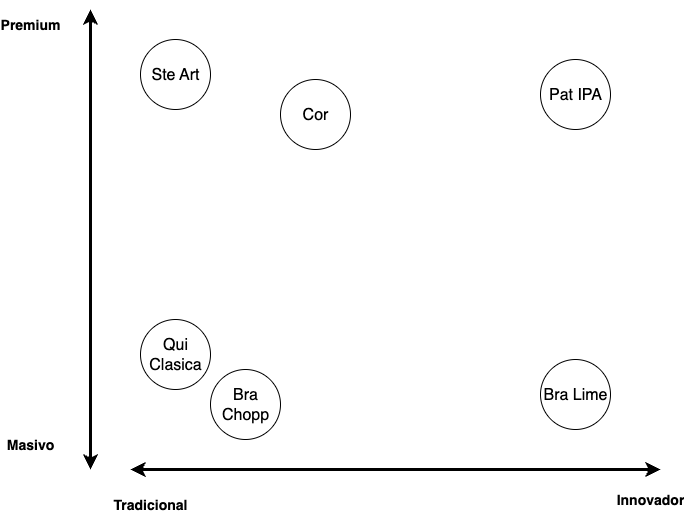
\includegraphics[scale=.4]{./Figures/ejemploSimilitud.png}
	\caption{Ejemplo de representación de marcas de cerveza en un espacio de atributos.}
	\label{fig:ejemploSimilitud}
\end{figure}

\subsection{Tipos de \textit{feedback}}

El tipo de información disponible para alimentar un sistema de recomendación también es determinante. Se distinguen dos formas principales de retroalimentación \cite{ARTICLE:Hu2008}. La retroalimentación explícita consiste en la valoración directa que realizan los clientes sobre los productos, como calificaciones numéricas, encuestas o reseñas. La retroalimentación implícita, en cambio, se infiere del comportamiento de los clientes, ya sea a través de sus compras, búsquedas o interacciones digitales. En el ámbito B2B, donde no es común que los clientes asignen calificaciones explícitas, predominan las señales implícitas, lo que plantea desafíos adicionales para la construcción de modelos precisos.

\subsection{Filtrado colaborativo}

El filtrado colaborativo se apoya en la hipótesis de que usuarios similares tienden a preferir ítems similares, lo que puede abordarse mediante enfoques \textit{user-based} o \textit{item-based} \cite{ARTICLE:Sarwar2001}. Su implementación moderna se basa en factorización matricial \cite{ARTICLE:Koren2009}.

En la modalidad \textit{user-based}, se recomienda a un cliente productos que fueron consumidos por otros con patrones de compra semejantes. En la modalidad \textit{item-based}, se priorizan productos que suelen aparecer en conjunto en los historiales de distintos clientes. 

El filtrado colaborativo suele implementarse mediante técnicas de factorización matricial. Dado un conjunto de $m$ usuarios y $n$ productos, se construye una matriz de interacciones $R \in \mathbb{R}^{m \times n}$, donde cada celda refleja el vínculo entre un cliente y un producto. El objetivo consiste en aproximar esta matriz como el producto de dos matrices de menor dimensión, como se puede observar en \ref{eq:factorizacion}.

\begin{equation}
\label{eq:factorizacion}
R \approx U \cdot V^T
\end{equation}

donde $U \in \mathbb{R}^{m \times k}$ representa a los usuarios en un espacio latente de dimensión $k$, y $V \in \mathbb{R}^{n \times k}$ representa a los ítems en ese mismo espacio. La predicción de la afinidad del usuario $i$ con el ítem $j$ se calcula en \ref{eq:prediccion_cf} como el producto escalar entre los vectores latentes correspondientes.

\begin{equation}
\label{eq:prediccion_cf}
\hat{r}_{ij} = u_i \cdot v_j^T
\end{equation}

Este modelo permite capturar relaciones complejas entre clientes y productos a partir de información implícita, aunque presenta limitaciones frente al problema del arranque en frío, cuando no existe historial suficiente de interacciones.

\subsection{Sistemas basados en contenido}

Otro enfoque ampliamente utilizado es el de los sistemas basados en contenido, que centran la recomendación en las características de los productos y en el perfil de cada cliente \cite{ARTICLE:Pazzani2007}. En este caso, se representa a cada producto por un vector de atributos y se construye un perfil para cada cliente que refleja la importancia relativa de esos atributos en función de sus elecciones pasadas. La predicción de relevancia para recomendar un producto $j$ a un cliente $i$ puede expresarse de manera simplificada como en \ref{eq:prediccion_cb}.

\begin{equation}
\label{eq:prediccion_cb}
\hat{r}_{ij} = w_i \cdot x_j
\end{equation}

donde $x_j$ es el vector de atributos del producto y $w_i$ representa el perfil del cliente. Este método permite recomendar productos nuevos o poco frecuentes siempre que exista información suficiente sobre sus atributos, lo que lo convierte en un complemento natural del filtrado colaborativo.

%----------------------------------------------------------------------------------------

\section{Fuentes de información}


%  -- Muy especifico sobre el trabajo, lo dejo para el cap 3 --
% El desarrollo del sistema de recomendación se apoya en un conjunto diverso de datos que, en su integración, permiten construir una representación enriquecida de la relación cliente–producto. Estas fuentes incluyen información transaccional, eventos de interacción en la aplicación BEES y atributos contextuales de clientes y productos. En conjunto, estos elementos aportan evidencia implícita de interés y afinidad, y constituyen la base para la estimación de scores personalizados.

% Los datos transaccionales reflejan las compras efectivamente realizadas por cada cliente. Dentro de esta categoría se consideran las siguientes variables: volumen adquirido por producto, frecuencia de compra, recencia de la última operación, monetización total y participación relativa de cada producto en el mix de compras del cliente. Estas medidas permiten capturar el grado de preferencia y relevancia actual de cada artículo en la cartera de cada punto de venta.

% A su vez, se incorporan eventos de comportamiento generados en la aplicación BEES, los cuales funcionan como señales implícitas de interés. Entre ellos se incluyen agregados y remociones de productos del carrito, visualizaciones de fichas de producto, búsquedas realizadas, calificaciones o reseñas, y clics en promociones. Estos registros aportan información complementaria sobre el proceso de consideración del cliente, incluso en los casos en los que no se concreta una transacción.

% La caracterización se completa con variables de contexto asociadas tanto a clientes como a productos. Del lado del cliente, se integran atributos como el canal comercial y la ubicación geográfica. Del lado del producto, se consideran propiedades como marca, segmento, calibre y participación de mercado. Este conjunto de información contextual permite capturar heterogeneidades relevantes que condicionan la relación de afinidad.

% De esta forma, la combinación de datos transaccionales, eventos digitales y atributos contextuales permite construir una representación integral de las interacciones cliente–producto, sobre la cual se sustenta el modelado de afinidad.

El funcionamiento de los sistemas de recomendación se apoya en diversas fuentes de información \cite{BOOK:Ricci2015,ARTICLE:Adomavicius2005} que, al combinarse, permiten construir una representación más completa de la relación entre usuarios y productos. Estas fuentes pueden clasificarse en tres grandes categorías: datos transaccionales, señales de interacción y atributos contextuales.

Los datos transaccionales reflejan las operaciones efectivamente realizadas, como compras, alquileres o reproducciones. Constituyen una evidencia directa de preferencia, ya que expresan decisiones concretas de los usuarios respecto a determinados productos o servicios.

Las señales de interacción incluyen registros de comportamiento que no necesariamente culminan en una transacción, pero que aportan información implícita de interés. Las señales implícitas, como visualizaciones o clics, resultan especialmente valiosas en contextos digitales \cite{ARTICLE:Hu2008,ARTICLE:Covington2016}. Ejemplos de este tipo de datos son las visualizaciones de fichas de producto, las búsquedas realizadas en una plataforma, las adiciones y eliminaciones en un carrito digital o las calificaciones otorgadas. Estas interacciones permiten identificar patrones de consideración más allá de la compra final.

Finalmente, los atributos contextuales corresponden a características adicionales tanto de los usuarios como de los productos. Del lado de los usuarios, se pueden incluir variables demográficas, geográficas o vinculadas al canal de consumo. Del lado de los productos, se consideran atributos como categoría, marca, segmento o características técnicas. Este conjunto de información enriquece la representación de afinidad, al capturar heterogeneidades que condicionan las recomendaciones.

De esta forma, la integración de datos transaccionales, señales de interacción y atributos contextuales constituye la base informativa sobre la cual se construyen los diferentes enfoques de recomendación. La disponibilidad y calidad de estas fuentes son determinantes para el desempeño de los modelos y para la capacidad de generar sugerencias precisas y relevantes.


%----------------------------------------------------------------------------------------

\section{Herramientas utilizadas}

%  -- Muy especifico sobre el trabajo, lo dejo para el cap 3 --
% El desarrollo del trabajo se apoyó en un conjunto de herramientas tecnológicas que permitieron gestionar de manera eficiente el ciclo de vida completo del sistema de recomendación, desde la preparación de datos hasta el despliegue de modelos.

% En primer lugar, se utilizó la plataforma Databricks, que combina capacidades de procesamiento distribuido con un entorno colaborativo para el análisis de datos. Databricks permitió integrar múltiples fuentes, realizar transformaciones a gran escala con \texttt{PySpark} y organizar flujos de trabajo de forma reproducible y escalable. Su uso facilitó tanto la exploración inicial como la construcción de pipelines de ingeniería de atributos.A

% En segundo lugar, se empleó \texttt{MLflow} como herramienta de gestión del ciclo de vida de modelos. A través de esta plataforma se registraron experimentos, parámetros, métricas y versiones de modelos, lo que aseguró trazabilidad y comparabilidad entre distintos enfoques. Asimismo, se utilizaron las funcionalidades de almacenamiento y versionado de artefactos para garantizar la reproducibilidad de resultados y la posibilidad de mantener un repositorio consolidado de modelos entrenados.

% El trabajo también se apoyó en bibliotecas de aprendizaje automático ampliamente utilizadas en la comunidad científica y profesional. Entre ellas se destaca \texttt{MLlib}, utilizada para implementar la factorización matricial con \texttt{ALS}. Asimismo, se empleó \texttt{LightFM} para el desarrollo de modelos híbridos de filtrado colaborativo. Finalmente, se incorporó \texttt{PyTorch} como entorno de \textit{deep learning}, lo que permitió construir arquitecturas más complejas capaces de capturar patrones no lineales en las interacciones cliente–producto. Adicionalmente, se utilizaron bibliotecas de visualización como \texttt{matplotlib} y \texttt{seaborn} para generar representaciones gráficas que complementaron el análisis exploratorio y la evaluación de resultados.

% Finalmente, se recurrió a entornos de control de versiones y colaboración, en particular \texttt{GitHub}, lo que permitió organizar el código en repositorios estructurados, registrar cambios de manera sistemática y facilitar la integración de componentes en distintas fases del trabajo.

% En conjunto, estas herramientas proporcionaron una infraestructura sólida para desarrollar, evaluar y documentar el sistema de recomendación, lo que aseguró tanto la calidad técnica como la escalabilidad del enfoque implementado.

% --- MUY GENERICO ---

% El desarrollo de sistemas de recomendación requiere una infraestructura tecnológica que permita gestionar de manera eficiente el ciclo de vida completo de los modelos, desde la preparación de datos hasta su despliegue en entornos productivos. Para ello, se emplean plataformas y herramientas que integran capacidades de procesamiento, experimentación y gestión colaborativa.

% En primer lugar, las plataformas de procesamiento distribuido resultan fundamentales para manipular grandes volúmenes de datos y realizar transformaciones a escala. Estas soluciones suelen combinar entornos colaborativos con motores de cálculo paralelizado, lo que facilita tanto la exploración inicial como la construcción de flujos de trabajo reproducibles.

% En segundo lugar, los sistemas de gestión del ciclo de vida de modelos (MLOps) permiten registrar experimentos, parámetros, métricas y versiones de modelos. Estas herramientas aseguran trazabilidad, reproducibilidad y comparabilidad entre diferentes enfoques, además de posibilitar el almacenamiento y versionado de artefactos.

% Adicionalmente, se utilizan bibliotecas de aprendizaje automático y profundo que constituyen estándares en la comunidad científica y profesional. Entre ellas se destacan entornos para la implementación de algoritmos clásicos de recomendación, bibliotecas para modelos híbridos y marcos de trabajo de deep learning que permiten capturar patrones complejos en las interacciones entre clientes y productos. Estas soluciones suelen complementarse con bibliotecas de visualización orientadas a generar representaciones gráficas que apoyen el análisis exploratorio y la evaluación de resultados.

% Finalmente, las plataformas de control de versiones y colaboración cumplen un rol central en la organización del código, el registro de cambios y la integración de componentes en distintas fases del desarrollo. Estas herramientas permiten estructurar repositorios, asegurar calidad en los procesos de desarrollo y facilitar la coordinación entre equipos.

% En conjunto, este ecosistema de plataformas y bibliotecas constituye la base tecnológica sobre la cual se implementan los sistemas de recomendación modernos, garantizando tanto la calidad técnica como la escalabilidad de las soluciones.

El desarrollo de este trabajo se apoyó en un conjunto de herramientas tecnológicas que facilitaron la gestión integral del ciclo de vida del sistema de recomendación. A continuación, se detallan las principales plataformas, bibliotecas y entornos empleados, junto con su función específica en el proceso.

\subsection{Plataformas de procesamiento distribuido}

El procesamiento y consolidación de grandes volúmenes de información se llevó a cabo en la plataforma Databricks \cite{ARTICLE:Databricks}, que integra un entorno colaborativo con un motor de cómputo distribuido basado en Apache Spark \cite{ARTICLE:Spark2012}. Esta herramienta permitió orquestar la ingestión de datos, ejecutar transformaciones a gran escala mediante PySpark y garantizar reproducibilidad en los flujos de trabajo. El uso de Databricks resultó fundamental para integrar múltiples fuentes y preparar los insumos que alimentaron las etapas de análisis y modelado.

\subsection{Gestión del ciclo de vida de modelos}

Para la gestión del ciclo de vida de los modelos se empleó MLflow \cite{ARTICLE:MLflow2018}, plataforma que facilita el registro de experimentos, parámetros, métricas y versiones de modelos. Esta herramienta permitió mantener trazabilidad entre las distintas ejecuciones, asegurar comparabilidad de resultados y almacenar los artefactos generados (modelos entrenados y estructuras derivadas). De este modo, se consolidó un repositorio ordenado que garantizó reproducibilidad y control en la experimentación.

\subsection{Bibliotecas de aprendizaje automático y profundo}

En el desarrollo de los modelos se emplearon distintas bibliotecas que constituyen estándares en la comunidad científica y profesional. Se utilizó MLlib para implementar el filtrado colaborativo mediante factorización matricial con el algoritmo Alternating Least Squares (ALS) \cite{ARTICLE:ALS2008}, mientras que LightFM \cite{ARTICLE:LightFM2015} permitió construir un modelo híbrido que combina señales de interacción implícita con atributos de clientes y productos. Adicionalmente, se recurrió a PyTorch como entorno de deep learning para el diseño de arquitecturas neuronales capaces de capturar relaciones no lineales y complejas en los datos. 

\subsection{Bibliotecas de visualización}

Para el análisis visual y la generación de gráficos se utilizaron bibliotecas como Matplotlib \cite{ARTICLE:Matplotlib2007} y Seaborn \cite{ARTICLE:Seaborn2021}, que facilitaron la representación gráfica tanto de la información explorada como de los resultados obtenidos en las distintas fases del trabajo.

\subsection{Control de versiones y colaboración}

La organización y versionado del código se gestionaron mediante GitHub \cite{ARTICLE:GitHub}, que permitió estructurar los repositorios, registrar cambios de manera sistemática y facilitar la colaboración. El uso de esta plataforma aseguró orden en el desarrollo, trazabilidad de modificaciones y una integración eficiente de los distintos componentes del sistema.

\subsection{Consideraciones finales}

En conjunto, estas herramientas brindaron una infraestructura robusta para abordar todas las etapas del desarrollo del sistema de recomendación, desde la preparación de los datos hasta la evaluación y almacenamiento de modelos. Cabe destacar que la calidad de una implementación no depende únicamente del algoritmo utilizado, sino también de la solidez del entorno técnico que la respalda. El uso articulado de estas herramientas permitió asegurar la reproducibilidad de los resultados, la eficiencia en el manejo de datos, la trazabilidad de las decisiones y la escalabilidad del sistema desarrollado. En el contexto de una solución real, contar con esta base técnica resulta clave para garantizar tanto la calidad técnica como la posibilidad de evolución futura del sistema.

%----------------------------------------------------------------------------------------


% \section{Estilo y convenciones}
% \label{sec:ejemplo}

% \subsection{Uso de mayúscula inicial para los título de secciones}

% Si en el texto se hace alusión a diferentes partes del trabajo referirse a ellas como capítulo, sección o subsección según corresponda. Por ejemplo: ``En el capítulo \cite{Chapter1} se explica tal cosa'', o ``En la sección \cite{sec:ejemplo} se presenta lo que sea'', o ``En la subsección \cite{subsec:ejemplo} se discute otra cosa''.

% Cuando se quiere poner una lista tabulada, se hace así:

% \begin{itemize}
% 	\item Este es el primer elemento de la lista.
% 	\item Este es el segundo elemento de la lista.
% \end{itemize}

% Notar el uso de las mayúsculas y el punto al final de cada elemento.

% Si se desea poner una lista numerada el formato es este:

% \begin{enumerate}
% 	\item Este es el primer elemento de la lista.
% 	\item Este es el segundo elemento de la lista.
% \end{enumerate}

% Notar el uso de las mayúsculas y el punto al final de cada elemento.

% \subsection{Este es el título de una subsección}
% \label{subsec:ejemplo}

% Se recomienda no utilizar \textbf{texto en negritas} en ningún párrafo, ni tampoco texto \underline{subrayado}. En cambio sí se debe utilizar \textit{texto en itálicas} para palabras en un idioma extranjero, al menos la primera vez que aparecen en el texto. En el caso de palabras que estamos inventando se deben utilizar ``comillas'', así como también para citas textuales. Por ejemplo, un \textit{digital filter} es una especie de ``selector'' que permite separar ciertos componentes armónicos en particular.

% La escritura debe ser impersonal. Por ejemplo, no utilizar ``el diseño del firmware lo hice de acuerdo con tal principio'', sino ``el firmware fue diseñado utilizando tal principio''. 

% El trabajo es algo que al momento de escribir la memoria se supone que ya está concluido, entonces todo lo que se refiera a hacer el trabajo se narra en tiempo pasado, porque es algo que ya ocurrió. Por ejemplo, "se diseñó el firmware empleando la técnica de test driven development".

% En cambio, la memoria es algo que está vivo cada vez que el lector la lee. Por eso transcurre siempre en tiempo presente, como por ejemplo:

% ``En el presente capítulo se da una visión global sobre las distintas pruebas realizadas y los resultados obtenidos. Se explica el modo en que fueron llevados a cabo los test unitarios y las pruebas del sistema''.

% Se recomienda no utilizar una sección de glosario sino colocar la descripción de las abreviaturas como parte del mismo cuerpo del texto. Por ejemplo, RTOS (\textit{Real Time Operating System}, Sistema Operativo de Tiempo Real) o en caso de considerarlo apropiado mediante notas a pie de página.

% Si se desea indicar alguna página web utilizar el siguiente formato de referencias bibliográficas, dónde las referencias se detallan en la sección de bibliografía de la memoria, utilizado el formato establecido por IEEE en \citep{IEEE:citation}. Por ejemplo, ``el presente trabajo se basa en la plataforma EDU-CIAA-NXP \citep{CIAA}, la cual...''.

% \subsection{Figuras} 

% Al insertar figuras en la memoria se deben considerar determinadas pautas. Para empezar, usar siempre tipografía claramente legible. Luego, tener claro que \textbf{es incorrecto} escribir por ejemplo esto: ``El diseño elegido es un cuadrado, como se ve en la siguiente figura:''

% \begin{figure}[h]
% \centering
% 
\includegraphics[scale=.45]{./Figures/cuadradoAzul.png}
% \end{figure}

% La forma correcta de utilizar una figura es con referencias cruzadas, por ejemplo: ``Se eligió utilizar un cuadrado azul para el logo, como puede observarse en la figura \cite{fig:cuadradoAzul}''.

% \begin{figure}[ht]
% 	\centering
% 	
\includegraphics[scale=.45]{./Figures/cuadradoAzul.png}
% 	\caption{Ilustración del cuadrado azul que se eligió para el diseño del logo.}
% 	\label{fig:cuadradoAzul}
% \end{figure}

% El texto de las figuras debe estar siempre en español, excepto que se decida reproducir una figura original tomada de alguna referencia. En ese caso la referencia de la cual se tomó la figura debe ser indicada en el epígrafe de la figura e incluida como una nota al pie, como se ilustra en la figura \cite{fig:palabraIngles}.

% \begin{figure}[htpb]
% 	\centering
% 	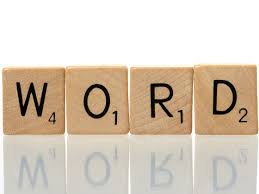
\includegraphics[scale=.3]{./Figures/word.jpeg}
% 	\caption{Imagen tomada de la página oficial del procesador\protect\footnotemark.}
% 	\label{fig:palabraIngles}
% \end{figure}

% \footnotetext{Imagen tomada de \url{https://goo.gl/images/i7C70w}}

% La figura y el epígrafe deben conformar una unidad cuyo significado principal pueda ser comprendido por el lector sin necesidad de leer el cuerpo central de la memoria. Para eso es necesario que el epígrafe sea todo lo detallado que corresponda y si en la figura se utilizan abreviaturas entonces aclarar su significado en el epígrafe o en la misma figura.



% \begin{figure}[ht]
% 	\centering
% 	
\includegraphics[scale=.37]{./Figures/questionMark.png}
% 	\caption{¿Por qué de pronto aparece esta figura?}
% 	\label{fig:questionMark}
% \end{figure}

% Nunca colocar una figura en el documento antes de hacer la primera referencia a ella, como se ilustra con la figura \cite{fig:questionMark}, porque sino el lector no comprenderá por qué de pronto aparece la figura en el documento, lo que distraerá su atención.

% Otra posibilidad es utilizar el entorno \textit{subfigure} para incluir más de una figura, como se puede ver en la figura \cite{fig:three graphs}. Notar que se pueden referenciar también las figuras internas individualmente de esta manera: \cite{fig:1de3}, \cite{fig:2de3} y \cite{fig:3de3}.
 
% \begin{figure}[!htpb]
%      \centering
%      \begin{subfigure}[b]{0.3\textwidth}
%          \centering
%          
\includegraphics[width=.65\textwidth]{./Figures/questionMark}
%          \caption{Un caption.}
%          \label{fig:1de3}
%      \end{subfigure}
%      \hfill
%      \begin{subfigure}[b]{0.3\textwidth}
%          \centering
%          
\includegraphics[width=.65\textwidth]{./Figures/questionMark}
%          \caption{Otro.}
%          \label{fig:2de3}
%      \end{subfigure}
%      \hfill
%      \begin{subfigure}[b]{0.3\textwidth}
%          \centering
%          
\includegraphics[width=.65\textwidth]{./Figures/questionMark}
%          \caption{Y otro más.}
%          \label{fig:3de3}
%      \end{subfigure}
%         \caption{Tres gráficos simples.}
%         \label{fig:three graphs}
% \end{figure}

% El código para generar las imágenes se encuentra disponible para su reutilización en el archivo \file{Chapter2.tex}.

% \subsection{Tablas}

% Para las tablas utilizar el mismo formato que para las figuras, sólo que el epígrafe se debe colocar arriba de la tabla, como se ilustra en la tabla \cite{tab:peces}. Observar que sólo algunas filas van con líneas visibles y notar el uso de las negritas para los encabezados.  La referencia se logra utilizando el comando \verb|\cite{<label>}| donde label debe estar definida dentro del entorno de la tabla.

% \begin{verbatim}
% \begin{table}[h]
% 	\centering
% 	\caption[caption corto]{caption largo más descriptivo}
% 	\begin{tabular}{l c c}    
% 		\toprule
% 		\textbf{Especie}     & \textbf{Tamaño} & \textbf{Valor}\\
% 		\midrule
% 		Amphiprion Ocellaris & 10 cm           & \$ 6.000 \\		
% 		Hepatus Blue Tang    & 15 cm           & \$ 7.000 \\
% 		Zebrasoma Xanthurus  & 12 cm           & \$ 6.800 \\
% 		\bottomrule
% 		\hline
% 	\end{tabular}
% 	\label{tab:peces}
% \end{table}
% \end{verbatim}


% \begin{table}[h]
% 	\centering
% 	\caption[caption corto]{caption largo más descriptivo.}
% 	\begin{tabular}{l c c}    
% 		\toprule
% 		\textbf{Especie} 	 & \textbf{Tamaño} 		& \textbf{Valor}  \\
% 		\midrule
% 		Amphiprion Ocellaris & 10 cm 				& \$ 6.000 \\		
% 		Hepatus Blue Tang	 & 15 cm				& \$ 7.000 \\
% 		Zebrasoma Xanthurus	 & 12 cm				& \$ 6.800 \\
% 		\bottomrule
% 		\hline
% 	\end{tabular}
% 	\label{tab:peces}
% \end{table}

% En cada capítulo se debe reiniciar el número de conteo de las figuras y las tablas, por ejemplo, figura 2.1 o tabla 2.1, pero no se debe reiniciar el conteo en cada sección. Por suerte la plantilla se encarga de esto por nosotros.

% \subsection{Ecuaciones}
% \label{sec:Ecuaciones}

% Al insertar ecuaciones en la memoria dentro de un entorno \textit{equation}, éstas se numeran en forma automática  y se pueden referir al igual que como se hace con las figuras y tablas, por ejemplo ver la ecuación \cite{eq:metric}.

% \begin{equation}
% 	\label{eq:metric}
% 	ds^2 = c^2 dt^2 \left( \frac{d\sigma^2}{1-k\sigma^2} + \sigma^2\left[ d\theta^2 + \sin^2\theta d\phi^2 \right] \right)
% \end{equation}
                                                        
% Es importante tener presente que si bien las ecuaciones pueden ser referidas por su número, también es correcto utilizar los dos puntos, como por ejemplo ``la expresión matemática que describe este comportamiento es la siguiente:''

% \begin{equation}
% 	\label{eq:schrodinger}
% 	\frac{\hbar^2}{2m}\nabla^2\Psi + V(\mathbf{r})\Psi = -i\hbar \frac{\partial\Psi}{\partial t}
% \end{equation}

% Para generar la ecuación \cite{eq:metric} se utilizó el siguiente código:

% \begin{verbatim}
% \begin{equation}
% 	\label{eq:metric}
% 	ds^2 = c^2 dt^2 \left( \frac{d\sigma^2}{1-k\sigma^2} + 
% 	\sigma^2\left[ d\theta^2 + 
% 	\sin^2\theta d\phi^2 \right] \right)
% \end{equation}
% \end{verbatim}

% Y para la ecuación \cite{eq:schrodinger}:

% \begin{verbatim}
% \begin{equation}
% 	\label{eq:schrodinger}
% 	\frac{\hbar^2}{2m}\nabla^2\Psi + V(\mathbf{r})\Psi = 
% 	-i\hbar \frac{\partial\Psi}{\partial t}
% \end{equation}

% \end{verbatim} 
% 	\chapter{Diseño e implementación} % Main chapter title

\label{Chapter3} % Change X to a consecutive number; for referencing this chapter elsewhere, use \ref{ChapterX}

Todos los capítulos deben comenzar con un breve párrafo introductorio que indique cuál es el contenido que se encontrará al leerlo.  La redacción sobre el contenido de la memoria debe hacerse en presente y todo lo referido al proyecto en pasado, siempre de modo impersonal.

\definecolor{mygreen}{rgb}{0,0.6,0}
\definecolor{mygray}{rgb}{0.5,0.5,0.5}
\definecolor{mymauve}{rgb}{0.58,0,0.82}

%%%%%%%%%%%%%%%%%%%%%%%%%%%%%%%%%%%%%%%%%%%%%%%%%%%%%%%%%%%%%%%%%%%%%%%%%%%%%
% parámetros para configurar el formato del código en los entornos lstlisting
%%%%%%%%%%%%%%%%%%%%%%%%%%%%%%%%%%%%%%%%%%%%%%%%%%%%%%%%%%%%%%%%%%%%%%%%%%%%%
\lstset{ %
  backgroundcolor=\color{white},   % choose the background color; you must add \usepackage{color} or \usepackage{xcolor}
  basicstyle=\footnotesize,        % the size of the fonts that are used for the code
  breakatwhitespace=false,         % sets if automatic breaks should only happen at whitespace
  breaklines=true,                 % sets automatic line breaking
  captionpos=b,                    % sets the caption-position to bottom
  commentstyle=\color{mygreen},    % comment style
  deletekeywords={...},            % if you want to delete keywords from the given language
  %escapeinside={\%*}{*)},          % if you want to add LaTeX within your code
  %extendedchars=true,              % lets you use non-ASCII characters; for 8-bits encodings only, does not work with UTF-8
  %frame=single,	                % adds a frame around the code
  keepspaces=true,                 % keeps spaces in text, useful for keeping indentation of code (possibly needs columns=flexible)
  keywordstyle=\color{blue},       % keyword style
  language=[ANSI]C,                % the language of the code
  %otherkeywords={*,...},           % if you want to add more keywords to the set
  numbers=left,                    % where to put the line-numbers; possible values are (none, left, right)
  numbersep=5pt,                   % how far the line-numbers are from the code
  numberstyle=\tiny\color{mygray}, % the style that is used for the line-numbers
  rulecolor=\color{black},         % if not set, the frame-color may be changed on line-breaks within not-black text (e.g. comments (green here))
  showspaces=false,                % show spaces everywhere adding particular underscores; it overrides 'showstringspaces'
  showstringspaces=false,          % underline spaces within strings only
  showtabs=false,                  % show tabs within strings adding particular underscores
  stepnumber=1,                    % the step between two line-numbers. If it's 1, each line will be numbered
  stringstyle=\color{mymauve},     % string literal style
  tabsize=2,	                   % sets default tabsize to 2 spaces
  title=\lstname,                  % show the filename of files included with \lstinputlisting; also try caption instead of title
  morecomment=[s]{/*}{*/}
}


%----------------------------------------------------------------------------------------
%	SECTION 1
%----------------------------------------------------------------------------------------
% \section{Análisis del software}
 
% La idea de esta sección es resaltar los problemas encontrados, los criterios utilizados y la justificación de las decisiones que se hayan tomado.

% Se puede agregar código o pseudocódigo dentro de un entorno lstlisting con el siguiente código:

% \begin{verbatim}
% \begin{lstlisting}[caption= "un epígrafe descriptivo"]
% 	las líneas de código irían aquí...
% \end{lstlisting}
% \end{verbatim}

% A modo de ejemplo:

% \begin{lstlisting}[label=cod:vControl,caption=Pseudocódigo del lazo principal de control.]  % Start your code-block

% #define MAX_SENSOR_NUMBER 3
% #define MAX_ALARM_NUMBER  6
% #define MAX_ACTUATOR_NUMBER 6

% uint32_t sensorValue[MAX_SENSOR_NUMBER];		
% FunctionalState alarmControl[MAX_ALARM_NUMBER];	//ENABLE or DISABLE
% state_t alarmState[MAX_ALARM_NUMBER];						//ON or OFF
% state_t actuatorState[MAX_ACTUATOR_NUMBER];			//ON or OFF

% void vControl() {

% 	initGlobalVariables();
	
% 	period = 500 ms;
		
% 	while(1) {

% 		ticks = xTaskGetTickCount();
		
% 		updateSensors();
		
% 		updateAlarms();
		
% 		controlActuators();
		
% 		vTaskDelayUntil(&ticks, period);
% 	}
% }
% \end{lstlisting}




% 	% Chapter Template

\chapter{Ensayos y resultados} % Main chapter title

\label{Chapter4} % Change X to a consecutive number; for referencing this chapter elsewhere, use \ref{ChapterX}
Todos los capítulos deben comenzar con un breve párrafo introductorio que indique cuál es el contenido que se encontrará al leerlo.  La redacción sobre el contenido de la memoria debe hacerse en presente y todo lo referido al proyecto en pasado, siempre de modo impersonal.

%----------------------------------------------------------------------------------------
%	SECTION 1
%----------------------------------------------------------------------------------------

% \section{Pruebas funcionales del hardware}
% \label{sec:pruebasHW}

% La idea de esta sección es explicar cómo se hicieron los ensayos, qué resultados se obtuvieron y analizarlos.
 
% 	% Chapter Template

\chapter{Conclusiones} % Main chapter title

\label{Chapter5} % Change X to a consecutive number; for referencing this chapter elsewhere, use \ref{ChapterX}
Todos los capítulos deben comenzar con un breve párrafo introductorio que indique cuál es el contenido que se encontrará al leerlo.  La redacción sobre el contenido de la memoria debe hacerse en presente y todo lo referido al proyecto en pasado, siempre de modo impersonal.


%----------------------------------------------------------------------------------------

%----------------------------------------------------------------------------------------
%	SECTION 1
%----------------------------------------------------------------------------------------

% \section{Conclusiones generales }

% La idea de esta sección es resaltar cuáles son los principales aportes del trabajo realizado y cómo se podría continuar. Debe ser especialmente breve y concisa. Es buena idea usar un listado para enumerar los logros obtenidos.

% En esta sección no se deben incluir ni tablas ni gráficos.

% Algunas preguntas que pueden servir para completar este capítulo:

% \begin{itemize}
% \item ¿Cuál es el grado de cumplimiento de los requerimientos?
% \item ¿Cuán fielmente se puedo seguir la planificación original (cronograma incluido)?
% \item ¿Se manifestó algunos de los riesgos identificados en la planificación? ¿Fue efectivo el plan de mitigación? ¿Se debió aplicar alguna otra acción no contemplada previamente?
% \item Si se debieron hacer modificaciones a lo planificado ¿Cuáles fueron las causas y los efectos?
% \item ¿Qué técnicas resultaron útiles para el desarrollo del proyecto y cuáles no tanto?
% \end{itemize}


% %----------------------------------------------------------------------------------------
% %	SECTION 2
% %----------------------------------------------------------------------------------------
% \section{Próximos pasos}

% Acá se indica cómo se podría continuar el trabajo más adelante.
 
% \end{verbatim}

% Los apéndices también deben escribirse en archivos .tex separados, que se deben ubicar dentro de la carpeta \emph{Appendices}. Los apéndices vienen comentados por defecto con el caracter \code{\%} y para incluirlos simplemente se debe eliminar dicho caracter.

% Finalmente, se encuentra el código para incluir la bibliografía en el documento final.  Este código tampoco debe modificarse. La metodología para trabajar las referencias bibliográficas se desarrolla en la sección \ref{sec:biblio}.
% %----------------------------------------------------------------------------------------

% \section{Bibliografía}
% \label{sec:biblio}

% Las opciones de formato de la bibliografía se controlan a través del paquete de latex \option{biblatex} que se incluye en la memoria en el archivo memoria.tex.  Estas opciones determinan cómo se generan las citas bibliográficas en el cuerpo del documento y cómo se genera la bibliografía al final de la memoria.

% En el preámbulo se puede encontrar el código que incluye el paquete biblatex, que no requiere ninguna modificación del usuario de la plantilla, y que contiene las siguientes opciones:

% \begin{lstlisting}
% \usepackage[backend=bibtex,
% 	natbib=true, 
% 	style=numeric, 
% 	sorting=none]
% {biblatex}
% \end{lstlisting}

% En el archivo \file{reference.bib} se encuentran las referencias bibliográficas que se pueden citar en el documento.  Para incorporar una nueva cita al documento lo primero es agregarla en este archivo con todos los campos necesario.  Todas las entradas bibliográficas comienzan con $@$ y una palabra que define el formato de la entrada.  Para cada formato existen campos obligatorios que deben completarse. No importa el orden en que las entradas estén definidas en el archivo .bib.  Tampoco es importante el orden en que estén definidos los campos de una entrada bibliográfica. A continuación se muestran algunos ejemplos:

% \begin{lstlisting}
% @ARTICLE{ARTICLE:1,
%     AUTHOR="John Doe",
%     TITLE="Title",
%     JOURNAL="Journal",
%     YEAR="2017",
% }
% \end{lstlisting}


% \begin{lstlisting}
% @BOOK{BOOK:1,
%     AUTHOR="John Doe",
%     TITLE="The Book without Title",
%     PUBLISHER="Dummy Publisher",
%     YEAR="2100",
% }
% \end{lstlisting}


% \begin{lstlisting}
% @INBOOK{BOOK:2,
%     AUTHOR="John Doe",
%     TITLE="The Book without Title",
%     PUBLISHER="Dummy Publisher",
%     YEAR="2100",
%     PAGES="100-200",
% }
% \end{lstlisting}


% \begin{lstlisting}
% @MISC{WEBSITE:1,
%     HOWPUBLISHED = "\url{http://example.com}",
%     AUTHOR = "Intel",
%     TITLE = "Example Website",
%     MONTH = "12",
%     YEAR = "1988",
%     URLDATE = {2012-11-26}
% }
% \end{lstlisting}

% Se debe notar que los nombres \emph{ARTICLE:1}, \emph{BOOK:1}, \emph{BOOK:2} y \emph{WEBSITE:1} son nombres de fantasía que le sirve al autor del documento para identificar la entrada. En este sentido, se podrían reemplazar por cualquier otro nombre.  Tampoco es necesario poner : seguido de un número, en los ejemplos sólo se incluye como un posible estilo para identificar las entradas.

% La entradas se citan en el documento con el comando: 

% \begin{verbatim}
% \citep{nombre_de_la_entrada}
% \end{verbatim}

% Y cuando se usan, se muestran así: \citep{ARTICLE:1}, \citep{BOOK:1}, \citep{BOOK:2}, \citep{WEBSITE:1}.  Notar cómo se conforma la sección Bibliografía al final del documento.

% Finalmente y como se mencionó en la subsección \ref{subsec:configurando}, para actualizar las referencias bibliográficas tanto en la sección bibliografía como las citas en el cuerpo del documento, se deben ejecutar las herramientas de compilación PDFLaTeX, BibTeX, PDFLaTeX, PDFLaTeX, en ese orden.  Este procedimiento debería resolver cualquier mensaje "Citation xxxxx on page x undefined".

% 	\chapter{Introducción específica} 

\label{Chapter2}

Este capítulo presenta los conceptos y componentes centrales que sustentan el trabajo. Se introducen los sistemas de recomendación y sus enfoques principales, se describen las fuentes de información empleadas y se detallan las plataformas y herramientas utilizadas para el procesamiento de datos, el modelado y la gestión de experimentos, que conforman la base tecnológica de la solución propuesta.
%----------------------------------------------------------------------------------------

\section{Sistemas de recomendación}

Los sistemas de recomendación constituyen una de las aplicaciones más extendidas de la inteligencia artificial \cite{BOOK:Ricci2015,ARTICLE:Adomavicius2005}, con un papel central en la reducción de la sobrecarga de información y en la optimización de decisiones de consumo. Su finalidad es generar sugerencias personalizadas que se ajusten a las características de cada cliente, lo que incrementa la relevancia de los productos ofrecidos y mejora la experiencia general de interacción con la empresa.

\subsection{Funcionamiento de los sistemas de recomendación}

El eje central del enfoque consiste en identificar relaciones de similitud entre productos, clientes o interacciones \cite{BOOK:Ricci2015}. Estas relaciones pueden establecerse desde diferentes perspectivas. En primer lugar, es posible medir la similitud entre productos, lo que permite agrupar aquellos que suelen adquirirse en conjunto o que comparten atributos comunes. En segundo lugar, puede analizarse la similitud entre clientes, de modo que las preferencias observadas en un grupo con comportamientos semejantes permitan anticipar las elecciones de otros con perfiles cercanos. Por último, también resulta clave la similitud entre interacciones, que considera el historial de comportamientos de un cliente, como sus compras o búsquedas, para anticipar futuras decisiones.

Un ejemplo ilustrativo, representado en la figura \ref{fig:ejemploSimilitud}, puede plantearse en la industria de bebidas. Supongamos que cada marca de cerveza se representa como un vector en un espacio definido por atributos, como \texttt{tradicional versus innovador} y \texttt{masivo versus \textit{premium}}. En ese espacio, una lager clásica de gran consumo quedaría ubicada cerca de otras variedades tradicionales y de alcance masivo, mientras que una IPA artesanal o una edición limitada se situarían en la región asociada a lo \textit{premium} e innovador. El sistema de recomendación aprovecha esta representación para calcular distancias o similaridades entre productos. Si un cliente suele elegir artículos situados en torno al cuadrante de \texttt{\textit{premium}–tradicional}, el modelo infiere que probablemente muestre interés por otras marcas que ocupan posiciones cercanas en ese mismo espacio vectorial. De esta manera, la proximidad entre vectores se convierte en un indicador de afinidad, que guía la generación de recomendaciones personalizadas.

\begin{figure}[htpb]
	\centering
	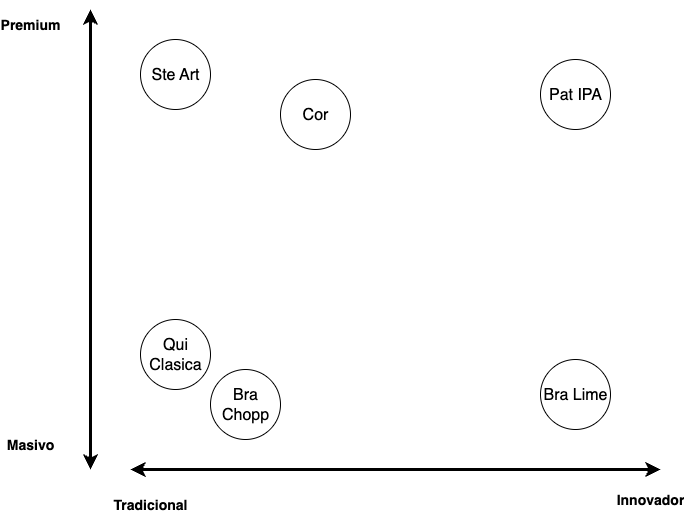
\includegraphics[scale=.4]{./Figures/ejemploSimilitud.png}
	\caption{Ejemplo de representación de marcas de cerveza en un espacio de atributos.}
	\label{fig:ejemploSimilitud}
\end{figure}

\subsection{Tipos de \textit{feedback}}

El tipo de información disponible para alimentar un sistema de recomendación también es determinante. Se distinguen dos formas principales de retroalimentación \cite{ARTICLE:Hu2008}. La retroalimentación explícita consiste en la valoración directa que realizan los clientes sobre los productos, como calificaciones numéricas, encuestas o reseñas. La retroalimentación implícita, en cambio, se infiere del comportamiento de los clientes, ya sea a través de sus compras, búsquedas o interacciones digitales. En el ámbito B2B, donde no es común que los clientes asignen calificaciones explícitas, predominan las señales implícitas, lo que plantea desafíos adicionales para la construcción de modelos precisos.

\subsection{Filtrado colaborativo}

El filtrado colaborativo se apoya en la hipótesis de que usuarios similares tienden a preferir ítems similares, lo que puede abordarse mediante enfoques \textit{user-based} o \textit{item-based} \cite{ARTICLE:Sarwar2001}. Su implementación moderna se basa en factorización matricial \cite{ARTICLE:Koren2009}.

En la modalidad \textit{user-based}, se recomienda a un cliente productos que fueron consumidos por otros con patrones de compra semejantes. En la modalidad \textit{item-based}, se priorizan productos que suelen aparecer en conjunto en los historiales de distintos clientes. 

El filtrado colaborativo suele implementarse mediante técnicas de factorización matricial. Dado un conjunto de $m$ usuarios y $n$ productos, se construye una matriz de interacciones $R \in \mathbb{R}^{m \times n}$, donde cada celda refleja el vínculo entre un cliente y un producto. El objetivo consiste en aproximar esta matriz como el producto de dos matrices de menor dimensión, como se puede observar en \ref{eq:factorizacion}.

\begin{equation}
\label{eq:factorizacion}
R \approx U \cdot V^T
\end{equation}

donde $U \in \mathbb{R}^{m \times k}$ representa a los usuarios en un espacio latente de dimensión $k$, y $V \in \mathbb{R}^{n \times k}$ representa a los ítems en ese mismo espacio. La predicción de la afinidad del usuario $i$ con el ítem $j$ se calcula en \ref{eq:prediccion_cf} como el producto escalar entre los vectores latentes correspondientes.

\begin{equation}
\label{eq:prediccion_cf}
\hat{r}_{ij} = u_i \cdot v_j^T
\end{equation}

Este modelo permite capturar relaciones complejas entre clientes y productos a partir de información implícita, aunque presenta limitaciones frente al problema del arranque en frío, cuando no existe historial suficiente de interacciones.

\subsection{Sistemas basados en contenido}

Otro enfoque ampliamente utilizado es el de los sistemas basados en contenido, que centran la recomendación en las características de los productos y en el perfil de cada cliente \cite{ARTICLE:Pazzani2007}. En este caso, se representa a cada producto por un vector de atributos y se construye un perfil para cada cliente que refleja la importancia relativa de esos atributos en función de sus elecciones pasadas. La predicción de relevancia para recomendar un producto $j$ a un cliente $i$ puede expresarse de manera simplificada como en \ref{eq:prediccion_cb}.

\begin{equation}
\label{eq:prediccion_cb}
\hat{r}_{ij} = w_i \cdot x_j
\end{equation}

donde $x_j$ es el vector de atributos del producto y $w_i$ representa el perfil del cliente. Este método permite recomendar productos nuevos o poco frecuentes siempre que exista información suficiente sobre sus atributos, lo que lo convierte en un complemento natural del filtrado colaborativo.

%----------------------------------------------------------------------------------------

\section{Fuentes de información}


%  -- Muy especifico sobre el trabajo, lo dejo para el cap 3 --
% El desarrollo del sistema de recomendación se apoya en un conjunto diverso de datos que, en su integración, permiten construir una representación enriquecida de la relación cliente–producto. Estas fuentes incluyen información transaccional, eventos de interacción en la aplicación BEES y atributos contextuales de clientes y productos. En conjunto, estos elementos aportan evidencia implícita de interés y afinidad, y constituyen la base para la estimación de scores personalizados.

% Los datos transaccionales reflejan las compras efectivamente realizadas por cada cliente. Dentro de esta categoría se consideran las siguientes variables: volumen adquirido por producto, frecuencia de compra, recencia de la última operación, monetización total y participación relativa de cada producto en el mix de compras del cliente. Estas medidas permiten capturar el grado de preferencia y relevancia actual de cada artículo en la cartera de cada punto de venta.

% A su vez, se incorporan eventos de comportamiento generados en la aplicación BEES, los cuales funcionan como señales implícitas de interés. Entre ellos se incluyen agregados y remociones de productos del carrito, visualizaciones de fichas de producto, búsquedas realizadas, calificaciones o reseñas, y clics en promociones. Estos registros aportan información complementaria sobre el proceso de consideración del cliente, incluso en los casos en los que no se concreta una transacción.

% La caracterización se completa con variables de contexto asociadas tanto a clientes como a productos. Del lado del cliente, se integran atributos como el canal comercial y la ubicación geográfica. Del lado del producto, se consideran propiedades como marca, segmento, calibre y participación de mercado. Este conjunto de información contextual permite capturar heterogeneidades relevantes que condicionan la relación de afinidad.

% De esta forma, la combinación de datos transaccionales, eventos digitales y atributos contextuales permite construir una representación integral de las interacciones cliente–producto, sobre la cual se sustenta el modelado de afinidad.

El funcionamiento de los sistemas de recomendación se apoya en diversas fuentes de información \cite{BOOK:Ricci2015,ARTICLE:Adomavicius2005} que, al combinarse, permiten construir una representación más completa de la relación entre usuarios y productos. Estas fuentes pueden clasificarse en tres grandes categorías: datos transaccionales, señales de interacción y atributos contextuales.

Los datos transaccionales reflejan las operaciones efectivamente realizadas, como compras, alquileres o reproducciones. Constituyen una evidencia directa de preferencia, ya que expresan decisiones concretas de los usuarios respecto a determinados productos o servicios.

Las señales de interacción incluyen registros de comportamiento que no necesariamente culminan en una transacción, pero que aportan información implícita de interés. Las señales implícitas, como visualizaciones o clics, resultan especialmente valiosas en contextos digitales \cite{ARTICLE:Hu2008,ARTICLE:Covington2016}. Ejemplos de este tipo de datos son las visualizaciones de fichas de producto, las búsquedas realizadas en una plataforma, las adiciones y eliminaciones en un carrito digital o las calificaciones otorgadas. Estas interacciones permiten identificar patrones de consideración más allá de la compra final.

Finalmente, los atributos contextuales corresponden a características adicionales tanto de los usuarios como de los productos. Del lado de los usuarios, se pueden incluir variables demográficas, geográficas o vinculadas al canal de consumo. Del lado de los productos, se consideran atributos como categoría, marca, segmento o características técnicas. Este conjunto de información enriquece la representación de afinidad, al capturar heterogeneidades que condicionan las recomendaciones.

De esta forma, la integración de datos transaccionales, señales de interacción y atributos contextuales constituye la base informativa sobre la cual se construyen los diferentes enfoques de recomendación. La disponibilidad y calidad de estas fuentes son determinantes para el desempeño de los modelos y para la capacidad de generar sugerencias precisas y relevantes.


%----------------------------------------------------------------------------------------

\section{Herramientas utilizadas}

%  -- Muy especifico sobre el trabajo, lo dejo para el cap 3 --
% El desarrollo del trabajo se apoyó en un conjunto de herramientas tecnológicas que permitieron gestionar de manera eficiente el ciclo de vida completo del sistema de recomendación, desde la preparación de datos hasta el despliegue de modelos.

% En primer lugar, se utilizó la plataforma Databricks, que combina capacidades de procesamiento distribuido con un entorno colaborativo para el análisis de datos. Databricks permitió integrar múltiples fuentes, realizar transformaciones a gran escala con \texttt{PySpark} y organizar flujos de trabajo de forma reproducible y escalable. Su uso facilitó tanto la exploración inicial como la construcción de pipelines de ingeniería de atributos.A

% En segundo lugar, se empleó \texttt{MLflow} como herramienta de gestión del ciclo de vida de modelos. A través de esta plataforma se registraron experimentos, parámetros, métricas y versiones de modelos, lo que aseguró trazabilidad y comparabilidad entre distintos enfoques. Asimismo, se utilizaron las funcionalidades de almacenamiento y versionado de artefactos para garantizar la reproducibilidad de resultados y la posibilidad de mantener un repositorio consolidado de modelos entrenados.

% El trabajo también se apoyó en bibliotecas de aprendizaje automático ampliamente utilizadas en la comunidad científica y profesional. Entre ellas se destaca \texttt{MLlib}, utilizada para implementar la factorización matricial con \texttt{ALS}. Asimismo, se empleó \texttt{LightFM} para el desarrollo de modelos híbridos de filtrado colaborativo. Finalmente, se incorporó \texttt{PyTorch} como entorno de \textit{deep learning}, lo que permitió construir arquitecturas más complejas capaces de capturar patrones no lineales en las interacciones cliente–producto. Adicionalmente, se utilizaron bibliotecas de visualización como \texttt{matplotlib} y \texttt{seaborn} para generar representaciones gráficas que complementaron el análisis exploratorio y la evaluación de resultados.

% Finalmente, se recurrió a entornos de control de versiones y colaboración, en particular \texttt{GitHub}, lo que permitió organizar el código en repositorios estructurados, registrar cambios de manera sistemática y facilitar la integración de componentes en distintas fases del trabajo.

% En conjunto, estas herramientas proporcionaron una infraestructura sólida para desarrollar, evaluar y documentar el sistema de recomendación, lo que aseguró tanto la calidad técnica como la escalabilidad del enfoque implementado.

% --- MUY GENERICO ---

% El desarrollo de sistemas de recomendación requiere una infraestructura tecnológica que permita gestionar de manera eficiente el ciclo de vida completo de los modelos, desde la preparación de datos hasta su despliegue en entornos productivos. Para ello, se emplean plataformas y herramientas que integran capacidades de procesamiento, experimentación y gestión colaborativa.

% En primer lugar, las plataformas de procesamiento distribuido resultan fundamentales para manipular grandes volúmenes de datos y realizar transformaciones a escala. Estas soluciones suelen combinar entornos colaborativos con motores de cálculo paralelizado, lo que facilita tanto la exploración inicial como la construcción de flujos de trabajo reproducibles.

% En segundo lugar, los sistemas de gestión del ciclo de vida de modelos (MLOps) permiten registrar experimentos, parámetros, métricas y versiones de modelos. Estas herramientas aseguran trazabilidad, reproducibilidad y comparabilidad entre diferentes enfoques, además de posibilitar el almacenamiento y versionado de artefactos.

% Adicionalmente, se utilizan bibliotecas de aprendizaje automático y profundo que constituyen estándares en la comunidad científica y profesional. Entre ellas se destacan entornos para la implementación de algoritmos clásicos de recomendación, bibliotecas para modelos híbridos y marcos de trabajo de deep learning que permiten capturar patrones complejos en las interacciones entre clientes y productos. Estas soluciones suelen complementarse con bibliotecas de visualización orientadas a generar representaciones gráficas que apoyen el análisis exploratorio y la evaluación de resultados.

% Finalmente, las plataformas de control de versiones y colaboración cumplen un rol central en la organización del código, el registro de cambios y la integración de componentes en distintas fases del desarrollo. Estas herramientas permiten estructurar repositorios, asegurar calidad en los procesos de desarrollo y facilitar la coordinación entre equipos.

% En conjunto, este ecosistema de plataformas y bibliotecas constituye la base tecnológica sobre la cual se implementan los sistemas de recomendación modernos, garantizando tanto la calidad técnica como la escalabilidad de las soluciones.

El desarrollo de este trabajo se apoyó en un conjunto de herramientas tecnológicas que facilitaron la gestión integral del ciclo de vida del sistema de recomendación. A continuación, se detallan las principales plataformas, bibliotecas y entornos empleados, junto con su función específica en el proceso.

\subsection{Plataformas de procesamiento distribuido}

El procesamiento y consolidación de grandes volúmenes de información se llevó a cabo en la plataforma Databricks \cite{ARTICLE:Databricks}, que integra un entorno colaborativo con un motor de cómputo distribuido basado en Apache Spark \cite{ARTICLE:Spark2012}. Esta herramienta permitió orquestar la ingestión de datos, ejecutar transformaciones a gran escala mediante PySpark y garantizar reproducibilidad en los flujos de trabajo. El uso de Databricks resultó fundamental para integrar múltiples fuentes y preparar los insumos que alimentaron las etapas de análisis y modelado.

\subsection{Gestión del ciclo de vida de modelos}

Para la gestión del ciclo de vida de los modelos se empleó MLflow \cite{ARTICLE:MLflow2018}, plataforma que facilita el registro de experimentos, parámetros, métricas y versiones de modelos. Esta herramienta permitió mantener trazabilidad entre las distintas ejecuciones, asegurar comparabilidad de resultados y almacenar los artefactos generados (modelos entrenados y estructuras derivadas). De este modo, se consolidó un repositorio ordenado que garantizó reproducibilidad y control en la experimentación.

\subsection{Bibliotecas de aprendizaje automático y profundo}

En el desarrollo de los modelos se emplearon distintas bibliotecas que constituyen estándares en la comunidad científica y profesional. Se utilizó MLlib para implementar el filtrado colaborativo mediante factorización matricial con el algoritmo Alternating Least Squares (ALS) \cite{ARTICLE:ALS2008}, mientras que LightFM \cite{ARTICLE:LightFM2015} permitió construir un modelo híbrido que combina señales de interacción implícita con atributos de clientes y productos. Adicionalmente, se recurrió a PyTorch como entorno de deep learning para el diseño de arquitecturas neuronales capaces de capturar relaciones no lineales y complejas en los datos. 

\subsection{Bibliotecas de visualización}

Para el análisis visual y la generación de gráficos se utilizaron bibliotecas como Matplotlib \cite{ARTICLE:Matplotlib2007} y Seaborn \cite{ARTICLE:Seaborn2021}, que facilitaron la representación gráfica tanto de la información explorada como de los resultados obtenidos en las distintas fases del trabajo.

\subsection{Control de versiones y colaboración}

La organización y versionado del código se gestionaron mediante GitHub \cite{ARTICLE:GitHub}, que permitió estructurar los repositorios, registrar cambios de manera sistemática y facilitar la colaboración. El uso de esta plataforma aseguró orden en el desarrollo, trazabilidad de modificaciones y una integración eficiente de los distintos componentes del sistema.

\subsection{Consideraciones finales}

En conjunto, estas herramientas brindaron una infraestructura robusta para abordar todas las etapas del desarrollo del sistema de recomendación, desde la preparación de los datos hasta la evaluación y almacenamiento de modelos. Cabe destacar que la calidad de una implementación no depende únicamente del algoritmo utilizado, sino también de la solidez del entorno técnico que la respalda. El uso articulado de estas herramientas permitió asegurar la reproducibilidad de los resultados, la eficiencia en el manejo de datos, la trazabilidad de las decisiones y la escalabilidad del sistema desarrollado. En el contexto de una solución real, contar con esta base técnica resulta clave para garantizar tanto la calidad técnica como la posibilidad de evolución futura del sistema.

%----------------------------------------------------------------------------------------


% \section{Estilo y convenciones}
% \label{sec:ejemplo}

% \subsection{Uso de mayúscula inicial para los título de secciones}

% Si en el texto se hace alusión a diferentes partes del trabajo referirse a ellas como capítulo, sección o subsección según corresponda. Por ejemplo: ``En el capítulo \cite{Chapter1} se explica tal cosa'', o ``En la sección \cite{sec:ejemplo} se presenta lo que sea'', o ``En la subsección \cite{subsec:ejemplo} se discute otra cosa''.

% Cuando se quiere poner una lista tabulada, se hace así:

% \begin{itemize}
% 	\item Este es el primer elemento de la lista.
% 	\item Este es el segundo elemento de la lista.
% \end{itemize}

% Notar el uso de las mayúsculas y el punto al final de cada elemento.

% Si se desea poner una lista numerada el formato es este:

% \begin{enumerate}
% 	\item Este es el primer elemento de la lista.
% 	\item Este es el segundo elemento de la lista.
% \end{enumerate}

% Notar el uso de las mayúsculas y el punto al final de cada elemento.

% \subsection{Este es el título de una subsección}
% \label{subsec:ejemplo}

% Se recomienda no utilizar \textbf{texto en negritas} en ningún párrafo, ni tampoco texto \underline{subrayado}. En cambio sí se debe utilizar \textit{texto en itálicas} para palabras en un idioma extranjero, al menos la primera vez que aparecen en el texto. En el caso de palabras que estamos inventando se deben utilizar ``comillas'', así como también para citas textuales. Por ejemplo, un \textit{digital filter} es una especie de ``selector'' que permite separar ciertos componentes armónicos en particular.

% La escritura debe ser impersonal. Por ejemplo, no utilizar ``el diseño del firmware lo hice de acuerdo con tal principio'', sino ``el firmware fue diseñado utilizando tal principio''. 

% El trabajo es algo que al momento de escribir la memoria se supone que ya está concluido, entonces todo lo que se refiera a hacer el trabajo se narra en tiempo pasado, porque es algo que ya ocurrió. Por ejemplo, "se diseñó el firmware empleando la técnica de test driven development".

% En cambio, la memoria es algo que está vivo cada vez que el lector la lee. Por eso transcurre siempre en tiempo presente, como por ejemplo:

% ``En el presente capítulo se da una visión global sobre las distintas pruebas realizadas y los resultados obtenidos. Se explica el modo en que fueron llevados a cabo los test unitarios y las pruebas del sistema''.

% Se recomienda no utilizar una sección de glosario sino colocar la descripción de las abreviaturas como parte del mismo cuerpo del texto. Por ejemplo, RTOS (\textit{Real Time Operating System}, Sistema Operativo de Tiempo Real) o en caso de considerarlo apropiado mediante notas a pie de página.

% Si se desea indicar alguna página web utilizar el siguiente formato de referencias bibliográficas, dónde las referencias se detallan en la sección de bibliografía de la memoria, utilizado el formato establecido por IEEE en \citep{IEEE:citation}. Por ejemplo, ``el presente trabajo se basa en la plataforma EDU-CIAA-NXP \citep{CIAA}, la cual...''.

% \subsection{Figuras} 

% Al insertar figuras en la memoria se deben considerar determinadas pautas. Para empezar, usar siempre tipografía claramente legible. Luego, tener claro que \textbf{es incorrecto} escribir por ejemplo esto: ``El diseño elegido es un cuadrado, como se ve en la siguiente figura:''

% \begin{figure}[h]
% \centering
% 
\includegraphics[scale=.45]{./Figures/cuadradoAzul.png}
% \end{figure}

% La forma correcta de utilizar una figura es con referencias cruzadas, por ejemplo: ``Se eligió utilizar un cuadrado azul para el logo, como puede observarse en la figura \cite{fig:cuadradoAzul}''.

% \begin{figure}[ht]
% 	\centering
% 	
\includegraphics[scale=.45]{./Figures/cuadradoAzul.png}
% 	\caption{Ilustración del cuadrado azul que se eligió para el diseño del logo.}
% 	\label{fig:cuadradoAzul}
% \end{figure}

% El texto de las figuras debe estar siempre en español, excepto que se decida reproducir una figura original tomada de alguna referencia. En ese caso la referencia de la cual se tomó la figura debe ser indicada en el epígrafe de la figura e incluida como una nota al pie, como se ilustra en la figura \cite{fig:palabraIngles}.

% \begin{figure}[htpb]
% 	\centering
% 	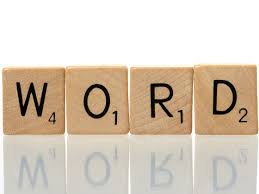
\includegraphics[scale=.3]{./Figures/word.jpeg}
% 	\caption{Imagen tomada de la página oficial del procesador\protect\footnotemark.}
% 	\label{fig:palabraIngles}
% \end{figure}

% \footnotetext{Imagen tomada de \url{https://goo.gl/images/i7C70w}}

% La figura y el epígrafe deben conformar una unidad cuyo significado principal pueda ser comprendido por el lector sin necesidad de leer el cuerpo central de la memoria. Para eso es necesario que el epígrafe sea todo lo detallado que corresponda y si en la figura se utilizan abreviaturas entonces aclarar su significado en el epígrafe o en la misma figura.



% \begin{figure}[ht]
% 	\centering
% 	
\includegraphics[scale=.37]{./Figures/questionMark.png}
% 	\caption{¿Por qué de pronto aparece esta figura?}
% 	\label{fig:questionMark}
% \end{figure}

% Nunca colocar una figura en el documento antes de hacer la primera referencia a ella, como se ilustra con la figura \cite{fig:questionMark}, porque sino el lector no comprenderá por qué de pronto aparece la figura en el documento, lo que distraerá su atención.

% Otra posibilidad es utilizar el entorno \textit{subfigure} para incluir más de una figura, como se puede ver en la figura \cite{fig:three graphs}. Notar que se pueden referenciar también las figuras internas individualmente de esta manera: \cite{fig:1de3}, \cite{fig:2de3} y \cite{fig:3de3}.
 
% \begin{figure}[!htpb]
%      \centering
%      \begin{subfigure}[b]{0.3\textwidth}
%          \centering
%          
\includegraphics[width=.65\textwidth]{./Figures/questionMark}
%          \caption{Un caption.}
%          \label{fig:1de3}
%      \end{subfigure}
%      \hfill
%      \begin{subfigure}[b]{0.3\textwidth}
%          \centering
%          
\includegraphics[width=.65\textwidth]{./Figures/questionMark}
%          \caption{Otro.}
%          \label{fig:2de3}
%      \end{subfigure}
%      \hfill
%      \begin{subfigure}[b]{0.3\textwidth}
%          \centering
%          
\includegraphics[width=.65\textwidth]{./Figures/questionMark}
%          \caption{Y otro más.}
%          \label{fig:3de3}
%      \end{subfigure}
%         \caption{Tres gráficos simples.}
%         \label{fig:three graphs}
% \end{figure}

% El código para generar las imágenes se encuentra disponible para su reutilización en el archivo \file{Chapter2.tex}.

% \subsection{Tablas}

% Para las tablas utilizar el mismo formato que para las figuras, sólo que el epígrafe se debe colocar arriba de la tabla, como se ilustra en la tabla \cite{tab:peces}. Observar que sólo algunas filas van con líneas visibles y notar el uso de las negritas para los encabezados.  La referencia se logra utilizando el comando \verb|\cite{<label>}| donde label debe estar definida dentro del entorno de la tabla.

% \begin{verbatim}
% \begin{table}[h]
% 	\centering
% 	\caption[caption corto]{caption largo más descriptivo}
% 	\begin{tabular}{l c c}    
% 		\toprule
% 		\textbf{Especie}     & \textbf{Tamaño} & \textbf{Valor}\\
% 		\midrule
% 		Amphiprion Ocellaris & 10 cm           & \$ 6.000 \\		
% 		Hepatus Blue Tang    & 15 cm           & \$ 7.000 \\
% 		Zebrasoma Xanthurus  & 12 cm           & \$ 6.800 \\
% 		\bottomrule
% 		\hline
% 	\end{tabular}
% 	\label{tab:peces}
% \end{table}
% \end{verbatim}


% \begin{table}[h]
% 	\centering
% 	\caption[caption corto]{caption largo más descriptivo.}
% 	\begin{tabular}{l c c}    
% 		\toprule
% 		\textbf{Especie} 	 & \textbf{Tamaño} 		& \textbf{Valor}  \\
% 		\midrule
% 		Amphiprion Ocellaris & 10 cm 				& \$ 6.000 \\		
% 		Hepatus Blue Tang	 & 15 cm				& \$ 7.000 \\
% 		Zebrasoma Xanthurus	 & 12 cm				& \$ 6.800 \\
% 		\bottomrule
% 		\hline
% 	\end{tabular}
% 	\label{tab:peces}
% \end{table}

% En cada capítulo se debe reiniciar el número de conteo de las figuras y las tablas, por ejemplo, figura 2.1 o tabla 2.1, pero no se debe reiniciar el conteo en cada sección. Por suerte la plantilla se encarga de esto por nosotros.

% \subsection{Ecuaciones}
% \label{sec:Ecuaciones}

% Al insertar ecuaciones en la memoria dentro de un entorno \textit{equation}, éstas se numeran en forma automática  y se pueden referir al igual que como se hace con las figuras y tablas, por ejemplo ver la ecuación \cite{eq:metric}.

% \begin{equation}
% 	\label{eq:metric}
% 	ds^2 = c^2 dt^2 \left( \frac{d\sigma^2}{1-k\sigma^2} + \sigma^2\left[ d\theta^2 + \sin^2\theta d\phi^2 \right] \right)
% \end{equation}
                                                        
% Es importante tener presente que si bien las ecuaciones pueden ser referidas por su número, también es correcto utilizar los dos puntos, como por ejemplo ``la expresión matemática que describe este comportamiento es la siguiente:''

% \begin{equation}
% 	\label{eq:schrodinger}
% 	\frac{\hbar^2}{2m}\nabla^2\Psi + V(\mathbf{r})\Psi = -i\hbar \frac{\partial\Psi}{\partial t}
% \end{equation}

% Para generar la ecuación \cite{eq:metric} se utilizó el siguiente código:

% \begin{verbatim}
% \begin{equation}
% 	\label{eq:metric}
% 	ds^2 = c^2 dt^2 \left( \frac{d\sigma^2}{1-k\sigma^2} + 
% 	\sigma^2\left[ d\theta^2 + 
% 	\sin^2\theta d\phi^2 \right] \right)
% \end{equation}
% \end{verbatim}

% Y para la ecuación \cite{eq:schrodinger}:

% \begin{verbatim}
% \begin{equation}
% 	\label{eq:schrodinger}
% 	\frac{\hbar^2}{2m}\nabla^2\Psi + V(\mathbf{r})\Psi = 
% 	-i\hbar \frac{\partial\Psi}{\partial t}
% \end{equation}

% \end{verbatim} 
% 	\chapter{Diseño e implementación} % Main chapter title

\label{Chapter3} % Change X to a consecutive number; for referencing this chapter elsewhere, use \ref{ChapterX}

Todos los capítulos deben comenzar con un breve párrafo introductorio que indique cuál es el contenido que se encontrará al leerlo.  La redacción sobre el contenido de la memoria debe hacerse en presente y todo lo referido al proyecto en pasado, siempre de modo impersonal.

\definecolor{mygreen}{rgb}{0,0.6,0}
\definecolor{mygray}{rgb}{0.5,0.5,0.5}
\definecolor{mymauve}{rgb}{0.58,0,0.82}

%%%%%%%%%%%%%%%%%%%%%%%%%%%%%%%%%%%%%%%%%%%%%%%%%%%%%%%%%%%%%%%%%%%%%%%%%%%%%
% parámetros para configurar el formato del código en los entornos lstlisting
%%%%%%%%%%%%%%%%%%%%%%%%%%%%%%%%%%%%%%%%%%%%%%%%%%%%%%%%%%%%%%%%%%%%%%%%%%%%%
\lstset{ %
  backgroundcolor=\color{white},   % choose the background color; you must add \usepackage{color} or \usepackage{xcolor}
  basicstyle=\footnotesize,        % the size of the fonts that are used for the code
  breakatwhitespace=false,         % sets if automatic breaks should only happen at whitespace
  breaklines=true,                 % sets automatic line breaking
  captionpos=b,                    % sets the caption-position to bottom
  commentstyle=\color{mygreen},    % comment style
  deletekeywords={...},            % if you want to delete keywords from the given language
  %escapeinside={\%*}{*)},          % if you want to add LaTeX within your code
  %extendedchars=true,              % lets you use non-ASCII characters; for 8-bits encodings only, does not work with UTF-8
  %frame=single,	                % adds a frame around the code
  keepspaces=true,                 % keeps spaces in text, useful for keeping indentation of code (possibly needs columns=flexible)
  keywordstyle=\color{blue},       % keyword style
  language=[ANSI]C,                % the language of the code
  %otherkeywords={*,...},           % if you want to add more keywords to the set
  numbers=left,                    % where to put the line-numbers; possible values are (none, left, right)
  numbersep=5pt,                   % how far the line-numbers are from the code
  numberstyle=\tiny\color{mygray}, % the style that is used for the line-numbers
  rulecolor=\color{black},         % if not set, the frame-color may be changed on line-breaks within not-black text (e.g. comments (green here))
  showspaces=false,                % show spaces everywhere adding particular underscores; it overrides 'showstringspaces'
  showstringspaces=false,          % underline spaces within strings only
  showtabs=false,                  % show tabs within strings adding particular underscores
  stepnumber=1,                    % the step between two line-numbers. If it's 1, each line will be numbered
  stringstyle=\color{mymauve},     % string literal style
  tabsize=2,	                   % sets default tabsize to 2 spaces
  title=\lstname,                  % show the filename of files included with \lstinputlisting; also try caption instead of title
  morecomment=[s]{/*}{*/}
}


%----------------------------------------------------------------------------------------
%	SECTION 1
%----------------------------------------------------------------------------------------
% \section{Análisis del software}
 
% La idea de esta sección es resaltar los problemas encontrados, los criterios utilizados y la justificación de las decisiones que se hayan tomado.

% Se puede agregar código o pseudocódigo dentro de un entorno lstlisting con el siguiente código:

% \begin{verbatim}
% \begin{lstlisting}[caption= "un epígrafe descriptivo"]
% 	las líneas de código irían aquí...
% \end{lstlisting}
% \end{verbatim}

% A modo de ejemplo:

% \begin{lstlisting}[label=cod:vControl,caption=Pseudocódigo del lazo principal de control.]  % Start your code-block

% #define MAX_SENSOR_NUMBER 3
% #define MAX_ALARM_NUMBER  6
% #define MAX_ACTUATOR_NUMBER 6

% uint32_t sensorValue[MAX_SENSOR_NUMBER];		
% FunctionalState alarmControl[MAX_ALARM_NUMBER];	//ENABLE or DISABLE
% state_t alarmState[MAX_ALARM_NUMBER];						//ON or OFF
% state_t actuatorState[MAX_ACTUATOR_NUMBER];			//ON or OFF

% void vControl() {

% 	initGlobalVariables();
	
% 	period = 500 ms;
		
% 	while(1) {

% 		ticks = xTaskGetTickCount();
		
% 		updateSensors();
		
% 		updateAlarms();
		
% 		controlActuators();
		
% 		vTaskDelayUntil(&ticks, period);
% 	}
% }
% \end{lstlisting}




% 	% Chapter Template

\chapter{Ensayos y resultados} % Main chapter title

\label{Chapter4} % Change X to a consecutive number; for referencing this chapter elsewhere, use \ref{ChapterX}
Todos los capítulos deben comenzar con un breve párrafo introductorio que indique cuál es el contenido que se encontrará al leerlo.  La redacción sobre el contenido de la memoria debe hacerse en presente y todo lo referido al proyecto en pasado, siempre de modo impersonal.

%----------------------------------------------------------------------------------------
%	SECTION 1
%----------------------------------------------------------------------------------------

% \section{Pruebas funcionales del hardware}
% \label{sec:pruebasHW}

% La idea de esta sección es explicar cómo se hicieron los ensayos, qué resultados se obtuvieron y analizarlos.
 
% 	% Chapter Template

\chapter{Conclusiones} % Main chapter title

\label{Chapter5} % Change X to a consecutive number; for referencing this chapter elsewhere, use \ref{ChapterX}
Todos los capítulos deben comenzar con un breve párrafo introductorio que indique cuál es el contenido que se encontrará al leerlo.  La redacción sobre el contenido de la memoria debe hacerse en presente y todo lo referido al proyecto en pasado, siempre de modo impersonal.


%----------------------------------------------------------------------------------------

%----------------------------------------------------------------------------------------
%	SECTION 1
%----------------------------------------------------------------------------------------

% \section{Conclusiones generales }

% La idea de esta sección es resaltar cuáles son los principales aportes del trabajo realizado y cómo se podría continuar. Debe ser especialmente breve y concisa. Es buena idea usar un listado para enumerar los logros obtenidos.

% En esta sección no se deben incluir ni tablas ni gráficos.

% Algunas preguntas que pueden servir para completar este capítulo:

% \begin{itemize}
% \item ¿Cuál es el grado de cumplimiento de los requerimientos?
% \item ¿Cuán fielmente se puedo seguir la planificación original (cronograma incluido)?
% \item ¿Se manifestó algunos de los riesgos identificados en la planificación? ¿Fue efectivo el plan de mitigación? ¿Se debió aplicar alguna otra acción no contemplada previamente?
% \item Si se debieron hacer modificaciones a lo planificado ¿Cuáles fueron las causas y los efectos?
% \item ¿Qué técnicas resultaron útiles para el desarrollo del proyecto y cuáles no tanto?
% \end{itemize}


% %----------------------------------------------------------------------------------------
% %	SECTION 2
% %----------------------------------------------------------------------------------------
% \section{Próximos pasos}

% Acá se indica cómo se podría continuar el trabajo más adelante.
 
% \end{verbatim}

% Los apéndices también deben escribirse en archivos .tex separados, que se deben ubicar dentro de la carpeta \emph{Appendices}. Los apéndices vienen comentados por defecto con el caracter \code{\%} y para incluirlos simplemente se debe eliminar dicho caracter.

% Finalmente, se encuentra el código para incluir la bibliografía en el documento final.  Este código tampoco debe modificarse. La metodología para trabajar las referencias bibliográficas se desarrolla en la sección \ref{sec:biblio}.
% %----------------------------------------------------------------------------------------

% \section{Bibliografía}
% \label{sec:biblio}

% Las opciones de formato de la bibliografía se controlan a través del paquete de latex \option{biblatex} que se incluye en la memoria en el archivo memoria.tex.  Estas opciones determinan cómo se generan las citas bibliográficas en el cuerpo del documento y cómo se genera la bibliografía al final de la memoria.

% En el preámbulo se puede encontrar el código que incluye el paquete biblatex, que no requiere ninguna modificación del usuario de la plantilla, y que contiene las siguientes opciones:

% \begin{lstlisting}
% \usepackage[backend=bibtex,
% 	natbib=true, 
% 	style=numeric, 
% 	sorting=none]
% {biblatex}
% \end{lstlisting}

% En el archivo \file{reference.bib} se encuentran las referencias bibliográficas que se pueden citar en el documento.  Para incorporar una nueva cita al documento lo primero es agregarla en este archivo con todos los campos necesario.  Todas las entradas bibliográficas comienzan con $@$ y una palabra que define el formato de la entrada.  Para cada formato existen campos obligatorios que deben completarse. No importa el orden en que las entradas estén definidas en el archivo .bib.  Tampoco es importante el orden en que estén definidos los campos de una entrada bibliográfica. A continuación se muestran algunos ejemplos:

% \begin{lstlisting}
% @ARTICLE{ARTICLE:1,
%     AUTHOR="John Doe",
%     TITLE="Title",
%     JOURNAL="Journal",
%     YEAR="2017",
% }
% \end{lstlisting}


% \begin{lstlisting}
% @BOOK{BOOK:1,
%     AUTHOR="John Doe",
%     TITLE="The Book without Title",
%     PUBLISHER="Dummy Publisher",
%     YEAR="2100",
% }
% \end{lstlisting}


% \begin{lstlisting}
% @INBOOK{BOOK:2,
%     AUTHOR="John Doe",
%     TITLE="The Book without Title",
%     PUBLISHER="Dummy Publisher",
%     YEAR="2100",
%     PAGES="100-200",
% }
% \end{lstlisting}


% \begin{lstlisting}
% @MISC{WEBSITE:1,
%     HOWPUBLISHED = "\url{http://example.com}",
%     AUTHOR = "Intel",
%     TITLE = "Example Website",
%     MONTH = "12",
%     YEAR = "1988",
%     URLDATE = {2012-11-26}
% }
% \end{lstlisting}

% Se debe notar que los nombres \emph{ARTICLE:1}, \emph{BOOK:1}, \emph{BOOK:2} y \emph{WEBSITE:1} son nombres de fantasía que le sirve al autor del documento para identificar la entrada. En este sentido, se podrían reemplazar por cualquier otro nombre.  Tampoco es necesario poner : seguido de un número, en los ejemplos sólo se incluye como un posible estilo para identificar las entradas.

% La entradas se citan en el documento con el comando: 

% \begin{verbatim}
% \citep{nombre_de_la_entrada}
% \end{verbatim}

% Y cuando se usan, se muestran así: \citep{ARTICLE:1}, \citep{BOOK:1}, \citep{BOOK:2}, \citep{WEBSITE:1}.  Notar cómo se conforma la sección Bibliografía al final del documento.

% Finalmente y como se mencionó en la subsección \ref{subsec:configurando}, para actualizar las referencias bibliográficas tanto en la sección bibliografía como las citas en el cuerpo del documento, se deben ejecutar las herramientas de compilación PDFLaTeX, BibTeX, PDFLaTeX, PDFLaTeX, en ese orden.  Este procedimiento debería resolver cualquier mensaje "Citation xxxxx on page x undefined".

\chapter{Introducción específica} 

\label{Chapter2}

Este capítulo presenta los conceptos y componentes centrales que sustentan el trabajo. Se introducen los sistemas de recomendación y sus enfoques principales, se describen las fuentes de información empleadas y se detallan las plataformas y herramientas utilizadas para el procesamiento de datos, el modelado y la gestión de experimentos, que conforman la base tecnológica de la solución propuesta.
%----------------------------------------------------------------------------------------

\section{Sistemas de recomendación}

Los sistemas de recomendación constituyen una de las aplicaciones más extendidas de la inteligencia artificial \cite{BOOK:Ricci2015,ARTICLE:Adomavicius2005}, con un papel central en la reducción de la sobrecarga de información y en la optimización de decisiones de consumo. Su finalidad es generar sugerencias personalizadas que se ajusten a las características de cada cliente, lo que incrementa la relevancia de los productos ofrecidos y mejora la experiencia general de interacción con la empresa.

\subsection{Funcionamiento de los sistemas de recomendación}

El eje central del enfoque consiste en identificar relaciones de similitud entre productos, clientes o interacciones \cite{BOOK:Ricci2015}. Estas relaciones pueden establecerse desde diferentes perspectivas. En primer lugar, es posible medir la similitud entre productos, lo que permite agrupar aquellos que suelen adquirirse en conjunto o que comparten atributos comunes. En segundo lugar, puede analizarse la similitud entre clientes, de modo que las preferencias observadas en un grupo con comportamientos semejantes permitan anticipar las elecciones de otros con perfiles cercanos. Por último, también resulta clave la similitud entre interacciones, que considera el historial de comportamientos de un cliente, como sus compras o búsquedas, para anticipar futuras decisiones.

Un ejemplo ilustrativo, representado en la figura \ref{fig:ejemploSimilitud}, puede plantearse en la industria de bebidas. Supongamos que cada marca de cerveza se representa como un vector en un espacio definido por atributos, como \texttt{tradicional versus innovador} y \texttt{masivo versus \textit{premium}}. En ese espacio, una lager clásica de gran consumo quedaría ubicada cerca de otras variedades tradicionales y de alcance masivo, mientras que una IPA artesanal o una edición limitada se situarían en la región asociada a lo \textit{premium} e innovador. El sistema de recomendación aprovecha esta representación para calcular distancias o similaridades entre productos. Si un cliente suele elegir artículos situados en torno al cuadrante de \texttt{\textit{premium}–tradicional}, el modelo infiere que probablemente muestre interés por otras marcas que ocupan posiciones cercanas en ese mismo espacio vectorial. De esta manera, la proximidad entre vectores se convierte en un indicador de afinidad, que guía la generación de recomendaciones personalizadas.

\begin{figure}[htpb]
	\centering
	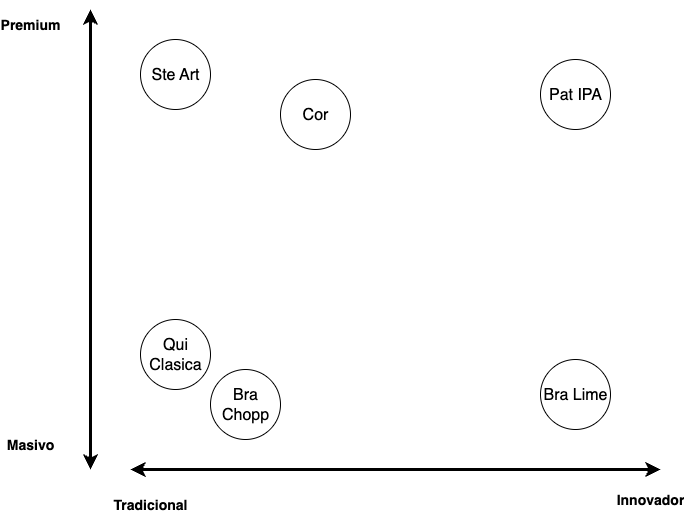
\includegraphics[scale=.4]{./Figures/ejemploSimilitud.png}
	\caption{Ejemplo de representación de marcas de cerveza en un espacio de atributos.}
	\label{fig:ejemploSimilitud}
\end{figure}

\subsection{Tipos de \textit{feedback}}

El tipo de información disponible para alimentar un sistema de recomendación también es determinante. Se distinguen dos formas principales de retroalimentación \cite{ARTICLE:Hu2008}. La retroalimentación explícita consiste en la valoración directa que realizan los clientes sobre los productos, como calificaciones numéricas, encuestas o reseñas. La retroalimentación implícita, en cambio, se infiere del comportamiento de los clientes, ya sea a través de sus compras, búsquedas o interacciones digitales. En el ámbito B2B, donde no es común que los clientes asignen calificaciones explícitas, predominan las señales implícitas, lo que plantea desafíos adicionales para la construcción de modelos precisos.

\subsection{Filtrado colaborativo}

El filtrado colaborativo se apoya en la hipótesis de que usuarios similares tienden a preferir ítems similares, lo que puede abordarse mediante enfoques \textit{user-based} o \textit{item-based} \cite{ARTICLE:Sarwar2001}. Su implementación moderna se basa en factorización matricial \cite{ARTICLE:Koren2009}.

En la modalidad \textit{user-based}, se recomienda a un cliente productos que fueron consumidos por otros con patrones de compra semejantes. En la modalidad \textit{item-based}, se priorizan productos que suelen aparecer en conjunto en los historiales de distintos clientes. 

El filtrado colaborativo suele implementarse mediante técnicas de factorización matricial. Dado un conjunto de $m$ usuarios y $n$ productos, se construye una matriz de interacciones $R \in \mathbb{R}^{m \times n}$, donde cada celda refleja el vínculo entre un cliente y un producto. El objetivo consiste en aproximar esta matriz como el producto de dos matrices de menor dimensión, como se puede observar en \ref{eq:factorizacion}.

\begin{equation}
\label{eq:factorizacion}
R \approx U \cdot V^T
\end{equation}

donde $U \in \mathbb{R}^{m \times k}$ representa a los usuarios en un espacio latente de dimensión $k$, y $V \in \mathbb{R}^{n \times k}$ representa a los ítems en ese mismo espacio. La predicción de la afinidad del usuario $i$ con el ítem $j$ se calcula en \ref{eq:prediccion_cf} como el producto escalar entre los vectores latentes correspondientes.

\begin{equation}
\label{eq:prediccion_cf}
\hat{r}_{ij} = u_i \cdot v_j^T
\end{equation}

Este modelo permite capturar relaciones complejas entre clientes y productos a partir de información implícita, aunque presenta limitaciones frente al problema del arranque en frío, cuando no existe historial suficiente de interacciones.

\subsection{Sistemas basados en contenido}

Otro enfoque ampliamente utilizado es el de los sistemas basados en contenido, que centran la recomendación en las características de los productos y en el perfil de cada cliente \cite{ARTICLE:Pazzani2007}. En este caso, se representa a cada producto por un vector de atributos y se construye un perfil para cada cliente que refleja la importancia relativa de esos atributos en función de sus elecciones pasadas. La predicción de relevancia para recomendar un producto $j$ a un cliente $i$ puede expresarse de manera simplificada como en \ref{eq:prediccion_cb}.

\begin{equation}
\label{eq:prediccion_cb}
\hat{r}_{ij} = w_i \cdot x_j
\end{equation}

donde $x_j$ es el vector de atributos del producto y $w_i$ representa el perfil del cliente. Este método permite recomendar productos nuevos o poco frecuentes siempre que exista información suficiente sobre sus atributos, lo que lo convierte en un complemento natural del filtrado colaborativo.

%----------------------------------------------------------------------------------------

\section{Fuentes de información}


%  -- Muy especifico sobre el trabajo, lo dejo para el cap 3 --
% El desarrollo del sistema de recomendación se apoya en un conjunto diverso de datos que, en su integración, permiten construir una representación enriquecida de la relación cliente–producto. Estas fuentes incluyen información transaccional, eventos de interacción en la aplicación BEES y atributos contextuales de clientes y productos. En conjunto, estos elementos aportan evidencia implícita de interés y afinidad, y constituyen la base para la estimación de scores personalizados.

% Los datos transaccionales reflejan las compras efectivamente realizadas por cada cliente. Dentro de esta categoría se consideran las siguientes variables: volumen adquirido por producto, frecuencia de compra, recencia de la última operación, monetización total y participación relativa de cada producto en el mix de compras del cliente. Estas medidas permiten capturar el grado de preferencia y relevancia actual de cada artículo en la cartera de cada punto de venta.

% A su vez, se incorporan eventos de comportamiento generados en la aplicación BEES, los cuales funcionan como señales implícitas de interés. Entre ellos se incluyen agregados y remociones de productos del carrito, visualizaciones de fichas de producto, búsquedas realizadas, calificaciones o reseñas, y clics en promociones. Estos registros aportan información complementaria sobre el proceso de consideración del cliente, incluso en los casos en los que no se concreta una transacción.

% La caracterización se completa con variables de contexto asociadas tanto a clientes como a productos. Del lado del cliente, se integran atributos como el canal comercial y la ubicación geográfica. Del lado del producto, se consideran propiedades como marca, segmento, calibre y participación de mercado. Este conjunto de información contextual permite capturar heterogeneidades relevantes que condicionan la relación de afinidad.

% De esta forma, la combinación de datos transaccionales, eventos digitales y atributos contextuales permite construir una representación integral de las interacciones cliente–producto, sobre la cual se sustenta el modelado de afinidad.

El funcionamiento de los sistemas de recomendación se apoya en diversas fuentes de información \cite{BOOK:Ricci2015,ARTICLE:Adomavicius2005} que, al combinarse, permiten construir una representación más completa de la relación entre usuarios y productos. Estas fuentes pueden clasificarse en tres grandes categorías: datos transaccionales, señales de interacción y atributos contextuales.

Los datos transaccionales reflejan las operaciones efectivamente realizadas, como compras, alquileres o reproducciones. Constituyen una evidencia directa de preferencia, ya que expresan decisiones concretas de los usuarios respecto a determinados productos o servicios.

Las señales de interacción incluyen registros de comportamiento que no necesariamente culminan en una transacción, pero que aportan información implícita de interés. Las señales implícitas, como visualizaciones o clics, resultan especialmente valiosas en contextos digitales \cite{ARTICLE:Hu2008,ARTICLE:Covington2016}. Ejemplos de este tipo de datos son las visualizaciones de fichas de producto, las búsquedas realizadas en una plataforma, las adiciones y eliminaciones en un carrito digital o las calificaciones otorgadas. Estas interacciones permiten identificar patrones de consideración más allá de la compra final.

Finalmente, los atributos contextuales corresponden a características adicionales tanto de los usuarios como de los productos. Del lado de los usuarios, se pueden incluir variables demográficas, geográficas o vinculadas al canal de consumo. Del lado de los productos, se consideran atributos como categoría, marca, segmento o características técnicas. Este conjunto de información enriquece la representación de afinidad, al capturar heterogeneidades que condicionan las recomendaciones.

De esta forma, la integración de datos transaccionales, señales de interacción y atributos contextuales constituye la base informativa sobre la cual se construyen los diferentes enfoques de recomendación. La disponibilidad y calidad de estas fuentes son determinantes para el desempeño de los modelos y para la capacidad de generar sugerencias precisas y relevantes.


%----------------------------------------------------------------------------------------

\section{Herramientas utilizadas}

%  -- Muy especifico sobre el trabajo, lo dejo para el cap 3 --
% El desarrollo del trabajo se apoyó en un conjunto de herramientas tecnológicas que permitieron gestionar de manera eficiente el ciclo de vida completo del sistema de recomendación, desde la preparación de datos hasta el despliegue de modelos.

% En primer lugar, se utilizó la plataforma Databricks, que combina capacidades de procesamiento distribuido con un entorno colaborativo para el análisis de datos. Databricks permitió integrar múltiples fuentes, realizar transformaciones a gran escala con \texttt{PySpark} y organizar flujos de trabajo de forma reproducible y escalable. Su uso facilitó tanto la exploración inicial como la construcción de pipelines de ingeniería de atributos.A

% En segundo lugar, se empleó \texttt{MLflow} como herramienta de gestión del ciclo de vida de modelos. A través de esta plataforma se registraron experimentos, parámetros, métricas y versiones de modelos, lo que aseguró trazabilidad y comparabilidad entre distintos enfoques. Asimismo, se utilizaron las funcionalidades de almacenamiento y versionado de artefactos para garantizar la reproducibilidad de resultados y la posibilidad de mantener un repositorio consolidado de modelos entrenados.

% El trabajo también se apoyó en bibliotecas de aprendizaje automático ampliamente utilizadas en la comunidad científica y profesional. Entre ellas se destaca \texttt{MLlib}, utilizada para implementar la factorización matricial con \texttt{ALS}. Asimismo, se empleó \texttt{LightFM} para el desarrollo de modelos híbridos de filtrado colaborativo. Finalmente, se incorporó \texttt{PyTorch} como entorno de \textit{deep learning}, lo que permitió construir arquitecturas más complejas capaces de capturar patrones no lineales en las interacciones cliente–producto. Adicionalmente, se utilizaron bibliotecas de visualización como \texttt{matplotlib} y \texttt{seaborn} para generar representaciones gráficas que complementaron el análisis exploratorio y la evaluación de resultados.

% Finalmente, se recurrió a entornos de control de versiones y colaboración, en particular \texttt{GitHub}, lo que permitió organizar el código en repositorios estructurados, registrar cambios de manera sistemática y facilitar la integración de componentes en distintas fases del trabajo.

% En conjunto, estas herramientas proporcionaron una infraestructura sólida para desarrollar, evaluar y documentar el sistema de recomendación, lo que aseguró tanto la calidad técnica como la escalabilidad del enfoque implementado.

% --- MUY GENERICO ---

% El desarrollo de sistemas de recomendación requiere una infraestructura tecnológica que permita gestionar de manera eficiente el ciclo de vida completo de los modelos, desde la preparación de datos hasta su despliegue en entornos productivos. Para ello, se emplean plataformas y herramientas que integran capacidades de procesamiento, experimentación y gestión colaborativa.

% En primer lugar, las plataformas de procesamiento distribuido resultan fundamentales para manipular grandes volúmenes de datos y realizar transformaciones a escala. Estas soluciones suelen combinar entornos colaborativos con motores de cálculo paralelizado, lo que facilita tanto la exploración inicial como la construcción de flujos de trabajo reproducibles.

% En segundo lugar, los sistemas de gestión del ciclo de vida de modelos (MLOps) permiten registrar experimentos, parámetros, métricas y versiones de modelos. Estas herramientas aseguran trazabilidad, reproducibilidad y comparabilidad entre diferentes enfoques, además de posibilitar el almacenamiento y versionado de artefactos.

% Adicionalmente, se utilizan bibliotecas de aprendizaje automático y profundo que constituyen estándares en la comunidad científica y profesional. Entre ellas se destacan entornos para la implementación de algoritmos clásicos de recomendación, bibliotecas para modelos híbridos y marcos de trabajo de deep learning que permiten capturar patrones complejos en las interacciones entre clientes y productos. Estas soluciones suelen complementarse con bibliotecas de visualización orientadas a generar representaciones gráficas que apoyen el análisis exploratorio y la evaluación de resultados.

% Finalmente, las plataformas de control de versiones y colaboración cumplen un rol central en la organización del código, el registro de cambios y la integración de componentes en distintas fases del desarrollo. Estas herramientas permiten estructurar repositorios, asegurar calidad en los procesos de desarrollo y facilitar la coordinación entre equipos.

% En conjunto, este ecosistema de plataformas y bibliotecas constituye la base tecnológica sobre la cual se implementan los sistemas de recomendación modernos, garantizando tanto la calidad técnica como la escalabilidad de las soluciones.

El desarrollo de este trabajo se apoyó en un conjunto de herramientas tecnológicas que facilitaron la gestión integral del ciclo de vida del sistema de recomendación. A continuación, se detallan las principales plataformas, bibliotecas y entornos empleados, junto con su función específica en el proceso.

\subsection{Plataformas de procesamiento distribuido}

El procesamiento y consolidación de grandes volúmenes de información se llevó a cabo en la plataforma Databricks \cite{ARTICLE:Databricks}, que integra un entorno colaborativo con un motor de cómputo distribuido basado en Apache Spark \cite{ARTICLE:Spark2012}. Esta herramienta permitió orquestar la ingestión de datos, ejecutar transformaciones a gran escala mediante PySpark y garantizar reproducibilidad en los flujos de trabajo. El uso de Databricks resultó fundamental para integrar múltiples fuentes y preparar los insumos que alimentaron las etapas de análisis y modelado.

\subsection{Gestión del ciclo de vida de modelos}

Para la gestión del ciclo de vida de los modelos se empleó MLflow \cite{ARTICLE:MLflow2018}, plataforma que facilita el registro de experimentos, parámetros, métricas y versiones de modelos. Esta herramienta permitió mantener trazabilidad entre las distintas ejecuciones, asegurar comparabilidad de resultados y almacenar los artefactos generados (modelos entrenados y estructuras derivadas). De este modo, se consolidó un repositorio ordenado que garantizó reproducibilidad y control en la experimentación.

\subsection{Bibliotecas de aprendizaje automático y profundo}

En el desarrollo de los modelos se emplearon distintas bibliotecas que constituyen estándares en la comunidad científica y profesional. Se utilizó MLlib para implementar el filtrado colaborativo mediante factorización matricial con el algoritmo Alternating Least Squares (ALS) \cite{ARTICLE:ALS2008}, mientras que LightFM \cite{ARTICLE:LightFM2015} permitió construir un modelo híbrido que combina señales de interacción implícita con atributos de clientes y productos. Adicionalmente, se recurrió a PyTorch como entorno de deep learning para el diseño de arquitecturas neuronales capaces de capturar relaciones no lineales y complejas en los datos. 

\subsection{Bibliotecas de visualización}

Para el análisis visual y la generación de gráficos se utilizaron bibliotecas como Matplotlib \cite{ARTICLE:Matplotlib2007} y Seaborn \cite{ARTICLE:Seaborn2021}, que facilitaron la representación gráfica tanto de la información explorada como de los resultados obtenidos en las distintas fases del trabajo.

\subsection{Control de versiones y colaboración}

La organización y versionado del código se gestionaron mediante GitHub \cite{ARTICLE:GitHub}, que permitió estructurar los repositorios, registrar cambios de manera sistemática y facilitar la colaboración. El uso de esta plataforma aseguró orden en el desarrollo, trazabilidad de modificaciones y una integración eficiente de los distintos componentes del sistema.

\subsection{Consideraciones finales}

En conjunto, estas herramientas brindaron una infraestructura robusta para abordar todas las etapas del desarrollo del sistema de recomendación, desde la preparación de los datos hasta la evaluación y almacenamiento de modelos. Cabe destacar que la calidad de una implementación no depende únicamente del algoritmo utilizado, sino también de la solidez del entorno técnico que la respalda. El uso articulado de estas herramientas permitió asegurar la reproducibilidad de los resultados, la eficiencia en el manejo de datos, la trazabilidad de las decisiones y la escalabilidad del sistema desarrollado. En el contexto de una solución real, contar con esta base técnica resulta clave para garantizar tanto la calidad técnica como la posibilidad de evolución futura del sistema.

%----------------------------------------------------------------------------------------


% \section{Estilo y convenciones}
% \label{sec:ejemplo}

% \subsection{Uso de mayúscula inicial para los título de secciones}

% Si en el texto se hace alusión a diferentes partes del trabajo referirse a ellas como capítulo, sección o subsección según corresponda. Por ejemplo: ``En el capítulo \cite{Chapter1} se explica tal cosa'', o ``En la sección \cite{sec:ejemplo} se presenta lo que sea'', o ``En la subsección \cite{subsec:ejemplo} se discute otra cosa''.

% Cuando se quiere poner una lista tabulada, se hace así:

% \begin{itemize}
% 	\item Este es el primer elemento de la lista.
% 	\item Este es el segundo elemento de la lista.
% \end{itemize}

% Notar el uso de las mayúsculas y el punto al final de cada elemento.

% Si se desea poner una lista numerada el formato es este:

% \begin{enumerate}
% 	\item Este es el primer elemento de la lista.
% 	\item Este es el segundo elemento de la lista.
% \end{enumerate}

% Notar el uso de las mayúsculas y el punto al final de cada elemento.

% \subsection{Este es el título de una subsección}
% \label{subsec:ejemplo}

% Se recomienda no utilizar \textbf{texto en negritas} en ningún párrafo, ni tampoco texto \underline{subrayado}. En cambio sí se debe utilizar \textit{texto en itálicas} para palabras en un idioma extranjero, al menos la primera vez que aparecen en el texto. En el caso de palabras que estamos inventando se deben utilizar ``comillas'', así como también para citas textuales. Por ejemplo, un \textit{digital filter} es una especie de ``selector'' que permite separar ciertos componentes armónicos en particular.

% La escritura debe ser impersonal. Por ejemplo, no utilizar ``el diseño del firmware lo hice de acuerdo con tal principio'', sino ``el firmware fue diseñado utilizando tal principio''. 

% El trabajo es algo que al momento de escribir la memoria se supone que ya está concluido, entonces todo lo que se refiera a hacer el trabajo se narra en tiempo pasado, porque es algo que ya ocurrió. Por ejemplo, "se diseñó el firmware empleando la técnica de test driven development".

% En cambio, la memoria es algo que está vivo cada vez que el lector la lee. Por eso transcurre siempre en tiempo presente, como por ejemplo:

% ``En el presente capítulo se da una visión global sobre las distintas pruebas realizadas y los resultados obtenidos. Se explica el modo en que fueron llevados a cabo los test unitarios y las pruebas del sistema''.

% Se recomienda no utilizar una sección de glosario sino colocar la descripción de las abreviaturas como parte del mismo cuerpo del texto. Por ejemplo, RTOS (\textit{Real Time Operating System}, Sistema Operativo de Tiempo Real) o en caso de considerarlo apropiado mediante notas a pie de página.

% Si se desea indicar alguna página web utilizar el siguiente formato de referencias bibliográficas, dónde las referencias se detallan en la sección de bibliografía de la memoria, utilizado el formato establecido por IEEE en \citep{IEEE:citation}. Por ejemplo, ``el presente trabajo se basa en la plataforma EDU-CIAA-NXP \citep{CIAA}, la cual...''.

% \subsection{Figuras} 

% Al insertar figuras en la memoria se deben considerar determinadas pautas. Para empezar, usar siempre tipografía claramente legible. Luego, tener claro que \textbf{es incorrecto} escribir por ejemplo esto: ``El diseño elegido es un cuadrado, como se ve en la siguiente figura:''

% \begin{figure}[h]
% \centering
% 
\includegraphics[scale=.45]{./Figures/cuadradoAzul.png}
% \end{figure}

% La forma correcta de utilizar una figura es con referencias cruzadas, por ejemplo: ``Se eligió utilizar un cuadrado azul para el logo, como puede observarse en la figura \cite{fig:cuadradoAzul}''.

% \begin{figure}[ht]
% 	\centering
% 	
\includegraphics[scale=.45]{./Figures/cuadradoAzul.png}
% 	\caption{Ilustración del cuadrado azul que se eligió para el diseño del logo.}
% 	\label{fig:cuadradoAzul}
% \end{figure}

% El texto de las figuras debe estar siempre en español, excepto que se decida reproducir una figura original tomada de alguna referencia. En ese caso la referencia de la cual se tomó la figura debe ser indicada en el epígrafe de la figura e incluida como una nota al pie, como se ilustra en la figura \cite{fig:palabraIngles}.

% \begin{figure}[htpb]
% 	\centering
% 	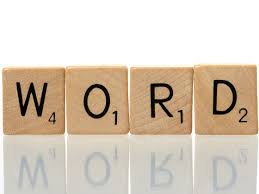
\includegraphics[scale=.3]{./Figures/word.jpeg}
% 	\caption{Imagen tomada de la página oficial del procesador\protect\footnotemark.}
% 	\label{fig:palabraIngles}
% \end{figure}

% \footnotetext{Imagen tomada de \url{https://goo.gl/images/i7C70w}}

% La figura y el epígrafe deben conformar una unidad cuyo significado principal pueda ser comprendido por el lector sin necesidad de leer el cuerpo central de la memoria. Para eso es necesario que el epígrafe sea todo lo detallado que corresponda y si en la figura se utilizan abreviaturas entonces aclarar su significado en el epígrafe o en la misma figura.



% \begin{figure}[ht]
% 	\centering
% 	
\includegraphics[scale=.37]{./Figures/questionMark.png}
% 	\caption{¿Por qué de pronto aparece esta figura?}
% 	\label{fig:questionMark}
% \end{figure}

% Nunca colocar una figura en el documento antes de hacer la primera referencia a ella, como se ilustra con la figura \cite{fig:questionMark}, porque sino el lector no comprenderá por qué de pronto aparece la figura en el documento, lo que distraerá su atención.

% Otra posibilidad es utilizar el entorno \textit{subfigure} para incluir más de una figura, como se puede ver en la figura \cite{fig:three graphs}. Notar que se pueden referenciar también las figuras internas individualmente de esta manera: \cite{fig:1de3}, \cite{fig:2de3} y \cite{fig:3de3}.
 
% \begin{figure}[!htpb]
%      \centering
%      \begin{subfigure}[b]{0.3\textwidth}
%          \centering
%          
\includegraphics[width=.65\textwidth]{./Figures/questionMark}
%          \caption{Un caption.}
%          \label{fig:1de3}
%      \end{subfigure}
%      \hfill
%      \begin{subfigure}[b]{0.3\textwidth}
%          \centering
%          
\includegraphics[width=.65\textwidth]{./Figures/questionMark}
%          \caption{Otro.}
%          \label{fig:2de3}
%      \end{subfigure}
%      \hfill
%      \begin{subfigure}[b]{0.3\textwidth}
%          \centering
%          
\includegraphics[width=.65\textwidth]{./Figures/questionMark}
%          \caption{Y otro más.}
%          \label{fig:3de3}
%      \end{subfigure}
%         \caption{Tres gráficos simples.}
%         \label{fig:three graphs}
% \end{figure}

% El código para generar las imágenes se encuentra disponible para su reutilización en el archivo \file{Chapter2.tex}.

% \subsection{Tablas}

% Para las tablas utilizar el mismo formato que para las figuras, sólo que el epígrafe se debe colocar arriba de la tabla, como se ilustra en la tabla \cite{tab:peces}. Observar que sólo algunas filas van con líneas visibles y notar el uso de las negritas para los encabezados.  La referencia se logra utilizando el comando \verb|\cite{<label>}| donde label debe estar definida dentro del entorno de la tabla.

% \begin{verbatim}
% \begin{table}[h]
% 	\centering
% 	\caption[caption corto]{caption largo más descriptivo}
% 	\begin{tabular}{l c c}    
% 		\toprule
% 		\textbf{Especie}     & \textbf{Tamaño} & \textbf{Valor}\\
% 		\midrule
% 		Amphiprion Ocellaris & 10 cm           & \$ 6.000 \\		
% 		Hepatus Blue Tang    & 15 cm           & \$ 7.000 \\
% 		Zebrasoma Xanthurus  & 12 cm           & \$ 6.800 \\
% 		\bottomrule
% 		\hline
% 	\end{tabular}
% 	\label{tab:peces}
% \end{table}
% \end{verbatim}


% \begin{table}[h]
% 	\centering
% 	\caption[caption corto]{caption largo más descriptivo.}
% 	\begin{tabular}{l c c}    
% 		\toprule
% 		\textbf{Especie} 	 & \textbf{Tamaño} 		& \textbf{Valor}  \\
% 		\midrule
% 		Amphiprion Ocellaris & 10 cm 				& \$ 6.000 \\		
% 		Hepatus Blue Tang	 & 15 cm				& \$ 7.000 \\
% 		Zebrasoma Xanthurus	 & 12 cm				& \$ 6.800 \\
% 		\bottomrule
% 		\hline
% 	\end{tabular}
% 	\label{tab:peces}
% \end{table}

% En cada capítulo se debe reiniciar el número de conteo de las figuras y las tablas, por ejemplo, figura 2.1 o tabla 2.1, pero no se debe reiniciar el conteo en cada sección. Por suerte la plantilla se encarga de esto por nosotros.

% \subsection{Ecuaciones}
% \label{sec:Ecuaciones}

% Al insertar ecuaciones en la memoria dentro de un entorno \textit{equation}, éstas se numeran en forma automática  y se pueden referir al igual que como se hace con las figuras y tablas, por ejemplo ver la ecuación \cite{eq:metric}.

% \begin{equation}
% 	\label{eq:metric}
% 	ds^2 = c^2 dt^2 \left( \frac{d\sigma^2}{1-k\sigma^2} + \sigma^2\left[ d\theta^2 + \sin^2\theta d\phi^2 \right] \right)
% \end{equation}
                                                        
% Es importante tener presente que si bien las ecuaciones pueden ser referidas por su número, también es correcto utilizar los dos puntos, como por ejemplo ``la expresión matemática que describe este comportamiento es la siguiente:''

% \begin{equation}
% 	\label{eq:schrodinger}
% 	\frac{\hbar^2}{2m}\nabla^2\Psi + V(\mathbf{r})\Psi = -i\hbar \frac{\partial\Psi}{\partial t}
% \end{equation}

% Para generar la ecuación \cite{eq:metric} se utilizó el siguiente código:

% \begin{verbatim}
% \begin{equation}
% 	\label{eq:metric}
% 	ds^2 = c^2 dt^2 \left( \frac{d\sigma^2}{1-k\sigma^2} + 
% 	\sigma^2\left[ d\theta^2 + 
% 	\sin^2\theta d\phi^2 \right] \right)
% \end{equation}
% \end{verbatim}

% Y para la ecuación \cite{eq:schrodinger}:

% \begin{verbatim}
% \begin{equation}
% 	\label{eq:schrodinger}
% 	\frac{\hbar^2}{2m}\nabla^2\Psi + V(\mathbf{r})\Psi = 
% 	-i\hbar \frac{\partial\Psi}{\partial t}
% \end{equation}

% \end{verbatim}
\chapter{Diseño e implementación} % Main chapter title

\label{Chapter3} % Change X to a consecutive number; for referencing this chapter elsewhere, use \ref{ChapterX}

Todos los capítulos deben comenzar con un breve párrafo introductorio que indique cuál es el contenido que se encontrará al leerlo.  La redacción sobre el contenido de la memoria debe hacerse en presente y todo lo referido al proyecto en pasado, siempre de modo impersonal.

\definecolor{mygreen}{rgb}{0,0.6,0}
\definecolor{mygray}{rgb}{0.5,0.5,0.5}
\definecolor{mymauve}{rgb}{0.58,0,0.82}

%%%%%%%%%%%%%%%%%%%%%%%%%%%%%%%%%%%%%%%%%%%%%%%%%%%%%%%%%%%%%%%%%%%%%%%%%%%%%
% parámetros para configurar el formato del código en los entornos lstlisting
%%%%%%%%%%%%%%%%%%%%%%%%%%%%%%%%%%%%%%%%%%%%%%%%%%%%%%%%%%%%%%%%%%%%%%%%%%%%%
\lstset{ %
  backgroundcolor=\color{white},   % choose the background color; you must add \usepackage{color} or \usepackage{xcolor}
  basicstyle=\footnotesize,        % the size of the fonts that are used for the code
  breakatwhitespace=false,         % sets if automatic breaks should only happen at whitespace
  breaklines=true,                 % sets automatic line breaking
  captionpos=b,                    % sets the caption-position to bottom
  commentstyle=\color{mygreen},    % comment style
  deletekeywords={...},            % if you want to delete keywords from the given language
  %escapeinside={\%*}{*)},          % if you want to add LaTeX within your code
  %extendedchars=true,              % lets you use non-ASCII characters; for 8-bits encodings only, does not work with UTF-8
  %frame=single,	                % adds a frame around the code
  keepspaces=true,                 % keeps spaces in text, useful for keeping indentation of code (possibly needs columns=flexible)
  keywordstyle=\color{blue},       % keyword style
  language=[ANSI]C,                % the language of the code
  %otherkeywords={*,...},           % if you want to add more keywords to the set
  numbers=left,                    % where to put the line-numbers; possible values are (none, left, right)
  numbersep=5pt,                   % how far the line-numbers are from the code
  numberstyle=\tiny\color{mygray}, % the style that is used for the line-numbers
  rulecolor=\color{black},         % if not set, the frame-color may be changed on line-breaks within not-black text (e.g. comments (green here))
  showspaces=false,                % show spaces everywhere adding particular underscores; it overrides 'showstringspaces'
  showstringspaces=false,          % underline spaces within strings only
  showtabs=false,                  % show tabs within strings adding particular underscores
  stepnumber=1,                    % the step between two line-numbers. If it's 1, each line will be numbered
  stringstyle=\color{mymauve},     % string literal style
  tabsize=2,	                   % sets default tabsize to 2 spaces
  title=\lstname,                  % show the filename of files included with \lstinputlisting; also try caption instead of title
  morecomment=[s]{/*}{*/}
}


%----------------------------------------------------------------------------------------
%	SECTION 1
%----------------------------------------------------------------------------------------
% \section{Análisis del software}
 
% La idea de esta sección es resaltar los problemas encontrados, los criterios utilizados y la justificación de las decisiones que se hayan tomado.

% Se puede agregar código o pseudocódigo dentro de un entorno lstlisting con el siguiente código:

% \begin{verbatim}
% \begin{lstlisting}[caption= "un epígrafe descriptivo"]
% 	las líneas de código irían aquí...
% \end{lstlisting}
% \end{verbatim}

% A modo de ejemplo:

% \begin{lstlisting}[label=cod:vControl,caption=Pseudocódigo del lazo principal de control.]  % Start your code-block

% #define MAX_SENSOR_NUMBER 3
% #define MAX_ALARM_NUMBER  6
% #define MAX_ACTUATOR_NUMBER 6

% uint32_t sensorValue[MAX_SENSOR_NUMBER];		
% FunctionalState alarmControl[MAX_ALARM_NUMBER];	//ENABLE or DISABLE
% state_t alarmState[MAX_ALARM_NUMBER];						//ON or OFF
% state_t actuatorState[MAX_ACTUATOR_NUMBER];			//ON or OFF

% void vControl() {

% 	initGlobalVariables();
	
% 	period = 500 ms;
		
% 	while(1) {

% 		ticks = xTaskGetTickCount();
		
% 		updateSensors();
		
% 		updateAlarms();
		
% 		controlActuators();
		
% 		vTaskDelayUntil(&ticks, period);
% 	}
% }
% \end{lstlisting}




% Chapter Template

\chapter{Ensayos y resultados} % Main chapter title

\label{Chapter4} % Change X to a consecutive number; for referencing this chapter elsewhere, use \ref{ChapterX}
Todos los capítulos deben comenzar con un breve párrafo introductorio que indique cuál es el contenido que se encontrará al leerlo.  La redacción sobre el contenido de la memoria debe hacerse en presente y todo lo referido al proyecto en pasado, siempre de modo impersonal.

%----------------------------------------------------------------------------------------
%	SECTION 1
%----------------------------------------------------------------------------------------

% \section{Pruebas funcionales del hardware}
% \label{sec:pruebasHW}

% La idea de esta sección es explicar cómo se hicieron los ensayos, qué resultados se obtuvieron y analizarlos.

% Chapter Template

\chapter{Conclusiones} % Main chapter title

\label{Chapter5} % Change X to a consecutive number; for referencing this chapter elsewhere, use \ref{ChapterX}
Todos los capítulos deben comenzar con un breve párrafo introductorio que indique cuál es el contenido que se encontrará al leerlo.  La redacción sobre el contenido de la memoria debe hacerse en presente y todo lo referido al proyecto en pasado, siempre de modo impersonal.


%----------------------------------------------------------------------------------------

%----------------------------------------------------------------------------------------
%	SECTION 1
%----------------------------------------------------------------------------------------

% \section{Conclusiones generales }

% La idea de esta sección es resaltar cuáles son los principales aportes del trabajo realizado y cómo se podría continuar. Debe ser especialmente breve y concisa. Es buena idea usar un listado para enumerar los logros obtenidos.

% En esta sección no se deben incluir ni tablas ni gráficos.

% Algunas preguntas que pueden servir para completar este capítulo:

% \begin{itemize}
% \item ¿Cuál es el grado de cumplimiento de los requerimientos?
% \item ¿Cuán fielmente se puedo seguir la planificación original (cronograma incluido)?
% \item ¿Se manifestó algunos de los riesgos identificados en la planificación? ¿Fue efectivo el plan de mitigación? ¿Se debió aplicar alguna otra acción no contemplada previamente?
% \item Si se debieron hacer modificaciones a lo planificado ¿Cuáles fueron las causas y los efectos?
% \item ¿Qué técnicas resultaron útiles para el desarrollo del proyecto y cuáles no tanto?
% \end{itemize}


% %----------------------------------------------------------------------------------------
% %	SECTION 2
% %----------------------------------------------------------------------------------------
% \section{Próximos pasos}

% Acá se indica cómo se podría continuar el trabajo más adelante.


%----------------------------------------------------------------------------------------
% Apéndices
%----------------------------------------------------------------------------------------

\appendix

% Incluir apéndices desde archivos separados si es necesario
%% Appendix A

\chapter{Appendix Title Here} % Main appendix title

\label{AppendixA} % For referencing this appendix elsewhere, use \ref{AppendixA}

Write your Appendix content here.

%----------------------------------------------------------------------------------------
% Bibliografía
%----------------------------------------------------------------------------------------

\renewcommand{\bibname}{Bibliografía} % Para asegurarte de que el título sea correcto
\phantomsection % Necesario para que el enlace del marcador sea correcto

\printbibliography[heading=bibintoc]

\end{document}






